% -*- Mode:TeX -*-

%% IMPORTANT: The official thesis specifications are available at:
%%            http://libraries.mit.edu/archives/thesis-specs/
%%
%%            Please verify your thesis' formatting and copyright
%%            assignment before submission.  If you notice any
%%            discrepancies between these templates and the 
%%            MIT Libraries' specs, please let us know
%%            by e-mailing thesis@mit.edu

%% The documentclass options along with the pagestyle can be used to generate
%% a technical report, a draft copy, or a regular thesis.  You may need to
%% re-specify the pagestyle after you \include  cover.tex.  For more
%% information, see the first few lines of mitthesis.cls. 
  
%\documentclass[12pt,vi,twoside]{mitthesis}
%%
%%  If you want your thesis copyright to you instead of MIT, use the
%%  ``vi'' option, as above.
%%
%\documentclass[12pt,twoside,leftblank]{mitthesis}
%%
%% If you want blank pages before new chapters to be labelled ``This
%% Page Intentionally Left Blank'', use the ``leftblank'' option, as
%% above. 

\documentclass[12pt,flalign,hidelinks]{mitthesis}
\usepackage{lgrind}
\usepackage{graphicx}
\pagestyle{plain}
\usepackage[T1]{fontenc}
\usepackage{fixltx2e}
\usepackage{amsmath}
\setcounter{MaxMatrixCols}{20} %sets maximum number of columns allowed in the matrix
\usepackage{tabularx}
\usepackage{subfig}
\usepackage{pgfplots}
\pgfplotsset{width=7cm,compat=1.7}
\usepackage{hyperref}
\usepackage{setspace}
\usepackage{anyfontsize}
\usepackage{placeins}
%\usepackage[latin1]{inputenc}
%\usepackage{wasysym}
%\usepackage[abs]{overpic}

%% This bit allows you to either specify only the files which you wish to
%% process, or `all' to process all files which you \include.
%% Krishna Sethuraman (1990).
\newcommand{\thesistitle}{Development and accuracy analysis of Coded phase-shift 3D scanner}
\newcommand{\name}{Mr. Pranav Kant Gaur}
\newcommand{\enrollment}{ENGG01201101001}
\newcommand{\mydegree}{Master of Technology}
\newcommand{\degreesubject}{Nuclear Engineering(Computer Science)}

\setlength\unitlength{1mm}
\usetikzlibrary{calc,trees,positioning,arrows,chains,shapes.geometric,%
    decorations.pathreplacing,decorations.pathmorphing,shapes,%
    matrix,shapes.symbols}

\tikzset{
>=stealth',
  punktchain/.style={
    rectangle, 
    rounded corners, 
    % fill=black!10,
    draw=black, very thick,
    text width=10em, 
    minimum height=3em, 
    text centered, 
    on chain},
  line/.style={draw, thick, <-},
  element/.style={
    tape,
    top color=white,
    bottom color=blue!50!black!60!,
    minimum width=8em,
    draw=blue!40!black!90, very thick,
    text width=10em, 
    minimum height=3.5em, 
    text centered, 
    on chain},
  every join/.style={->, thick,shorten >=1pt},
  decoration={brace},
  tuborg/.style={decorate},
  tubnode/.style={midway, right=2pt},
}
%\def\Arrow{\raisebox{-.5\height}{\scalebox{4}{$\Rightarrow$}}}
%\def\Image#1{\raisebox{-.5\height}{\includegraphics[width=3cm,height=3cm]{#1}}}
%\newcommand*{\vimage}[1]{\vcenter{\hbox{\includegraphics[width=5cm,height=5cm]{#1}}}}
%\newcommand*{\vpointer}{\vcenter{\hbox{\scalebox{2}{\pointer{}}}}}

%\typein [\files]{Enter file names to process, (chap1,chap2 ...), or `all' to
%process all files:}
%\def\all{all}
%\ifx\files\all \typeout{Including all files.} \else \typeout{Including only \files.} \includeonly{\files} \fi

\begin{document}

%% -*-latex-*-
% 
% For questions, comments, concerns or complaints:
% thesis@mit.edu
% 
%
% $Log: cover.tex,v $
% Revision 1.8  2008/05/13 15:02:15  jdreed
% Degree month is June, not May.  Added note about prevdegrees.
% Arthur Smith's title updated
%
% Revision 1.7  2001/02/08 18:53:16  boojum
% changed some \newpages to \cleardoublepages
%
% Revision 1.6  1999/10/21 14:49:31  boojum
% changed comment referring to documentstyle
%
% Revision 1.5  1999/10/21 14:39:04  boojum
% *** empty log message ***
%
% Revision 1.4  1997/04/18  17:54:10  othomas
% added page numbers on abstract and cover, and made 1 abstract
% page the default rather than 2.  (anne hunter tells me this
% is the new institute standard.)
%
% Revision 1.4  1997/04/18  17:54:10  othomas
% added page numbers on abstract and cover, and made 1 abstract
% page the default rather than 2.  (anne hunter tells me this
% is the new institute standard.)
%
% Revision 1.3  93/05/17  17:06:29  starflt
% Added acknowledgements section (suggested by tompalka)
% 
% Revision 1.2  92/04/22  13:13:13  epeisach
% Fixes for 1991 course 6 requirements
% Phrase "and to grant others the right to do so" has been added to 
% permission clause
% Second copy of abstract is not counted as separate pages so numbering works
% out
% 
% Revision 1.1  92/04/22  13:08:20  epeisach

% NOTE:
% These templates make an effort to conform to the MIT Thesis specifications,
% however the specifications can change.  We recommend that you verify the
% layout of your title page with your thesis advisor and/or the MIT 
% Libraries before printing your final copy.
\title{Development \& Accuracy analysis of Coded phase shift 3D scanner}

\author{Pranav Kant Gaur}
% If you wish to list your previous degrees on the cover page, use the 
% previous degrees command:
%       \prevdegrees{A.A., Harvard University (1985)}
% You can use the \\ command to list multiple previous degrees
%       \prevdegrees{B.S., University of California (1978) \\
%                    S.M., Massachusetts Institute of Technology (1981)}
\department{Department of Electrical Engineering and Computer Science}

% If the thesis is for two degrees simultaneously, list them both
% separated by \and like this:
% \degree{Doctor of Philosophy \and Master of Science}
\degree{Master of Technology}

% As of the 2007-08 academic year, valid degree months are September, 
% February, or June.  The default is June.
\degreemonth{December}
\degreeyear{2012}
\thesisdate{December 11, 2012}

%% By default, the thesis will be copyrighted to MIT.  If you need to copyright
%% the thesis to yourself, just specify the `vi' documentclass option.  If for
%% some reason you want to exactly specify the copyright notice text, you can
%% use the \copyrightnoticetext command.  
\copyrightnoticetext{\copyright Homi Bhabha National Institue, 2012}

% If there is more than one supervisor, use the \supervisor command
% once for each.
\supervisor{Shri D.M.Sarode}{SO/G,Computer Division,BARC}

% This is the department committee chairman, not the thesis committee
% chairman.  You should replace this with your Department's Committee
% Chairman.
\chairman{P.K.Pal}{Chairman, Thesis Committee}

% Make the titlepage based on the above information.  If you need
% something special and can't use the standard form, you can specify
% the exact text of the titlepage yourself.  Put it in a titlepage
% environment and leave blank lines where you want vertical space.
% The spaces will be adjusted to fill the entire page.  The dotted
% lines for the signatures are made with the \signature command.
\maketitle

% The abstractpage environment sets up everything on the page except
% the text itself.  The title and other header material are put at the
% top of the page, and the supervisors are listed at the bottom.  A
% new page is begun both before and after.  Of course, an abstract may
% be more than one page itself.  If you need more control over the
% format of the page, you can use the abstract environment, which puts
% the word "Abstract" at the beginning and single spaces its text.

%% You can either \input (*not* \include) your abstract file, or you can put
%% the text of the abstract directly between the \begin{abstractpage} and
%% \end{abstractpage} commands.

% First copy: start a new page, and save the page number.
\cleardoublepage
% Uncomment the next line if you do NOT want a page number on your
% abstract and acknowledgments pages.
\pagestyle{empty}
\setcounter{savepage}{\thepage}
\begin{abstractpage}
% $Log: abstract.tex,v $
% Revision 1.1  93/05/14  14:56:25  starflt
% Initial revision
% 
% Revision 1.1  90/05/04  10:41:01  lwvanels
% Initial revision
% 
%
%% The text of your abstract and nothing else (other than comments) goes here.
%% It will be single-spaced and the rest of the text that is supposed to go on
%% the abstract page will be generated by the abstractpage environment.  This
%% file should be \input (not \include 'd) from cover.tex.
In this thesis, I designed and implemented a compiler which performs
optimizations that reduce the number of low-level floating point operations
necessary for a specific task; this involves the optimization of chains of
floating point operations as well as the implementation of a ``fixed'' point
data type that allows some floating point operations to simulated with integer
arithmetic.  The source language of the compiler is a subset of C, and the
destination language is assembly language for a micro-floating point CPU.  An
instruction-level simulator of the CPU was written to allow testing of the
code.  A series of test pieces of codes was compiled, both with and without
optimization, to determine how effective these optimizations were.

\end{abstractpage}

% Additional copy: start a new page, and reset the page number.  This way,
% the second copy of the abstract is not counted as separate pages.
% Uncomment the next 6 lines if you need two copies of the abstract
% page.
% \setcounter{page}{\thesavepage}
% \begin{abstractpage}
% % $Log: abstract.tex,v $
% Revision 1.1  93/05/14  14:56:25  starflt
% Initial revision
% 
% Revision 1.1  90/05/04  10:41:01  lwvanels
% Initial revision
% 
%
%% The text of your abstract and nothing else (other than comments) goes here.
%% It will be single-spaced and the rest of the text that is supposed to go on
%% the abstract page will be generated by the abstractpage environment.  This
%% file should be \input (not \include 'd) from cover.tex.
In this thesis, I designed and implemented a compiler which performs
optimizations that reduce the number of low-level floating point operations
necessary for a specific task; this involves the optimization of chains of
floating point operations as well as the implementation of a ``fixed'' point
data type that allows some floating point operations to simulated with integer
arithmetic.  The source language of the compiler is a subset of C, and the
destination language is assembly language for a micro-floating point CPU.  An
instruction-level simulator of the CPU was written to allow testing of the
code.  A series of test pieces of codes was compiled, both with and without
optimization, to determine how effective these optimizations were.

% \end{abstractpage}

\cleardoublepage

\section*{Acknowledgments}
Author would like to acknowledge his Technical advisor Mr.D.M.Sarode for guidance throughout this work in pointing out the literature that can be of help in solving a particular problem.Guide Dr.P.K.Pal has provided time-to-time feedback on the desirable course that this work should take.Further author would like to thank Mr.S.K.Bose,Head,Computer graphics \& Visualization section,Computer Division, for providing valuable guidance on technical problems as well as encouragement to follow the problem untill it is solved.And last but not the least Computer Division administration and staff for providing freedom to the author to complete this work.
%%%%%%%%%%%%%%%%%%%%%%%%%%%%%%%%%%%%%%%%%%%%%%%%%%%%%%%%%%%%%%%%%%%%%%
% -*-latex-*-

% Some departments (e.g. 5) require an additional signature page.  See
% signature.tex for more information and uncomment the following line if
% applicable.
%% -*- Mode:TeX -*-
%
% Some departments (e.g. Chemistry) require an additional cover page
% with signatures of the thesis committee.  Please check with your
% thesis advisor or other appropriate person to determine if such a 
% page is required for your thesis.  
%
% If you choose not to use the "titlepage" environment, a \newpage
% commands, and several \vspace{\fill} commands may be necessary to
% achieve the required spacing.  The \signature command is defined in
% the "mitthesis" class
%
% The following sample appears courtesy of Ben Kaduk <kaduk@mit.edu> and
% was used in his June 2012 doctoral thesis in Chemistry. 

\begin{titlepage}
\begin{large}
This doctoral thesis has been examined by a Committee of the Department
of Chemistry as follows:

\signature{Professor Jianshu Cao}{Chairman, Thesis Committee \\
   Professor of Chemistry}

\signature{Professor Troy Van Voorhis}{Thesis Supervisor \\
   Associate Professor of Chemistry}

\signature{Professor Robert W. Field}{Member, Thesis Committee \\
   Haslam and Dewey Professor of Chemistry}
\end{large}
\end{titlepage}


\pagestyle{plain}
%%%%%%%%%TITLE PAGE%%%%%%%%%%5

\clearpage

\begin{titlepage}

\begin{center}

\hrule ~\\%[0.5cm]
\textbf{\textsc{\huge Developement and accuracy\vspace{0.3cm} analysis of Coded phase shift\vspace{0.3cm} 3D scanner}}\\[1cm]
\hrule ~\\[2.5cm]

\vfill

\name{}\\
\enrollment{}\\
\vspace{1cm}
\textbf{\textsc{Bhabha Atomic Research Centre,Mumbai}}
\vfill

\emph{\large \onehalfspacing
A dissertation submitted to the Board of Studies in Engineering Sciences\\
In partial fulfillment of requirements for the Degree of\\
\textbf{\Large{Master of Technology}}\\
of\\
\vspace{0.3cm}
\textbf{\textsc{\Large{Homi Bhabha National Institute}}}}\\


\vfill


\includegraphics[width=0.3\textwidth]{../img_source/HBNI.jpg}~\\[1.0cm]
\today\\


\end{center}
\end{titlepage}

\cleardoublepage

\newpage
\thispagestyle{empty}
\mbox{}
%%%%%%CERTIFICATE%%%%%%%%
\begin{titlepage}
\setcounter{page}{3}
\vfill
\vbox{\noindent\hsize\textwidth       
        \begin{tabular*}{\textwidth}{@{\extracolsep\fill}l c rp{0.1\textwidth}}
                \multicolumn3c{
\includegraphics[width=0.3\textwidth]{../img_source/HBNI.png}}\\[1.0cm]
                \multicolumn3c{\bf\LARGE{HOMI BHABHA NATIONAL INSTITUTE}}\\[\baselineskip]\\
                \\      \\
                \multicolumn3c{\bf\large{CERTIFICATE}}\\
                \\      \\      \\      \\      \\
                \multicolumn3c{\parbox[t]{\textwidth}{\onehalfspacing It is to certify that the project titled \emph{\thesistitle{}} submitted by \emph{\name{}} to \emph{Homi Bhabha National Institute, Anushaktinagar, Mumbai - 400085}  for the partial fulfillment of the requirements for the \emph{\mydegree{}} in \emph{\degreesubject{}}, is a bonafide record of work carried out by him under my supervision.}}\\
                \\      \\      \\      
                \\&     &       (Guide)\\
                \\      \\      \\
                \today& &      (Dr.~P.~K.~Pal)\\
                \\
                Trombay&&       \\
                \\      \\
                &       &       (Technical Advisor)
                \\      \\      \\

                &       &       (D.~M.~Sarode)\\
                &       &       \\
        \end{tabular*}        
}
\vfill
\end{titlepage}
%%%%%END CERTIFICATE%%%%%%%%%

\cleardoublepage

\chapter*{Declaration}
I, hereby declare that the investigation presented in the thesis has been carried out by me. The
work is original and has not been submitted earlier as a whole or in part for a degree / diploma
at this or any other Institution / University.
\newline
\newline
\newline
\newline
\newline
\indent \indent \indent \indent \indent \indent \indent \indent \indent \indent \indent \indent \indent \indent \indent \indent  \indent \indent \indent \indent Pranav Kant Gaur\newline 
\indent \indent \indent \indent \indent \indent \indent \indent \indent \indent \indent \indent \indent \indent \indent \indent  \indent \indent \indent \indent ENGG01201101001

\chapter*{Acknowledgments}
Author would like to acknowledge his Technical advisor Mr.D.M.Sarode for guidance throughout this work in pointing out the literature that can be of help in solving a particular problem.Guide Dr.P.K.Pal has provided time-to-time feedback on the desirable course that this work should take.Further author would like to thank Mr.S.K.Bose,Head,Computer graphics \& Visualization section,Computer Division, for providing valuable guidance on technical problems as well as encouragement to follow the problem untill it is solved.And last but not the least Computer Division administration and staff for providing freedom to the author to complete this work.

% $Log: abstract.tex,v $
% Revision 1.1  93/05/14  14:56:25  starflt
% Initial revision
% 
% Revision 1.1  90/05/04  10:41:01  lwvanels
% Initial revision
% 
%
%% The text of your abstract and nothing else (other than comments) goes here.
%% It will be single-spaced and the rest of the text that is supposed to go on
%% the abstract page will be generated by the abstractpage environment.  This
%% file should be \input (not \include 'd) from cover.tex.
In this thesis, I designed and implemented a compiler which performs
optimizations that reduce the number of low-level floating point operations
necessary for a specific task; this involves the optimization of chains of
floating point operations as well as the implementation of a ``fixed'' point
data type that allows some floating point operations to simulated with integer
arithmetic.  The source language of the compiler is a subset of C, and the
destination language is assembly language for a micro-floating point CPU.  An
instruction-level simulator of the CPU was written to allow testing of the
code.  A series of test pieces of codes was compiled, both with and without
optimization, to determine how effective these optimizations were.

  % -*- Mode:TeX -*-
%% This file simply contains the commands that actually generate the table of
%% contents and lists of figures and tables.  You can omit any or all of
%% these files by simply taking out the appropriate command.  For more
%% information on these files, see appendix C.3.3 of the LaTeX manual. 
\tableofcontents
\newpage
\listoffigures
\newpage
\listoftables


%% This is an example first chapter.  You should put chapter/appendix that you
%% write into a separate file, and add a line \include{yourfilename} to
%% main.tex, where `yourfilename.tex' is the name of the chapter/appendix file.
%% You can process specific files by typing their names in at the 
%% \files=
%% prompt when you run the file main.tex through LaTeX.
\chapter{Introduction}

	
A 3D scanner is a combination of hardware and software components used for acquisition of three dimensional information from a scene.  Recent applications[1] of 3D scanners seems to suggest that they are not only used for metric reconstructions but also for acquiring information regarding relative placement of objects in 3D space which do not essentially requires metric information,  examples are \textit{affine} and \textit{projective} reconstructions[2],[3], example application includes robotic navigation where 3D coordinates in terms of physical units are not required but only a non-metric 3D information suffices[4], whereas the \textit{euclidean} reconstruction comes under category of metric reconstruction and is also the subject of this work.\newline


3D scanners find applications in robotic controls for example a laser scanner can act like an eye for robot, in site modeling and lay-outing, establishing benchmark for preexisting shape/state for studying structural changes in response to extreme environmental conditions, to create Geometric information systems, it is also used for sub-surface scanning in mines. Of course in entertainment where currently Microsoft Kinect is a leading example. It is also used in reverse-engineering a mechanical component which requires a precise digital model of object. In cultural heritage preservation, where Michelangelo, Monticello, Kasubi-tombs etc are prime examples. It is also used in Medical CAD/CAM for example to produce orthosis, prosthesis and dental implants. In industrial quality inspection and meteorology it is used for measuring geometric dimension accuracy, automation of quality assurance process for example in assembling a car it must be ensured that geometry of individual components is accurate so that it can fit together for reliable operation.\newline 


Although recent work on Monocular 3D[5] has lead to development of methods which can extract approximate three dimensional  information even from single view using cues like perspective distortion, boundary shades, shadow, occlusion etc, exact metric reconstruction still requires at least 2 views. In simplest case with 2 views, there is a need to recover a relationship between these views so as to compute depth of a point common to both views with respect to a global coordinate system. But since depth is to be interpreted and utilized for real world practical applications(as is the case with this work) it has to be expressed in terms of physical units like `mm', `cm', `feet' etc. \newline


So clearly above discussion point towards three major problems associated with 3D metric reconstruction:Correspondence between views,  Calibration of viewing elements to determine the relation between abstract world of these elements(in our case these elements are projector and camera) and  our physical world, and computation of depth given correspondence and calibration information.  Specifically for 3D reconstruction, first system is calibrated, then correspondence between camera and projector is calculated, and then using the calibration and correspondence information triangulation is performed to compute 3D coordinates of point in real world with respect to a reference coordinate system. 
 
\section{Motivations for development and accuracy analysis of 3D scanner} 
Motivation for this work comes from the fact that as per our current knowledge there is no development expertise in the field of 3D scanners based on structured-light technique in our country. This approach provides high accuracy, portability, low-cost solution to dimension measurement and reverse-engineering applications. Although measurement accuracy of these systems is still lower than CMM machines, it can be expected to be achievable with high quality camera and projector optics and improvements in measurement algorithm. 
Furthermore current commercial scanners using structured-light technique are considerably more costlier for example[6] where even cost of 3D scanner software is >1.5 Lakhs which excludes  cost of hardware components. Hence our development work can provide a low-cost alternative to these systems.\newline 


Specifically, in CDM,BARC we have a CMM machine [Zeiss UPMC-850] for dimensional inspection of fabricated job which is reported to have accuracy of $4\mu m$ within measurement volume of 850mm X 1200mm X 600 mm. But dimension measurement time for complex jobs, strict temperature requirements to maintain acceptable sphere-form of Ruby balls used in probes, lack of portability of measuring device, higher power consumption for maintaining near frictionless air-bearings and a certain operating temperature and larger space requirements are motivating factors for this work. In addition, in B.A.R.C Hospital we have a common requirement of producing artificial teeth for implantation but an expertise is needed to deal with its technical details. Furthermore Computer Division is working on CFD simulation problem in collaboration with IIT-Guwahati where a digitized model of a physical object will be more insightful to use instead of using an artificial object with ideal/perfect dimensions, further development of our work can provide 360 degree 3D scans of an object which can be used in such simulations. 
 
 
 
\section{Scope of this work} 
Scope of the work is limited to development of a 3D dimension measurement system based on Coded-phase shift technique. Further, tests are devised to assess accuracy of individual components of the system developed. Specifically, the effect of non-linearity of output response of projector(characterized by \textit{gamma value}) on accuracy of stereo-correspondence is studied. In addition, the effect of increasing the number of phase-shifted patterns on accuracy of stereo-correspondence has also been studied as it has been both theoretically and practically demonstrated in the literature[7] that increasing the number of phase shifted patterns reduces the effect of non-linearity of projector output response and hence increases accuracy of estimated stereo-correspondence. Here i have tested these claims for 3, 4 and 5 phase-shifted sinusoidal fringe patterns. Similarly, tests to assess accuracy of system calibration parameters are performed. To evaluate accuracy of complete 3D scanning pipeline, a comparative evaluation of measurement accuracy and precision of developed system with nowadays commonly available 3D sensor \textit{Microsoft Kinect} is performed. However during development and performance assessments of developed system, shortcomings of techniques used for both development and accuracy assessments were observed which are reported in chapter-6 of this thesis which may pave the way for our future work.  
 
\section{Structure of thesis} 
Chapter-2 describes the currently most popularly used approaches for solving system calibration problem. It further describes the development and working of system calibration module. Chapter-3 reviews the current state of approaches to solve stereo-correspondence problem and further describes the development and working of Coded phase-shift scanning technique. Chapter-4 first reviews the current approaches to solve the triangulation problem and then describes the approach used in this work. Chapter-5 explains the experiments performed to assess accuracy of modules within the scope of this work namely stereo-correspondence and system calibration modules. It further describes the work done for comparative evaluation of measurement accuracy and precision of Coded-phase-shift scanner and Microsoft Kinect. In chapter-6 conclusions emerging from this work are described and directions for future work are proposed. Finally, Bibliography concludes the thesis.  
 
 
 
  
\section{Principle of operation and graphical layout of the developed system} 
Solving stereo-correspondence problem amounts to providing unique relation between points of camera and projector such that related camera and projector points will be 2D projections of same point in real 3D world. Coded phase-shift technique being a structured light technique solves this problem by assigning unique code to each point(theoretically) in the 3D scene. Specifically, this technique involves projection of sinusoidal phase-shifted patterns(which assigns unique phase value to each projector pixel within a sinusoidal period) followed by binary-coded patterns (which assign unique period number to each sinusoidal fringe period) onto object to assign unique phase-value to each point in the scene. Camera captures these patterns and computes the phase of incident signal at each pixel(which indirectly assigns phase to the pixel). Correspondence problem is then solved by determining the camera-projector pixel pair having same phase value.\newline  


Sinusoidal and binary-coded patterns are generated by \textit{\textbf{Pattern generator module}}. Camera captures the projected patterns through \textit{\textbf{Pattern projection and capture module}} and for each pixel, phase of the original incident signal is computed through \textit{\textbf{Phase wrapper and Phase unwrapper modules}}. This phase value at each pixel relates a camera pixel to the corresponding projector pixel which are seeing a common point in the real 3D world through \textit{\textbf{Absolute phase computation module}}. Further the calibration parameters for camera, projector and relative orientation and position of camera with respect to projector are estimated by \textit{\textbf{System calibration module}}. Once the system calibration parameters and stereo-correspondence information is known, triangulation can be applied through \textit{\textbf{Triangulation module}}. Figure~\ref{fig:correspond_triangulate} shows the optical triangulation process.\newline 
\begin{figure}[!h]
\centering
\begin{tikzpicture}
\pgftext{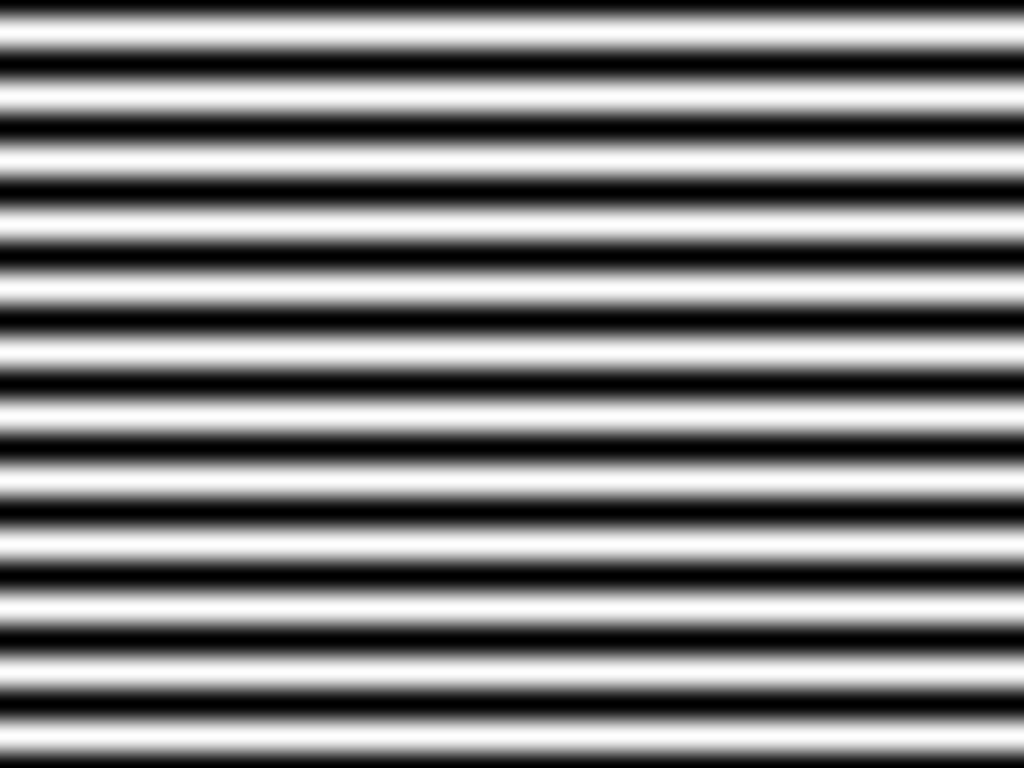
\includegraphics[width=5cm,height=5cm]{../img_source/phase_hor_1.jpg}}
\node at (0.0,-3) {\color{red} Projector image};
\pgftext[at=\pgfpoint{6cm}{0cm}]{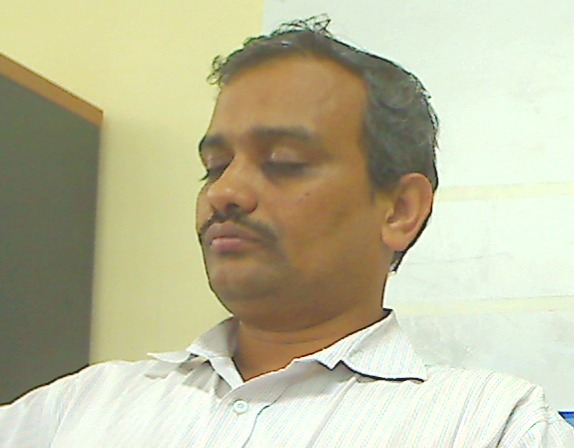
\includegraphics[width=5cm,height=5cm]{../img_source/face_2d.jpg}}
\node at (6,-3){\color{red} Camera image};
\pgftext[at=\pgfpoint{3cm}{9cm}]{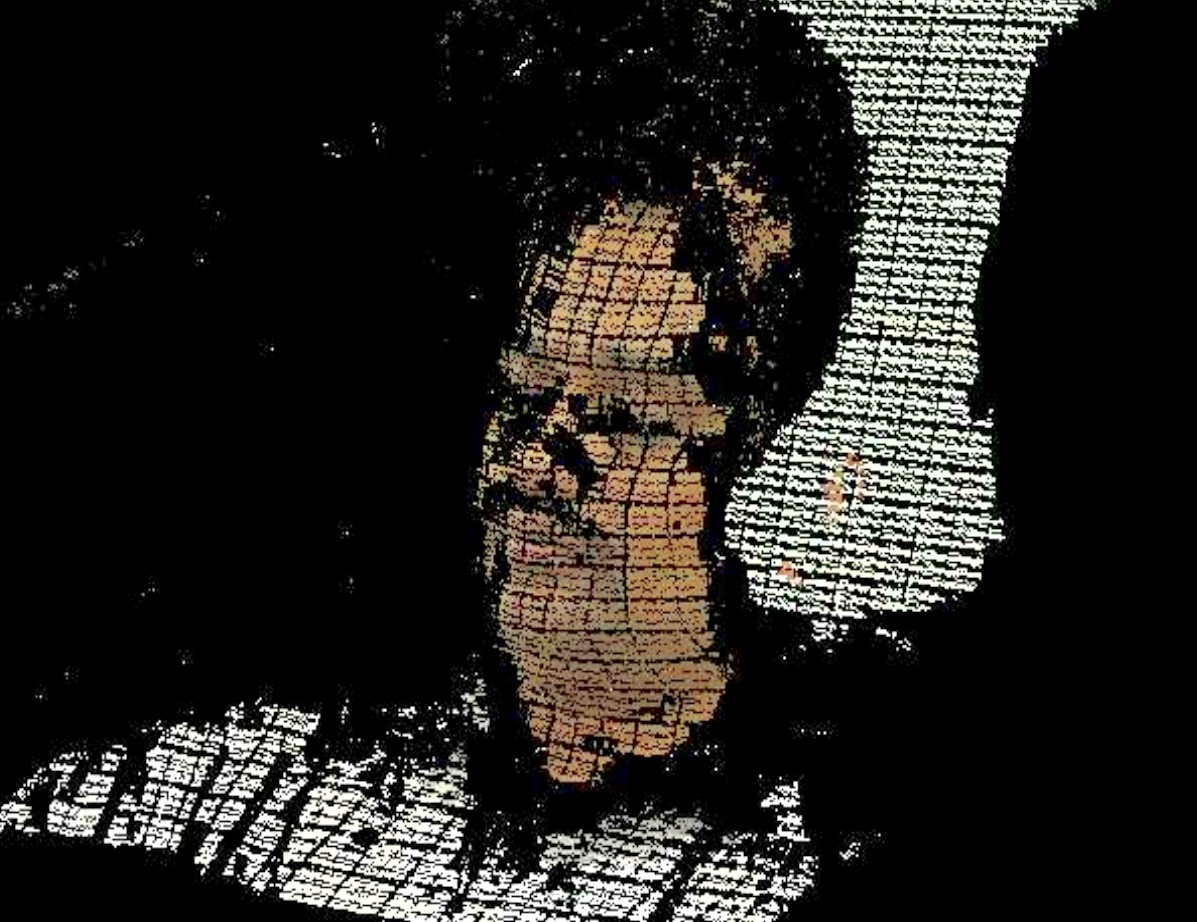
\includegraphics[width=5cm,height=5cm]{../img_source/face_3d.jpg}}
\node at (3,12){\color{red} Real-world object};
\draw [->](0,0)--(3.2,8);
\draw [->](3.2,8)--(6.1,-.7);
\draw[.] (6,0);
\fill [green] (3.2,8) circle[radius=2pt];
\fill [green] (6.1,-.7) circle[radius=2pt];
\fill [green] (0.0,0.0) circle[radius=2pt];
\end{tikzpicture}
\caption{Stereo correspondence and triangulation}
\label{fig:correspond_triangulate}
\end{figure}
\FloatBarrier
In figure~\ref{fig:correspond_triangulate}, a point in \textit{Projector image} is related to a point in \textit{Camera image} because they are 2D projections of a common point in the scene using the estimated stereo-correspondence. Once system is calibrated, ray-ray intersection between optical ray of camera and that of corresponding projector pixel gives the (X,Y,Z) coordinates of real-world point in \textit{physical unit} like `mm', `m' etc. \newline

\indent Figure~\ref{fig:arch} graphically represents the layout of our 3D scanner system, which can be referred during thesis. Working of \textbf{\textit{System calibration module}} is documented in chapter-2. \textbf{\textit{Pattern generation, Pattern projection and capture, Phase wrapper, Phase unwrapper, Absolute phase computation modules}} are explained in chapter-3. \textbf{\textit{Triangulation module}} has been described in chapter-4. 

\begin{figure}[!h]
\centering
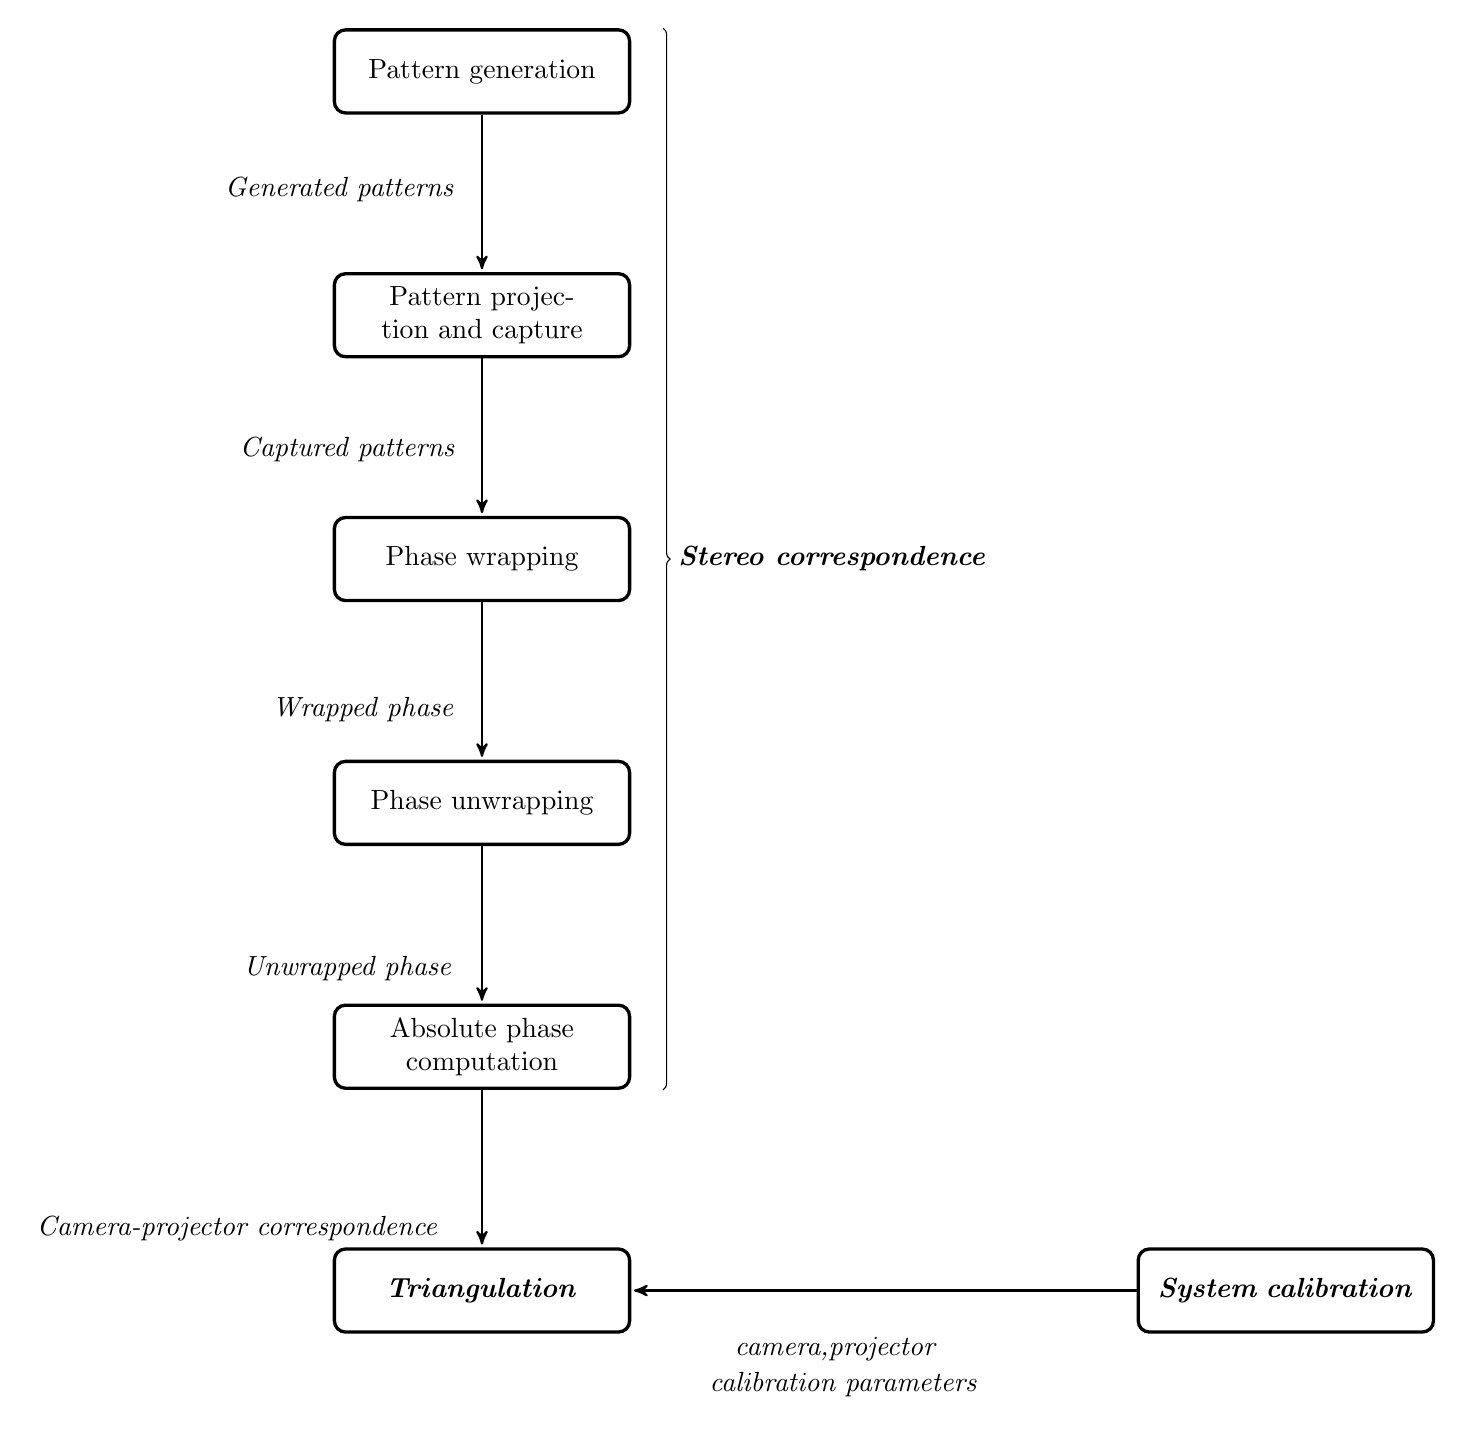
\begin{tikzpicture}
  [node distance=2.0cm,
  start chain=going below,]
     \node[punktchain, join] (intro) {Pattern generation};
     \node[punktchain, join] (probf)      {Pattern projection and capture};
     \node[punktchain, join] (investeringer)      {Phase wrapping};
     \node[punktchain, join] (perfekt) {Phase unwrapping};
     \node[punktchain,join] (emperi) {Absolute phase computation};
\node[punktchain,join](triangulate){\textbf{\textit{Triangulation}}};
\begin{scope}[start branch=x,every join/.style={->,thick,shorten <=1pt},]
\node[punktchain,on chain=going left,join=by {<-},node distance=-14.0cm](calib) {\textbf{\textit{System calibration}}};
\end{scope}

\draw[tuborg, decoration={brace}] let 
  \p1=(intro.north), \p2=(emperi.south) in 
   ($(2.3, \y1)$) -- ($(2.3,\y2)$) node[tubnode] {\textbf{\textit{Stereo correspondence}}};

\node at (-1.8,-1.5) {\textit{Generated patterns}};

\node at (-1.7,-4.8){\textit{Captured patterns}};

\node at (-1.5,-8.1){\textit{Wrapped phase}};

\node at (-1.7,-11.4){\textit{Unwrapped phase}};

\node at (-3.1,-14.7){\textit{Camera-projector correspondence}};

\node[above] at (4.5,-16.5){\textit{camera,projector}}; 
\node[below] at (4.6,-16.4){\textit{calibration parameters}};
\end{tikzpicture}
\caption{Architecture of the developed system}
\label{fig:arch}
\end{figure}



\chapter{System calibration} 
 
         
For performing non-metric reconstruction only point-to-point correspondences between camera and projector are needed to perform triangulation[3]. But to relate the depth computed using triangulation with physical metrics such as 'mm', 'cm' etc there is need to relate the camera and projector geometry with physical measurement units, this task is accomplished by process of System calibration.  Calibration is a process of determining intrinsic and extrinsic characteristics of the imaging devices(camera and projector in our case). Intrinsic characteristics include focal length, coordinates of principal points of lens used in camera and projectors, image axis skew coefficients and lens distortion coefficients. Extrinsic characteristics include rigid-body transformations that can transform a point represented in World-coordinate system to individual coordinates systems of camera and projector. \newline 

 
Above discussion clearly implies the need to establish defining equations which relate a real-world three dimensional point(with coordinates expressed in \textit{physical} units) with pixel coordinates in camera(or projector). For this purpose a projective model of camera which applies to projector as well is introduced in the next section which clearly describes the problem of calibration, following which the current approaches and the approach used in this work to solve this problem will be reviewed. In the end, a note on \textit{relative extrinsic calibration} of projector-camera system is mentioned, which is a process of determining relative rotation and translation of camera and projector coordinate systems which in simple words means to determine the relative orientation and position of camera with respect to projector or vice-versa.   
  
\section{Camera model}   
Camera model is a concise mathematical abstraction of the internal(i.e., its optics and sensor arrangement) and external(i.e., its position relative to a scene) geometry of camera which is responsible for the imaging process. In this section, these geometric parameters will be described and hence the imaging process. Camera model described here is referred from seminal paper by [8]. Other calibration techniques also follow variants of this formulation. Relatively recent work in [9] has shown projector to be \textit{inverse-camera} hence further discussion on camera calibration holds equally to projector as well. Section 2.4.2 will describe how  projector was calibrated similar to camera with a real example. In next subsection the coordinate-systems which are relevant for geometric modeling of imaging process under consideration will be described.  
  
\subsection{Graphical abstraction}  
In this subsection the graphical model of camera depicting coordinate systems involved in transforming a real world 3D point to camera 2D coordinate representation will be described.
   
\paragraph{World-coordinate system.}  
World-coordinate system defines the reference frame in the real world that will be used for defining the positions of object in scene in physical units. Typically any location in the real scene can be used as origin for world coordinate system axes. For example in this work world coordinate system origin was assumed to be present at a corner on a wall.  
  
\paragraph{Camera-coordinate system.}  
This is a 3D reference coordinate-system internal to camera, it is similar to world coordinate system since it also works in physical units. Its origin is assumed to be at center of projection of camera. It is used to generate 3D interpretation of the scene from camera viewpoint.  
  
\paragraph{Image-coordinate system.}  
This is a 2D reference coordinate-system for indexing points in the real-image. Note here \textit{real} means that it can take real values as coordinates. It is used to index the points in perspective projection of 3D world.  
  
\paragraph{Computer-frame coordinate system.}  
This is a 2D reference coordinate-system which indexes pixels in the computer-frame. It can only have integral coordinates. Images with which we normally interact are indexed with respect to this coordinate system. \newline  
  
Figure~\ref{fig:coordinate_systems}\footnote{Figure source: Refer~\cite{8}} illustrates the coordinate systems except computer-frame coordinate system since it is not geometrically connected with other coordinate systems:  
  
%\begin{figure}[hb]  
%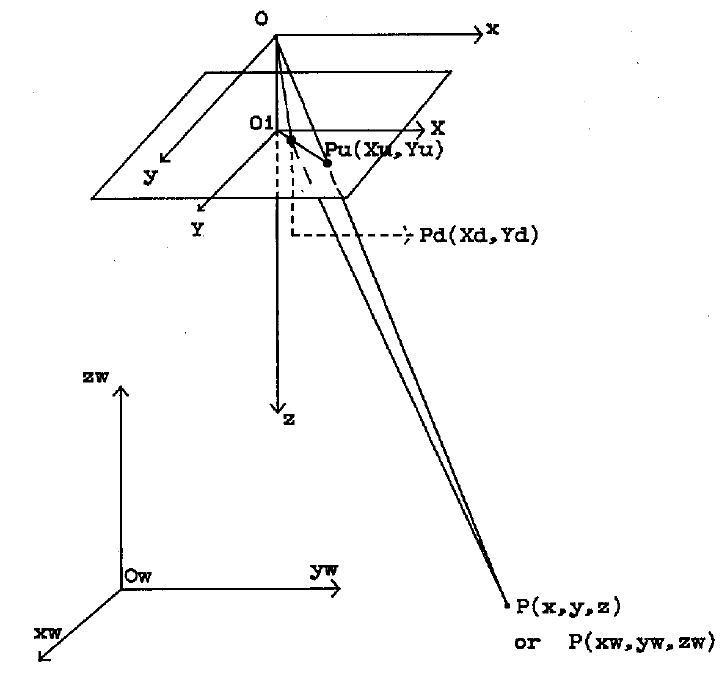
\includegraphics[width=10cm,height=10cm]{../img_source/coordinate_systems.jpg}  
%\caption{Transformation of a real world 3D point from world coordinate system to computer-buffer coordinate system}  
%\label{fig:coordinate_systems}
%\end{figure}  

\begin{figure}[ht]
\centering
\begin{tikzpicture}
% world coordinate system
\draw[->] (0,0)--(0,3);%Y
\draw[->] (0,0)--(3,0);%X
\draw[->] (0,0)--(-1.5,-1.5);%Z
\node[below] at (0,0) {\textbf{$O_w$}};
\node[below] at (3,0) {\textbf{$X_w$}};
\node[left] at (0,3) {\textbf{$Y_w$}};
\node[below] at (-1.0,-1.5) {\textbf{$Z_w$}};

% camera coordinate system
\draw[->] (2,9)--(2,4);%Z
\draw[->] (2,9)--(5,9);%X
\draw[->] (2,9)--(1,6);%Y
\node[left] at (2,9) {\textbf{$O_c$}};
\node[above] at (5,9) {\textbf{$X_c$}};
\node[below] at (2,4) {\textbf{$Z_c$}};
\node[below] at (1,6) {\textbf{$Y_c$}};

% camera-image coordinate system
\draw (0.5,8)--(6,8);
\draw (0.5,8)--(-0.5,6);
\draw (6,8)--(5,6);
\draw (-0.5,6)--(5,6);

\node[left] at (2,7.5) {\textbf{$O_i$}};
\fill [black] (2,7.5) circle[radius=2pt];

\draw[->] (2,7.5)--(4,7.5);
\draw[->] (2,7.5)--(1,4.5);
\node[below] at (4,7.5){\textbf{$X_i$}};
\node[left] at (1,4.5){\textbf{$Y_i$}};

%3d point
\node[below] at (7,-1){\textbf{$P$}};
\fill [black] (7,-1) circle[radius=2pt];

\draw (7,-1)--(2.9,7.3);
\fill[black] (2.9,7.3) circle[radius=2pt];
\node[below] at (2.9,7.3) {\textbf{$P_u$}};

\draw (2.9,7.3)--(2,9);


\node[below] at (2.5,6.9) {\textbf{$P_d$}};
\fill[black] (2.5,6.9) circle[radius=2pt];

\draw (7,-1)--(2.5,6.9);
\draw (2.5,6.9)--(2,9);

\end{tikzpicture}
\caption{Transformation of a real world 3D point from world coordinate system to computer-buffer coordinate system}  
\label{fig:coordinate_systems}
\end{figure}  


Here points $O_w,O_c$ and $O_i$ represent origins of world,camera and real-image coordinate systems respectively. Further, axes $X_w,Y_w$ and $Z_w$ represent the world-coordinate system, axes $X_c,Y_c$ and $Z_c$ denote the camera coordinate system, similarly axes $X_i$ and $Y_i$ show the 2D real-image coordinate system, $P$ is a real-world point, $P_u$ is the ideal projection of $P$ on real-image plane(i.e., image-coordinate system), $P_d$ is corresponding distorted projection which differ from $P_u$ due to practical imperfections in camera system. Equations relating these coordinate systems are described in the following paragraphs of this section.  
  
\subsection{Mathematical abstraction}  
In this subsection, the actual mathematical form of camera imaging process which is used for transforming a real-world 3D point to a computer-buffer pixel will be sequentially described. This involves a series of coordinate transformations which are described here.   

\paragraph{1.Rigid body transformations from object world-coordinate system to camera coordinate system.}  
Points in the world-coordinate coordinates system (x\textsubscript{w},y\textsubscript{w},z\textsubscript{w}) are transformed to the camera-coordinate system (x\textsubscript{c},y\textsubscript{c},z\textsubscript{c}). To model this process, rotation(R) and translation(T) matrices are used as:  
  
\begin{equation}  
\begin{bmatrix}  
x_c \\  
y_c \\  
z_c  
\end{bmatrix}  
=  
R*   \begin{bmatrix}  
      x_w \\  
      y_w \\  
      z_w  
      \end{bmatrix}  
+T  
\end{equation}  
where $R=\begin{bmatrix}  
         r_{1,1} & r_{1,2} & r_{1,3} \\  
         r_{2,1} & r_{2,2} & r_{2,3} \\  
         r_{3,1} & r_{3,2} & r_{3,3}   
         \end{bmatrix}$  
,$T=\begin{bmatrix}  
    t_x \\  
    t_y \\  
    t_z  
   \end{bmatrix}$ \newline  
  
  
Rotation and translation parameters are called \textit{extrinsic parameters} of camera/projector. It should be noted here that rotation followed by translation is used since it ensures unique transformations, whereas translation followed by rotation can result in multiple possible transformations[8].  
  
  
  
\paragraph{2.Perspective transformation from camera-coordinates to real-image coordinates.}  
In this step, 3D scene as viewed from camera-coordinate origin is perspective projected to a plane. Hence it is a 3D to 2D transformation resulting in loss of Z-coordinate(i.e., depth) since multiple points are projected onto same point in the image-plane. Following equations describe this process:  
  
\begin{equation}  
\begin{bmatrix}  
x_u \\  
y_u  
\end{bmatrix}  
=\bigg(\frac{f}{z_c}\bigg)*  
\begin{bmatrix}  
x_c \\  
y_c  
\end{bmatrix}  
\end{equation}  
  
\noindent  
where \textit{f} represents the focal length of camera/projector lens. (x\textsubscript{u},y\textsubscript{u}) is the perspective projection of point (x\textsubscript{c},y\textsubscript{c},z\textsubscript{c}) on real-image plane.  
  
\paragraph{3.Radial and tangential lens distortion.}  
In this step, real-image coordinates are distorted due to radially imperfections in practical lens which is characterized by \textit{radial distortion} and oblique alignment of principal plane of lens and sensor-plane which is characterized by \textit{tangential distortion}. Although Tsai's work only accounted for radial distortions subsequent works have accounted for tangential[10] and prism distortions[11] also in an attempt to increase the accuracy of estimated calibration parameters further. Following equations describes the effect of radial and tangential distortion on \textit{ideal} image coordinates:  
\begin{equation}  
\begin{aligned}
& x_d=x_u(1+k_1r^2+k_2r^4+k_3r^6+...)+2p_1x_uy_u+p_2(r^2+2x_u) \\
& y_d=y_u(1+k_1r^2+k_2r^4+k_3r^6+...)+2p_2x_uy_u+p_1(r^2+2y_u)
\end{aligned}
\end{equation}  
\noindent  
where,\newline
$(x_d,y_d)$: distorted image coordinates\newline
$(k_1,k_2,k_3)$: radial distortion coefficients\newline
$(p_1,p_2)$: tangential distortion coefficients\newline
$r=\sqrt[2]{X_u^2+Y_u^2}$
  
\paragraph{4.Transforming real-image coordinates to computer-frame coordinates.}  
Finally to map 3D world-coordinates to frame coordinates of camera, i.e., the pixels that we see, following equations are assumed:  
\begin{equation}  
\begin{bmatrix}  
x_f \\  
y_f  
\end{bmatrix}  
=\begin{bmatrix}  
s_x*(d_x^{'})^{-1}*x_d\\  
d_y^{-1}*y_d  
\end{bmatrix}   
+\begin{bmatrix}  
C_x \\  
C_y  
\end{bmatrix}  
\end{equation}  
\noindent  
where,\newline  
$(x_f,y_f)$:computer frame-buffer coordinates for point $(x_d,y_d)$ \newline  
$s_x$:uncertainty image-scale factor \newline  
$d_x$:center-to-center distance between sensor cells along X-direction\newline  
$N_{cx}$:Number of sensors along X-direction\newline  
$N_{fx}$:Number of pixels along X-line sampled by computer\newline  
$d_x^{'}=d_x*\left(\frac{N_{cx}}{N_{fx}}\right)$\newline\newline  
It should be noted that at full camera resolution there is one-to-one relation between number of sensor elements and number of pixels in computer-frame buffer hence $N_{cx}=N_{fx}$ and hence $d_x^{'}=d_x$ but in general $d_x^{'}>=d_x$. [8] attributed $s_x$ to be due to  possibility of mismatch between camera image acquisition hardware and camera scanning hardware. Figure~\ref{fig:cam_model_pipeline}\footnote{Figure source: Refer~\cite{8}} illustrates the complete imaging process. 
%\begin{figure}[ht]  
%\centering  
%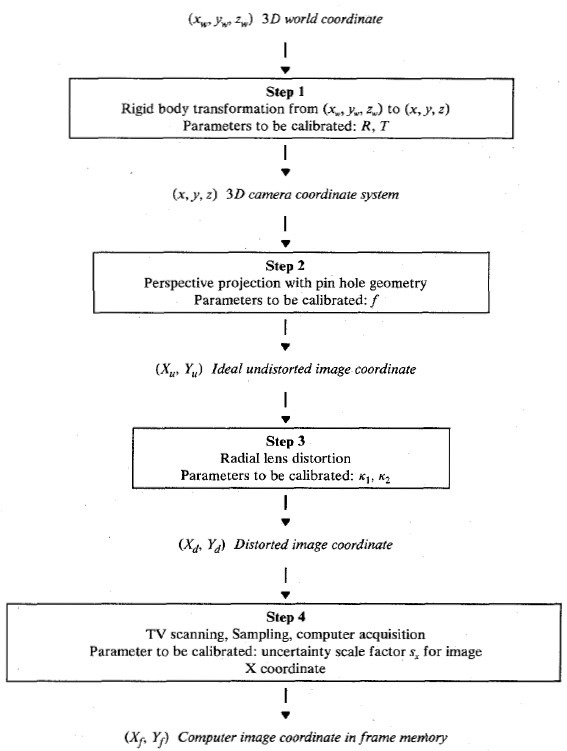
\includegraphics[width=10cm,height=14cm]{../img_source/cam_model_pipeline.jpg}  
%\caption{Camera model pipeline}  
%\label{fig:cam_model_pipeline}
%\end{figure}  
\begin{figure}
\centering
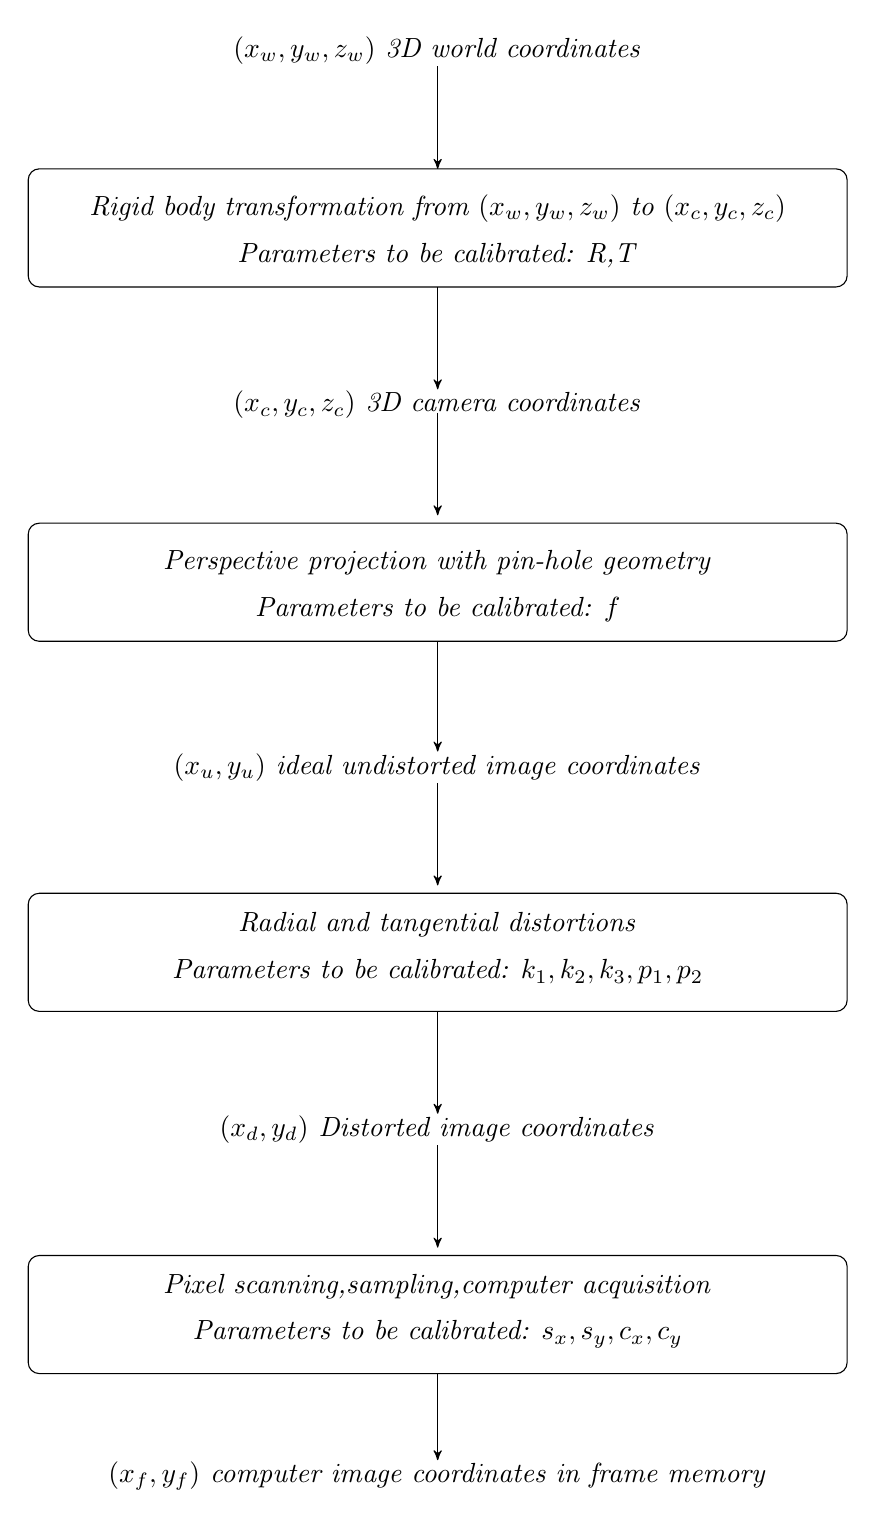
\begin{tikzpicture}
\node at (0,0) {\textit{$(x_w,y_w,z_w)$ 3D world coordinates}};
\draw[->] (0,-0.2)--(0,-1.5);
\draw[rounded corners] (-5.2,-1.5) rectangle (5.2,-3);
\node at (0,-2.0){\textit{Rigid body transformation from $(x_w,y_w,z_w)$ to $(x_c,y_c,z_c)$}};
\node at (0,-2.6) {\textit{Parameters to be calibrated: R,T}};

\draw[->] (0,-3)--(0,-4.3);
\node at (0,-4.5) {\textit{$(x_c,y_c,z_c)$ 3D camera coordinates}};
\draw[->] (0,-4.6)--(0,-5.9);
\draw[rounded corners] (-5.2,-6.0) rectangle (5.2,-7.5);
\node at (0,-6.5) {\textit{Perspective projection with pin-hole geometry}}; \node at (0,-7.1) {\textit{Parameters to be calibrated: $f$}};

\draw[->] (0,-7.5)--(0,-8.9);
\node at (0,-9.1) {\textit{$(x_u,y_u)$ ideal undistorted image coordinates}};

\draw[->] (0,-9.3)--(0,-10.6);
\draw[rounded corners] (-5.2,-10.7) rectangle (5.2,-12.2);
\node at (0,-11.1) {\textit{Radial and tangential distortions}};
\node at (0,-11.7) {\textit{Parameters to be calibrated: $k_1,k_2,k_3,p_1,p_2$}};

\draw[->] (0,-12.2)--(0,-13.5);
\node at (0,-13.7) {\textit{$(x_d,y_d)$ Distorted image coordinates}};
\draw[->] (0,-13.9)--(0,-15.2);
\draw[rounded corners] (-5.2,-15.3) rectangle (5.2,-16.8);

\node at (0,-15.7) {\textit{Pixel scanning,sampling,computer acquisition}}; 
\node at (0,-16.3) {\textit{Parameters to be calibrated: $s_x,s_y,c_x,c_y$}};

\draw[->] (0,-16.8)--(0,-17.9);
\node at (0,-18.1) {\textit{$(x_f,y_f)$ computer image coordinates in frame memory}};
\end{tikzpicture}
\caption{Camera model pipeline}  
\label{fig:cam_model_pipeline}
\end{figure}

\noindent  
So based on above discussion we can deduce that to define the geometric imaging process of camera(or projector) we have to estimate following parameters:
\begin{enumerate}  
\item Internal parameters:
\begin{enumerate}
\item Camera lens focal length
\item Position of principal point on the real-image plane
\item Lens distortion parameters
\end{enumerate}
\item External parameters:
\begin{enumerate}
\item Rotation between camera-coordinate system and world-coordinate system  
\item Translation between camera-coordinate system and world-coordinate system  
\end{enumerate}
\end{enumerate}  
  
  
  
\section{Current approaches:A review}  
A taxonomy was proposed by [10] for camera calibration approaches based on their requirement of additional calibration objects as:  
\paragraph{a) Photogrammetric calibration.}  
These techniques perform camera calibration by observing a calibration object. Calibration object can be any object with known geometry i.e., we know world-coordinates of feature-points on the object that we want to use for calibration. In this category many techniques for both 3D and 2D calibration objects were proposed. For example use of 3D calibration object with three orthogonal planes or planar calibration rigs with known translation across its views have been used for calibration[8] although requiring elaborate setup for calibration and often time-consuming.  
\paragraph{b) Self-calibration.}  
These techniques are more flexible than photogrammetric techniques in that they do not require an explicit calibration rig for calibration, but by moving the camera across a static rigid scene they determine constraints on internal parameters of camera that can be used for calibration[12][13]. Other than these techniques there are techniques that do not fall into these categories
such as camera calibration using vanishing points for orthogonal directions[14], calibration from pure rotation[15]. In this work, a photogrammetric method for camera and projector calibration was used. Following paragraphs will briefly describe the details of some highly cited and practically used algorithms in chronological order.\newline  
  
\paragraph{R.Y.Tsai's algorithm.}  
Tsai's algorithm restricts the lens-distortion effects to only radial distortion and do not account for skewness or lack of orthogonality of projection. Calibration was divided in 2 separate stages. In first stage all extrinsic parameters except for $t_z$ are computed using the \textit{Radial alignment constraint(RAC)} shown in figure~\ref{fig:rac}\footnote{Figure source: Refer~\cite{16}}. If assumed lens distortion is only \textit{radial}, then the direction of vector $O_iP_d$ remains unchanged and is parallel to vector $P_{oz}P_w$. Tsai showed that RAC is independent of magnitude of effective focal length, radial distortion coefficients and position of point $P_w$ along z-axis. He further proved that this constraint is sufficient to estimate 3D rotation and translation of $P_w$ along X and Y axes. \newline   
\begin{figure}[ht]  
\centering  
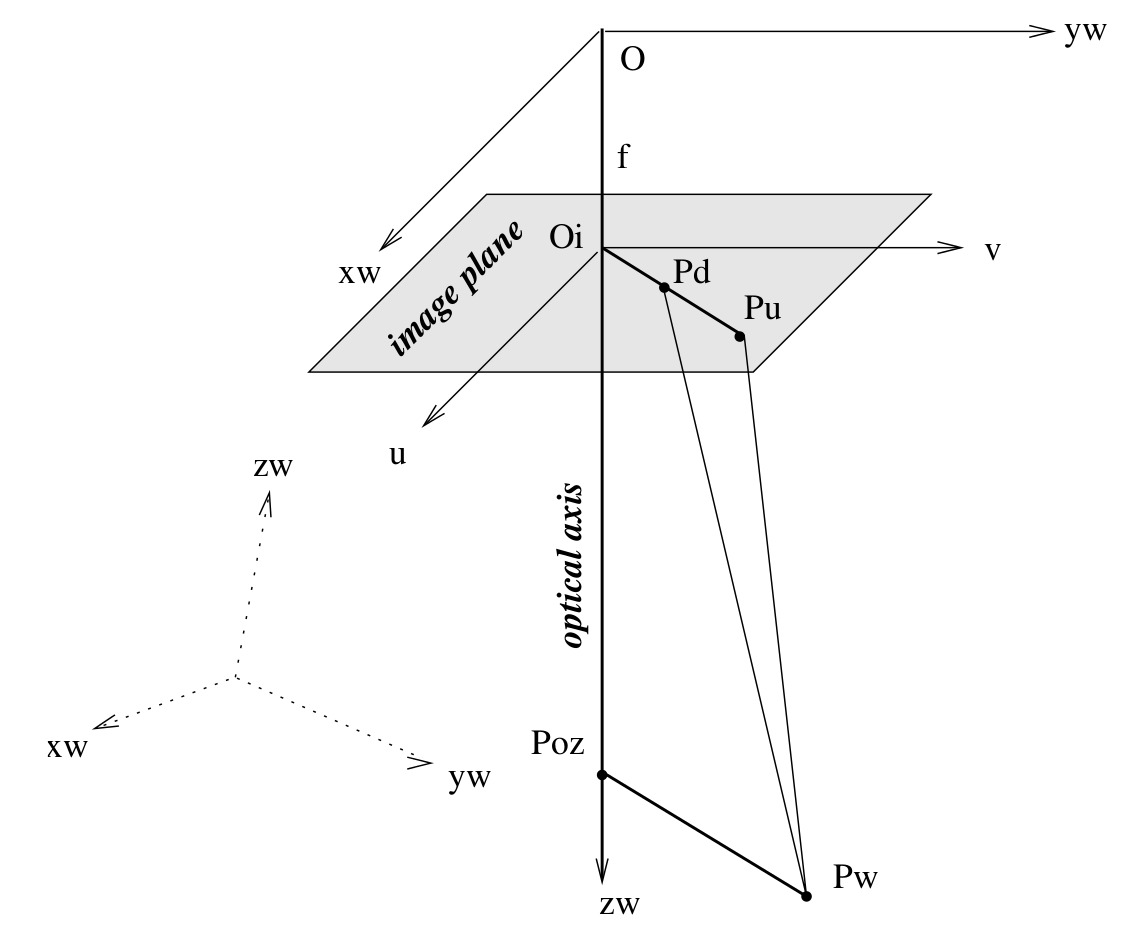
\includegraphics[width=13cm,height=10cm]{../img_source/tsai_rac.jpg}  
\caption{Radial alignment constraint used in Tsai's algorithm}  
\label{fig:rac}
\end{figure}  
  
\noindent  
In second stage effective focal length, distortion coefficients and $t_z$ are estimated using non-linear optimization.  
  
  
\paragraph{Z.Zhang's algorithm.}  
Z.Zhang proposed a plane based camera calibration algorithm[10]. It first acquires real-world coordinate to camera image coordinate correspondences using planar calibration board. Then it estimates all intrinsic and extrinsic parameters using a closed-form solution. This closed form solution assumes zero lens distortion and is based on two constraints on intrinsic parameters derived from the \textit{orthonormality} of rotation vector expressed in equations 2.5,2.6.  
\begin{equation}  
h_1^TA^{-T}A^{-1}h_2=0  
\end{equation}  
\begin{equation}  
h_1^TA^{-T}A^{-1}h_1=h_2^{T}A^{-T}A^{-1}h_2  
\end{equation}  
\noindent  
where,\newline  
$h_i$: $i^{th}$ column vector of Homography\newline  
$A$: Camera projective matrix\newline  
  

Further, the coefficients of radial distortion $k_1,k_2$ are estimated by solving linear least squares expressed in equation 2.7.  
\begin{equation}  
\begin{bmatrix}  
(u-u_0)(x^2+y^2) & (u-u_0)(x^2+y^2)^2 \\  
(v-v_0)(x^2+y^2) & (v-v_0)(x^2+y^2)^2  
\end{bmatrix}  
\begin{bmatrix}  
k_1 \\  
k_2  
\end{bmatrix}  
=\begin{bmatrix}  
u'-u \\  
v'-v  
\end{bmatrix}  
\end{equation}\newline  
\noindent  
where,\newline  
$(u,v)$: ideal pixel image coordinates\newline  
$(u_0,v_0)$: coordinates of principal point\newline  
$(x,y)$: ideal normalized image coordinates\newline  
  

\noindent  
Estimated values of all parameters are considered as initial input for non-linear least squares minimization which minimizes expression in equation 2.8.  
\begin{equation}  
\sum_{i=1}^{m}\sum_{j=1}^{n}||m_{ij}-m'(A,k_1,k_2,R_i,t_i,M_j)||^2  
\end{equation}\newline  
\noindent  
where,\newline  
$m$: Total number of features on the calibration board \newline  
$n$: Total number views of planar calibration board \newline  
$M_j$: 3D coordinates of $j^{th}$ feature point on calibration board\newline  
$m_{ij}$: True 2D coordinates of projection of $M_j$ in camera image\newline   
$m'$: Estimated 2D coordinates for $M_j$ using calibration parameters\newline  
$R_i$: Rotation parameters for $i^{th}$ view used for calibration\newline  
$t_i$: Translation parameters for $i^{th}$ view used for calibration\newline  
  
\paragraph{J.Heikkila et al.'s algorithm.}  
This algorithm assumes a more elaborate camera model which includes both radial and tangential components as lens distortion coefficients. It first linearizes the camera model by ignoring lens distortion coefficients and performs linear parameter estimation using Direct Linear Transformation(DLT)[17]. Equation 2-9 shows the linear model solved using DLT method.\newline  
\begin{equation}  
La=0  
\end{equation}\newline  
\noindent  
where,\newline   
a=$\begin{bmatrix}  
a_{1,1} & a_{1,2} & a_{1,3} & a_{1,4} & a_{2,1} & a_{2,2} & a_{2,3} & a_{2,4} & a_{3,1} & a_{3,2} & a_{3,3} & a_{3,4}   
\end{bmatrix}$\newline  
\newline  
L=$\begin{bmatrix}  
X_1 & Y_1 & Z_1 & 1 & 0 & 0 & 0 & 0 & -X_1u_1 & -Y_1u_1 & -Z_1u_1 & -u_1 \\  
0 & 0 & 0 & 0 & X_1 & Y_1 & Z_1 & 1 & -X_1v_1 & -Y_1v_1 & -Z_1v_1 & -v_1 \\    
: & : & : & : &  :  &  :  &  :  & : &   :     &    :    &    :    &   : \\  
X_i & Y_i & Z_i & 1 & 0 & 0 & 0 & 0 & -X_iu_i & -Y_iu_i & -Z_iu_i & -u_i \\  
0 & 0 & 0 & 0 & X_i & Y_i & Z_i & 1 & -X_iv_i & -Y_iv_i & -Z_iv_i & -v_i \\  
: & : & : & : &  :  &  :  &  :  & : &   :     &    :    &    :    &   : \\  
X_n & Y_n & Z_n & 1 & 0 & 0 & 0 & 0 & -X_nu_n & -Y_nu_n & -Z_nu_n & -u_n \\  
0 & 0 & 0 & 0 & X_n & Y_n & Z_n & 1 & -X_nv_n & -Y_nv_n & -Z_nv_n & -v_n   
\end{bmatrix}$ \newline  
\newline  
\newline  
\noindent  
Here, $(X_i,Y_i,Z_i)$ denotes 3D coordinates of $i^{th}$ feature point used in calibration, $(u_i,v_i)$ denotes the corresponding 2D image coordinates, \textit{a} denotes the projective matrix mapping $(X_i,Y_i,Z_i)$ to $(u_i,v_i)$.  
In second step, Gaussian noise model is assumed and a non-linear least square minimization is performed to minimize equation 2-10.\newline    
\begin{equation}  
F=\sum_{i=1}^N\big[(U_i-u_i)^2+(V_i-v_i)^2\big]  
\end{equation}  
\noindent  
where, \textit{N} is the number of observations, $(U_i,V_i)$ are the observed 2D coordinates of $i^{th}$ feature point, $(u_i,v_i)$ are corresponding 2D coordinates estimated using calibration parameters.  
  
  
  
\section{Approach followed in this work}  
For camera and projector calibration an extension of [10] method was used which was first described and developed in [18] and later ported to OpenCV. Unfortunately, author in [18] has not published the details of algorithm except describing the approach to be based on camera model described in [17] and implementation as a variant of [10] hence  
OpenCV documentation other than reading the source code itself is the only source of  
theoretical information on this technique. During this project work, an effort is initiated  
to fully understand the calibration algorithms and effect of each calibration  
parameters on accuracy of 3D reconstruction by actually implementing an algorithm  
so that every input to the algorithm can be changed and its effect seen. For which technique described in [17] was selected and partially implemented. Here a brief outline of camera/projector calibration algorithm implemented in OpenCV/Matlab[18][19] is presented:  
\begin{enumerate}
\item A planar calibration board is selected with known world-coordinates of reference points on it.  
\item Calibration board is shown for multiple views(at least 2) in front of camera by varying its rotation and translation(amount need not be known) with respect to camera and for every pose feature-points are  
detected in camera.  
\item After all such views are captured and feature-points detected, homography for each view is calculated.  
\item Closed form solution of intrinsic parameters from homographies using orthogonality of vanishing points is computed but unlike [10] no initial estimates of distortion coefficients are computed.  
\item Initial estimates of calibration parameters computed earlier are given as input to Maximum likelihood estimator Levenberg-Marquardt algorithm[20] to refine the parameters.Output of this process is a set of calibration parameters which optimally satisfy the maximum likelihood criteria.  
\end{enumerate}

 
\paragraph{Algorithm for extrinsic calibration of camera and projector.}  
Extrinsic parameters relate camera-coordinate system and projector-coordinate system to world-coordinate system. For  
extrinsic calibration, OpenCV[21] performs minimization of re-projection error between  
observed point projections given as input(i.e., image points) and projection computed  
by applying the estimated model to the given object points. Extrinsic parameters that  
minimize this criteria are considered as the optimal pose(Rotation and translation)  
parameters.  
  
\paragraph{A note on Relative calibration of projector and camera.}  
After camera and projector are calibrated extrinsically, there is need to relate their  
coordinate-systems with each other so that a point in projector coordinate-system can  
also be expressed in terms of camera-coordinate system. This is required because of  
an implicit assumption in triangulation is that it requires intersection of optical rays from  
camera and projector, which is possible only if we can express both rays in a common  
coordinate-system either in that of camera or projector. This is achieved  
using our world-coordinate system as a common link between projector and camera.  
Following equations relate camera-coordinate system to projector-coordinate system  
via world-coordinate system[22]:  
\begin{equation}  
\begin{bmatrix}  
P_c \\  
P_p  
\end{bmatrix}  
=\begin{bmatrix}  
R_{wc}*P_w \\  
R_{wp}*P_w  
\end{bmatrix}  
+\begin{bmatrix}  
T_{wc} \\  
T_{wp}  
\end{bmatrix}  
\end{equation}  
hence,\newline  
$P_c=\underbrace{(R_c*R_p^{-1})}_{R_{pc}}*P_p+\underbrace{(T_c-R_c*R_p^{-1}*P_p)}_{T_{pc}}$  
  
\noindent  
where,\newline  
$P_w$:A point in world coordinate system\newline  
$P_c$:Representation of $P_w$ with respect to camera coordinate system\newline  
$P_p$:Representation of $P_w$ with respect to projector coordinate system\newline  
$R_{wc}$:Rotation transformation from world-to-camera coordinate system\newline  
$R_{wp}$:Rotation transformation from world-to-projector coordinate system\newline  
$T_{wc}$:Translation transformation from world-to-camera coordinate system\newline  
$T_{wp}$:Translation transformation from world-to-projector coordinate system\newline  
$R_{pc}$:Rotation transformation from projector-to-camera coordinate system\newline  
$T_{pc}$:Translation transformation from projector-to-camera coordinate system\newline  
  
Here $R_{pc}$ and $T_{pc}$ are the final outcomes which allows us to map a point in projector coordinate system to camera coordinate system which is an requirement for performing stereo-triangulation.  
  
\section{Working of developed system calibration module}  
System calibration is composed of camera calibration, projector calibration and relative extrinsic calibration of camera with respect to projector. A module for system calibration was developed which performs above mentioned functions using OpenCV camera calibration and extrinsic calibration algorithms. This section first describes the system setup and then explains the practical procedure for camera, projector and extrinsic calibration of projector with respect to camera.  
  
\paragraph{System setup.}  
In this work,Logitech Quickcam sphere AF web-cam at 1600X1200 pixels  
resolution was as a capture device, Sharp PG-F200X projector at 1024X768 pixels resolution was used for pattern projection, and 4 markers(shown in figure~\ref{fig:calib_setup} as `black' points) as world coordinate references forming a  
rectangular region of 1900mm X 1700mm and a physical checkerboard with square  
size 25.6mm arranged in a 10X8 square grid. Figure~\ref{fig:calib_setup} shows setup of our 3D  
scanner system:\newline  
  
\begin{figure}[htbp]  
\centering  
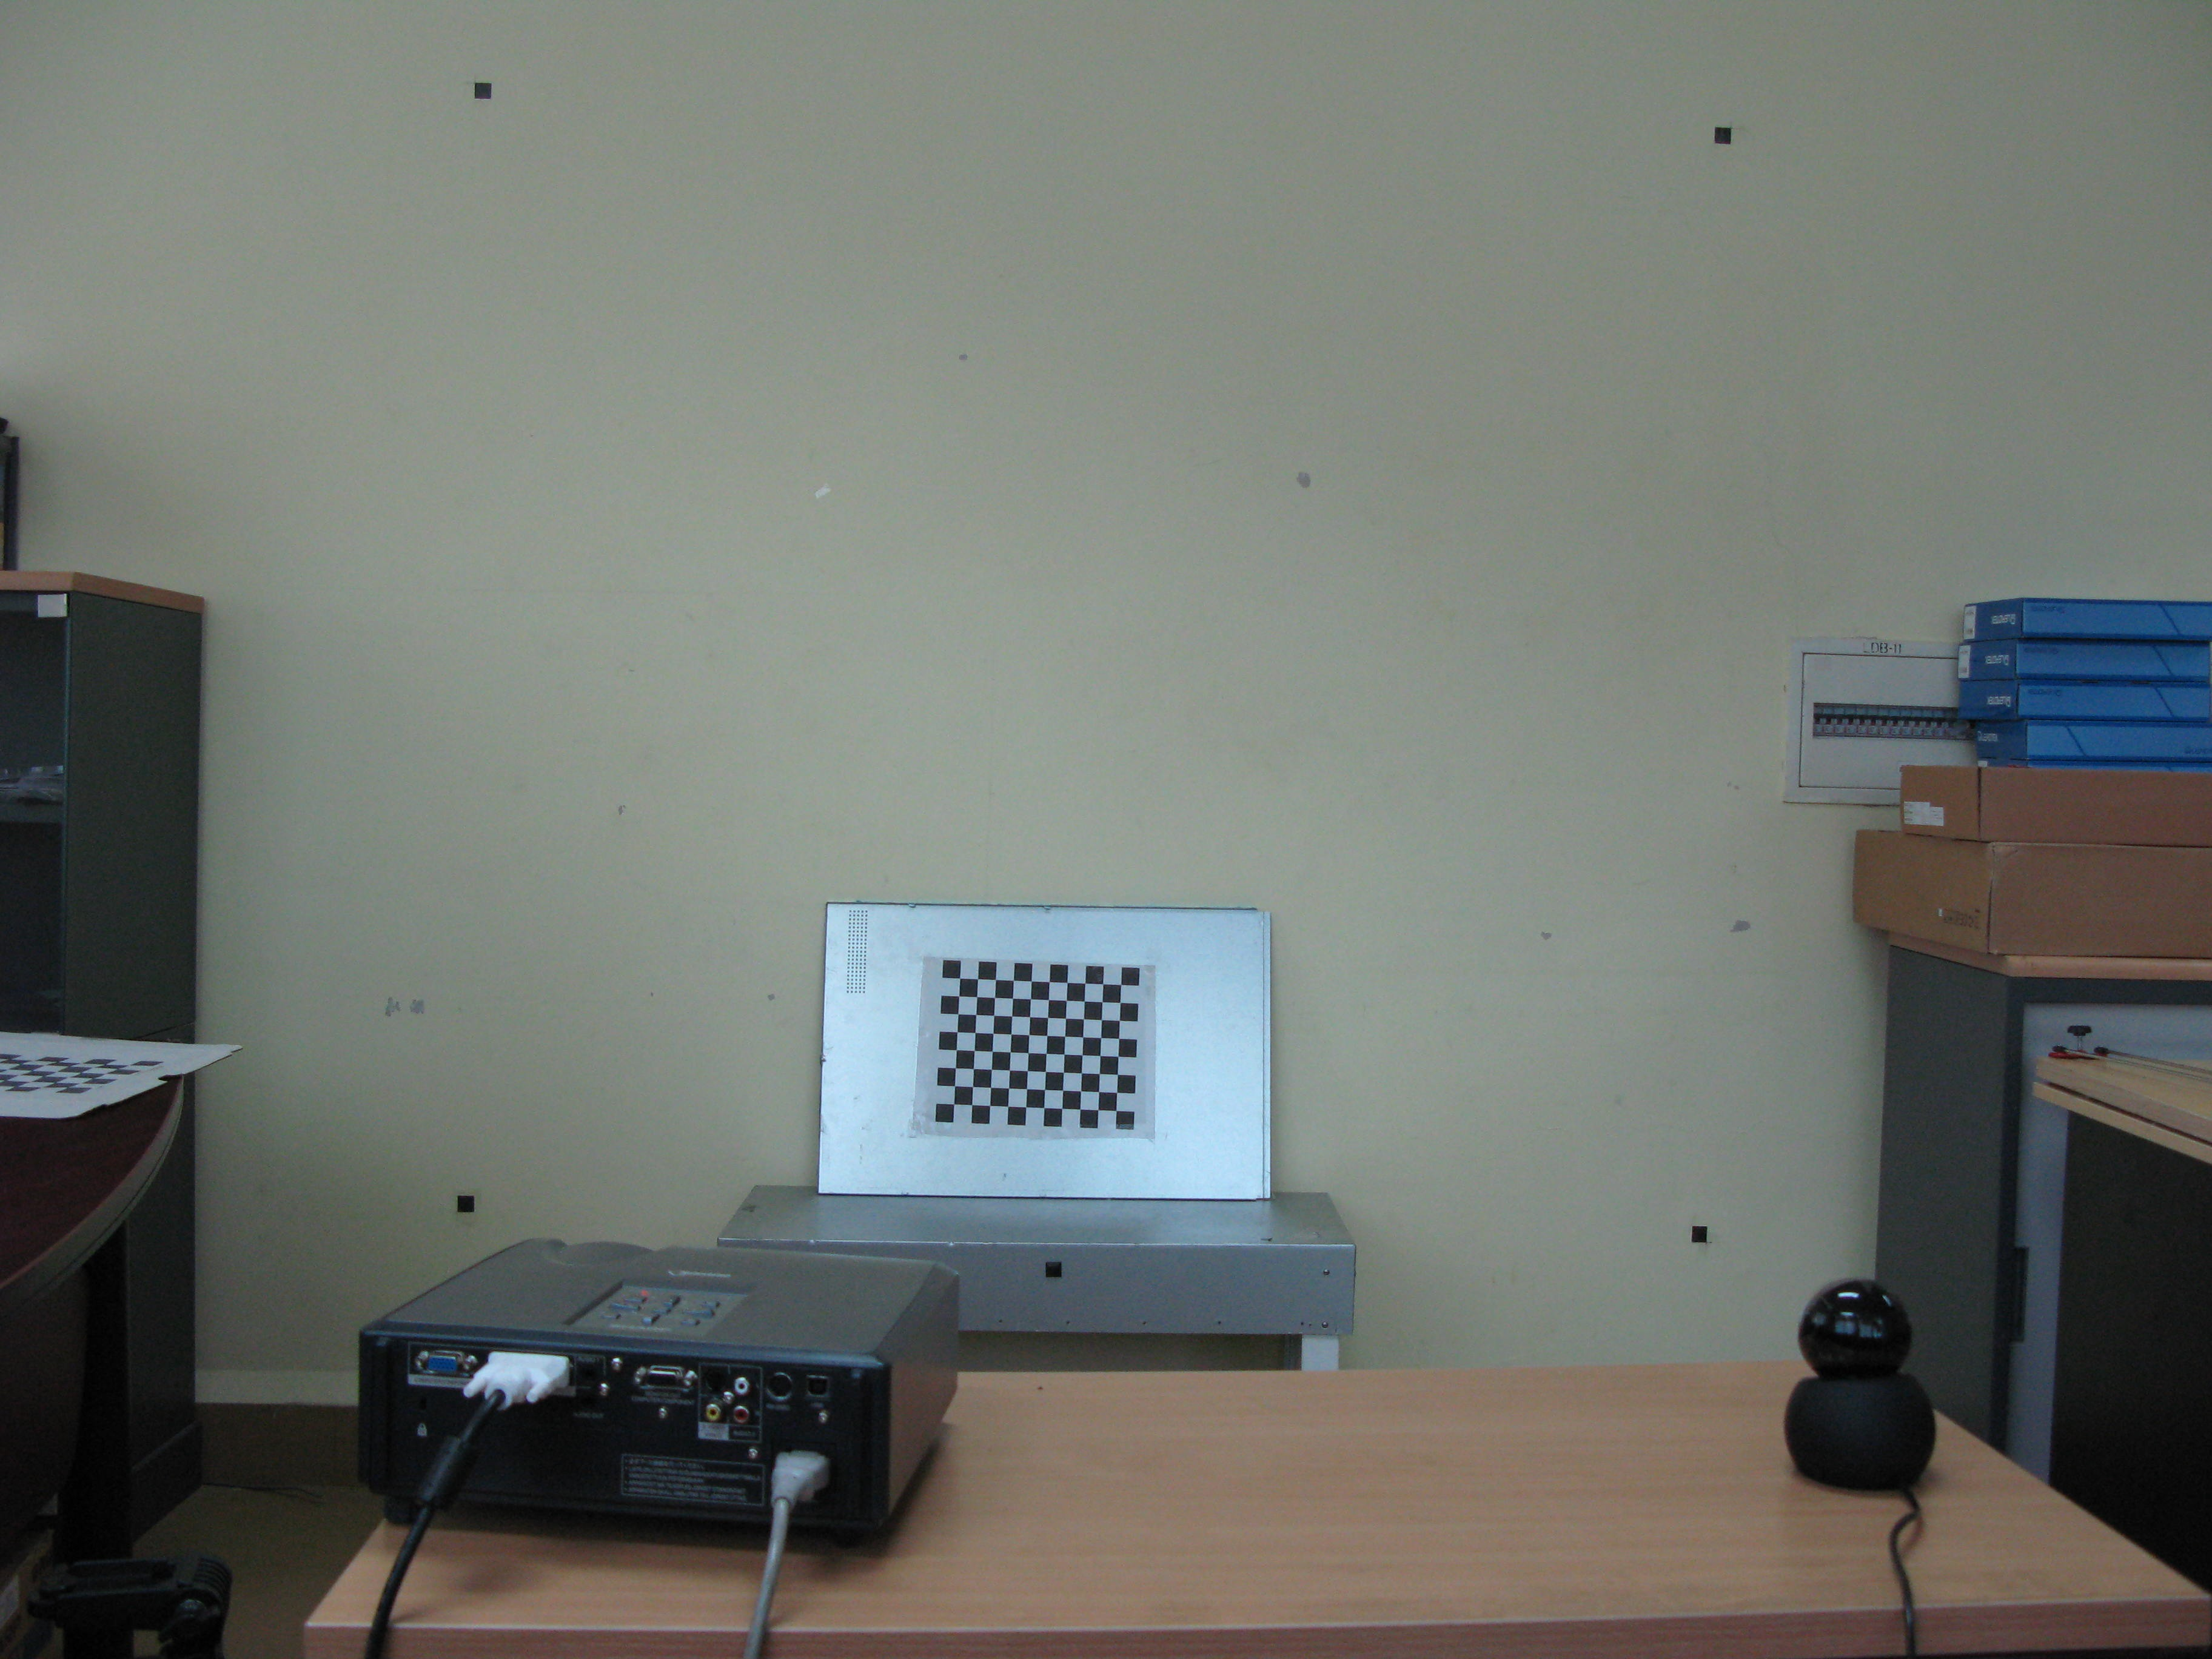
\includegraphics[width=10cm,height=8cm]{../img_source/system_setup.jpg}  
\caption{System setup}
\label{fig:calib_setup}  
\end{figure}  
  
\subsection{Camera calibration}  
In this work, camera calibration was performed using OpenCV camera calibration function whose theoretical foundations were laid by the well known algorithms by [10] and [17]. Basic overview of algorithm was presented in Section-2.3.OpenCV estimates 9 intrinsic parameters to define internal geometry of camera and 6 extrinsic parameters to define external geometry of camera with respect to world coordinate system.\newline  
\textbf{Intrinsic and distortion parameters}\newline  
$f_x$: focal length of camera lens expressed in number of pixels along X - axis\newline  
$f_y$: focal length of camera lens expressed in number of pixels along Y - axis\newline  
$(c_x , c_y)$: Pixel coordinates of principal point\newline  
$(k_1, k_2, k_3)$: Radial distortion coefficients\newline  
$(p_1,p_2)$: Tangential distortion coefficients\newline  
\textbf{Extrinsic parameters}\newline  
$(r_x,r_y,r_z)$: Rotation vector between camera and world coordinate system\newline  
$(t_x,t_y,t_z)$: Translation vector between camera and world coordinate system  
\paragraph{Procedure:}  
Aim of this process is to acquire 3D-2D correspondences between world coordinate  
system and camera image coordinate system which are then used to estimate intrinsic and  
extrinsic parameters of camera. World coordinate system origin is assumed to be at top-left corner  
of the physical checkerboard although it can be at any arbitrary position. Please note that this coordinate system origin is different from the world coordinate origin used for measurement(i.e., a corner on wall) described earlier.\newline  
\noindent  
Multiple views of the checkerboard are captured by camera and inner corners are  
detected with sub-pixel accuracy. Figure~\ref{fig:cam_calib_views} shows some such views used.\newline  
\begin{figure}[htbp]  
\centering  
\def\tabularxcolumn#1{m{#1}}  
\begin{tabularx}{\linewidth}{@{}cXX@{}}  
\begin{tabular}{c c c c}  
\hspace{0.8cm}
\subfloat[]{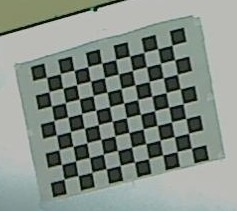
\includegraphics[width=3cm,height=3cm]{../img_source/cam_1.jpg}} &  
\subfloat[]{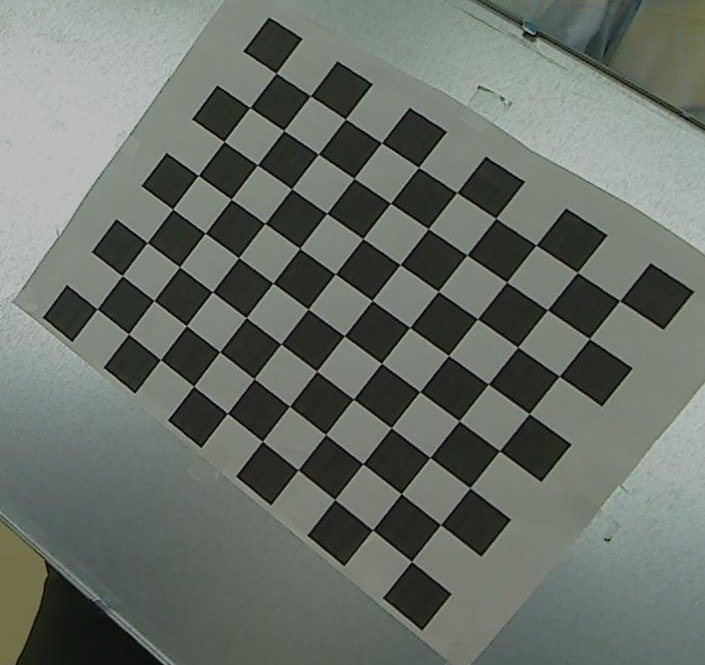
\includegraphics[width=3cm,height=3cm]{../img_source/cam_2.jpg}} &  
\subfloat[]{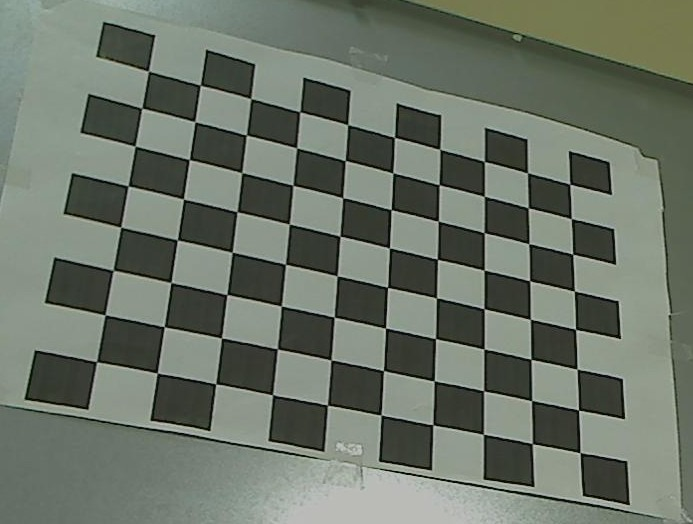
\includegraphics[width=3cm,height=3cm]{../img_source/cam_3.jpg}} &  
\subfloat[]{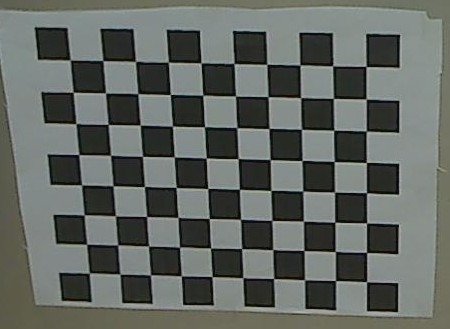
\includegraphics[width=3cm,height=3cm]{../img_source/cam_4.jpg}}\\  
\end{tabular}  
\end{tabularx}  
\caption{Some views used for camera calibration}  
\label{fig:cam_calib_views}
\end{figure}  
Each such view provides a set of 3D-2D correspondence and adds a separate set of rotation and translation parameters to the  
list of unknowns. Since there are 15 unknowns parameters per view hence at least 15 equations needs to be solved for the unknowns. This requires at least 2 views since a single view can provide only 8 constraints(i.e., 4 points are required to completely define a homography). Practically, we use more than 2 views(typically greater than 10) with more than  
4 points per view to account for effect of noise in corner-detection. Acquired 3D-2D point  
correspondences are used to calibrate camera as explained in Section-2.3.  
  
\paragraph{Results and visualization.}  
For visualization of camera calibration process a program to plot the  
views used for calibration was developed. This visualization is similar to [18] but it was not available  
for projector calibration.\newline  
Figures~\ref{fig:cam_calib_plot_1},~\ref{fig:cam_calib_plot_2} show snapshots of 3D plot of all views of checkerboard used for camera  
calibration.  
\noindent  
Here, figure~\ref{fig:cam_calib_plot_1} shows that our calibration range was 50cm to 250cm along Z-axis, -25cm to +45cm along Y-axis.  
\begin{figure}[htbp]  
\centering  
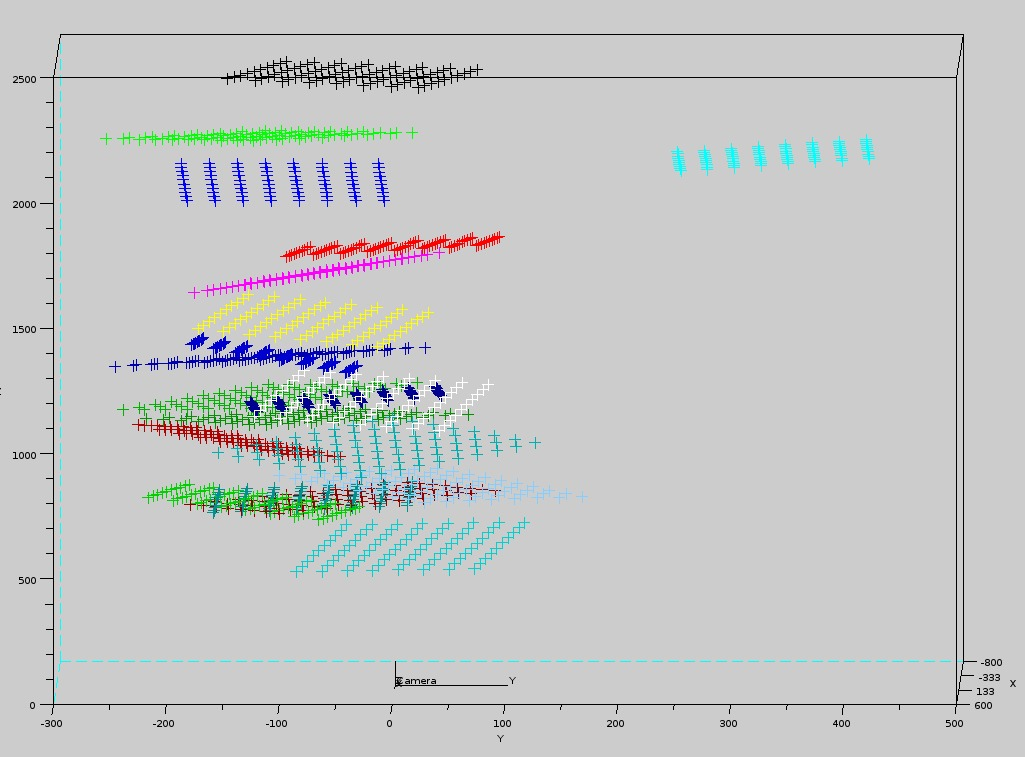
\includegraphics[width=15cm,height=10cm]{../img_source/cam_calib_view.jpg}  
\caption{Visualization of camera calibration results:View along X-axis}  
\label{fig:cam_calib_plot_1}
\end{figure}  
\noindent  
Figure~\ref{fig:cam_calib_plot_2} shows that calibration range along X-axis  
was -50cm just above +40cm. All above mentioned distances are with respect to  
camera coordinates system, which is at (0,0,0) in both figures. So the camera  
calibration volume was approximately 90cm X 70cm X 200cm.  
\begin{figure}[htbp]  
\centering  
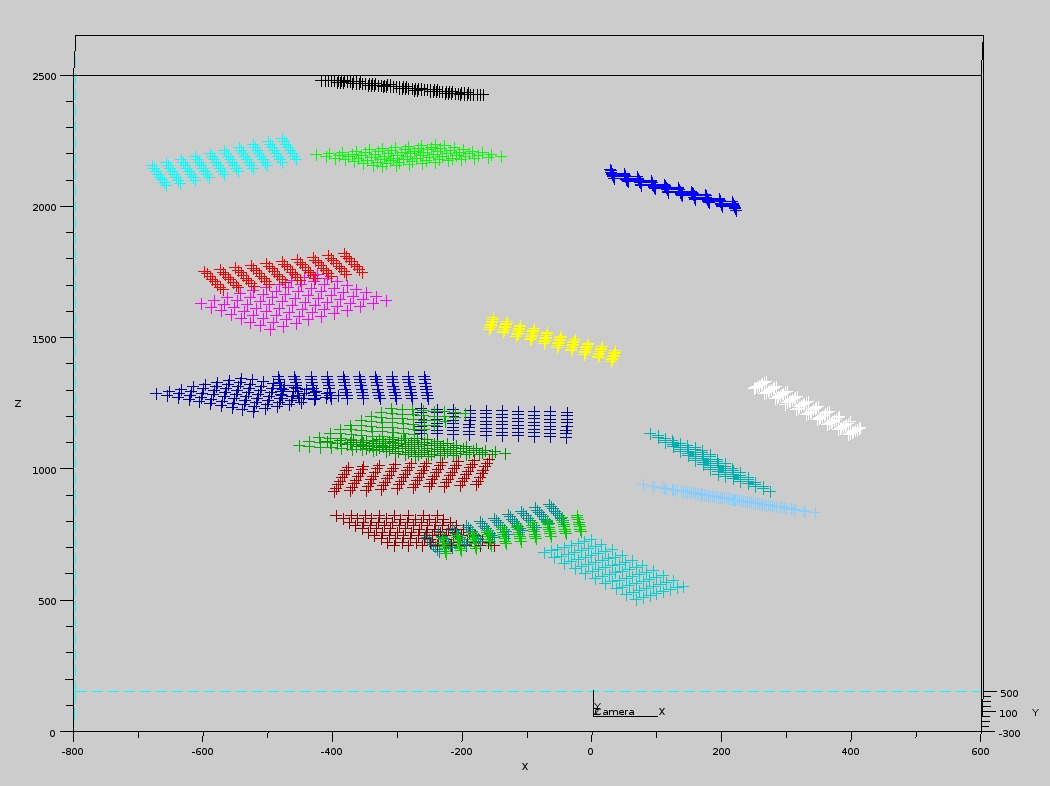
\includegraphics[width=15cm,height=10cm]{../img_source/cam_calib_view2.jpg}  
\caption{Visualization of camera calibration results:View along Y-axis} 
\label{fig:cam_calib_plot_2} 
\end{figure}  
Camera calibration parameters estimated through experiments for Logitech Quickcam sphere AF webcam at native resolution are tabulated in table 2-1. \textit{Reprojection error} mentioned in the table can be defined as a measure of deviation of fitted parameters from the observed world-camera point correspondences.% More formally,  
%\paragraph{Reprojection error.}  
%A measure of accuracy of fitted camera parameters. This is a geometric error, which quantitatively represents the euclidean distance between actual projection of a 3D point(the detected corners) and its projection computed using the estimated parameters.
\begin{table}[hb]  
\centering  
\begin{tabular}{c c}  
\hline\noalign{\smallskip}  
Parameter & Estimated value \\  
\noalign{\smallskip}\hline\noalign{\smallskip}  
$f_x$ & 1362.2\\  
$f_y$ & 1372.2\\  
$c_x$ & 803.9\\  
$c_y$ & 590.1\\  
$k_1$ & 0.07\\  
$k_2$ & -0.14\\  
%$k_3$ & 0.0\\  
%$p_1$ & 0.0\\  
%$p_2$ & 0.0\\  
Reprojection error & 0.20 \\  
\noalign{\smallskip}\hline  
\end{tabular}  
\caption{Estimated Camera intrinsic and distortion model parameters}  
\end{table}   
\subsection{Projector calibration}  
As already mentioned in Section-2.1, projector calibration problem can be regarded as an inverse-camera calibration problem. Consequently, same procedure as of camera calibration has been used to calibrate the projector. Basically, the idea is to use camera as a feedback device which will provide the 3D coordinates for the 2D features projected by the projector, hence providing the 3D-2D point correspondence between world-coordinate system and projector-coordinate system needed for projector calibration similar to camera calibration process.  
  
\paragraph{Procedure:}  
\begin{enumerate}
\item Camera-to-world homography is computed once.
\item For each view,
\begin{enumerate}
\item Projector is physically displaced allowing for rotations and translation with respect to world coordinate system and a checkerboard pattern is projected.  
\item Camera captures the projected features and detects their coordinates. 
\item Using camera-to-world homography, corresponding 3D coordinates are computed.  
\item These 3D coordinates along with the 2D coordinates of projected features(in projector buffer) forms the required 3D-2D correspondence for this view. 
\end{enumerate}
\item After sufficient number of such views(typically greater than 10) are captured projector calibration is performed using same algorithm as for camera calibration.  
\end{enumerate}
  
\noindent   
Figure~\ref{fig:proj_calib_view} shows few views used for projector calibration, projected checkerboard pattern has board dimension 11 squares X 9 squares and has each square of size of 75 pixels X 75 pixels.  
  
\begin{figure}[htbp]  
\centering  
\def\tabularxcolumn#1{m{#1}}  
\begin{tabularx}{\linewidth}{@{}cXX@{}}  
\begin{tabular}{c c c c}  
\hspace{0.8cm}  
\subfloat[]{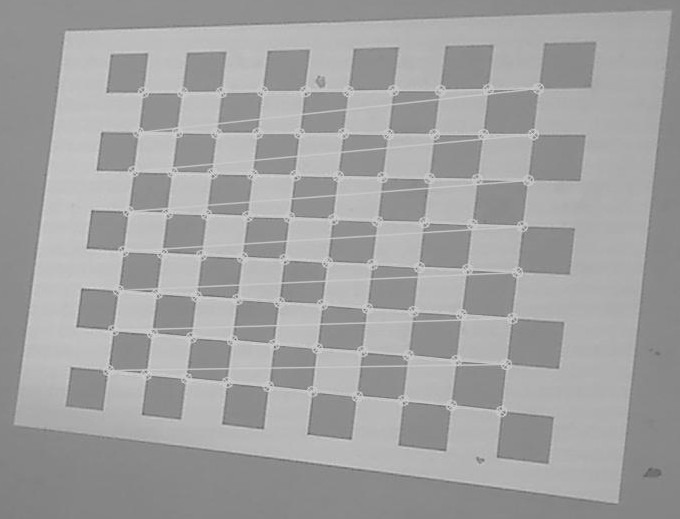
\includegraphics[width=3cm,height=3cm]{../img_source/proj_view_1.jpg}} &  
\subfloat[]{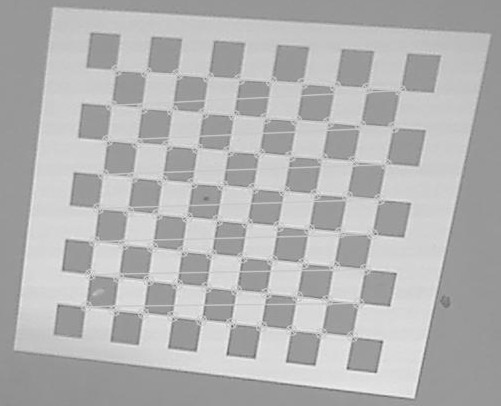
\includegraphics[width=3cm,height=3cm]{../img_source/proj_view_2.jpg}} &  
\subfloat[]{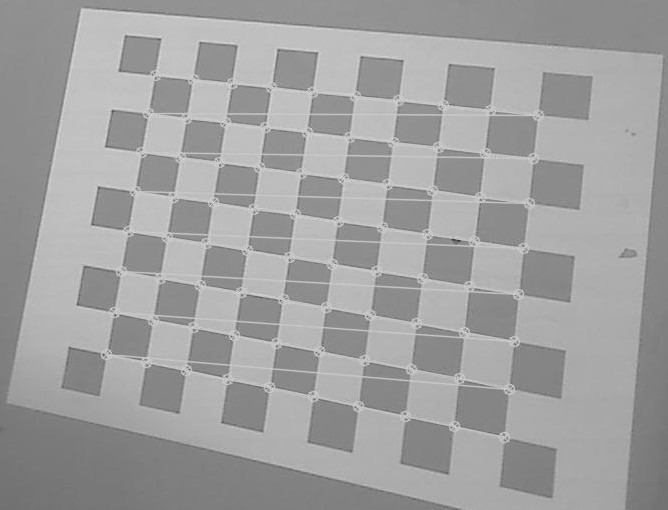
\includegraphics[width=3cm,height=3cm]{../img_source/proj_view_3.jpg}} &  
\subfloat[]{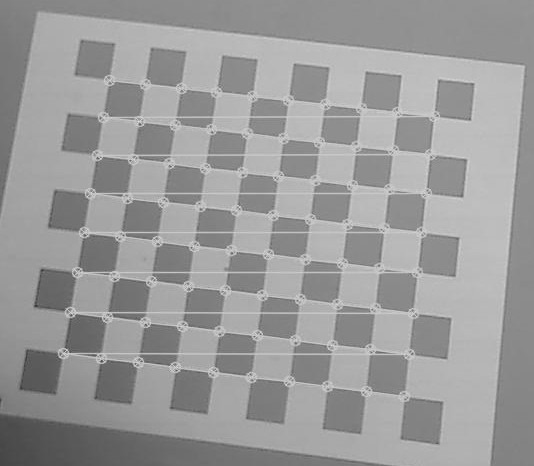
\includegraphics[width=3cm,height=3cm]{../img_source/proj_view_4.jpg}} \\  
\end{tabular}  
\end{tabularx}  
\caption{Some view used for projector calibration} 
\label{fig:proj_calib_view} 
\end{figure}  
  
  
\paragraph{Results and visualization.}  
Calibration parameters for Sharp PG F200X projector computed by performing above mentioned procedure are tabulated in table 2.2.  
\begin{table}[htbp]  
\centering  
\begin{tabular}{c c}  
\hline\noalign{\smallskip}  
Parameter & Estimated value \\  
\noalign{\smallskip}\hline\noalign{\smallskip}  
$f_x$ & 2261.7\\  
$f_y$ & 2262.8\\  
$c_x$ & 522.7\\  
$c_y$ & 713.8\\  
%$k_1$ & 0.0\\  
%$k_2$ & 0.0\\  
%$k_3$ & 0.0\\  
%$p_1$ & 0.0\\  
%$p_2$ & 0.0\\  
\noalign{\smallskip}\hline  
\end{tabular}  
\caption{Estimated Projector intrinsic model parameters}  
\end{table}  
\noindent  
Figures~\ref{fig:proj_calib_plot_1}, ~\ref{fig:proj_calib_plot_2} show plots of views used for projector calibration.Here, figure~\ref{fig:proj_calib_plot_1} shows that calibration range for along X-axis is -100cm to +150cm along Z-axis it is -50cm to +250cm.  
\begin{figure}[htbp]  
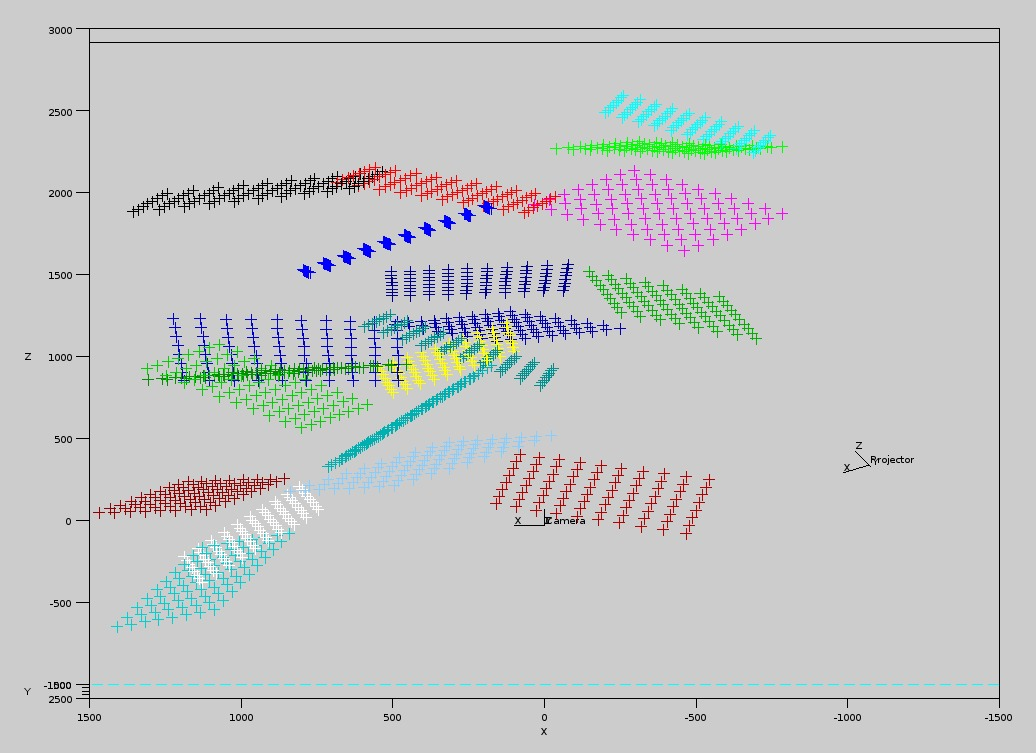
\includegraphics[width=15cm,height=10cm]{../img_source/proj_calib_plot_1.jpg}   
\caption{Visualization of projector calibration views along Y-axis} 
\label{fig:proj_calib_plot_1} 
\end{figure}  
\noindent  
Figure~\ref{fig:proj_calib_plot_2} shows calibration range along Y-axis to be from -125cm to +225cm.All measurements are with respect to camera-coordinate system which is shown at (0,0,0) in the figures. Hence calibration volume for projector was 250cm X 400cm X 300cm.  
\begin{figure}[htbp]  
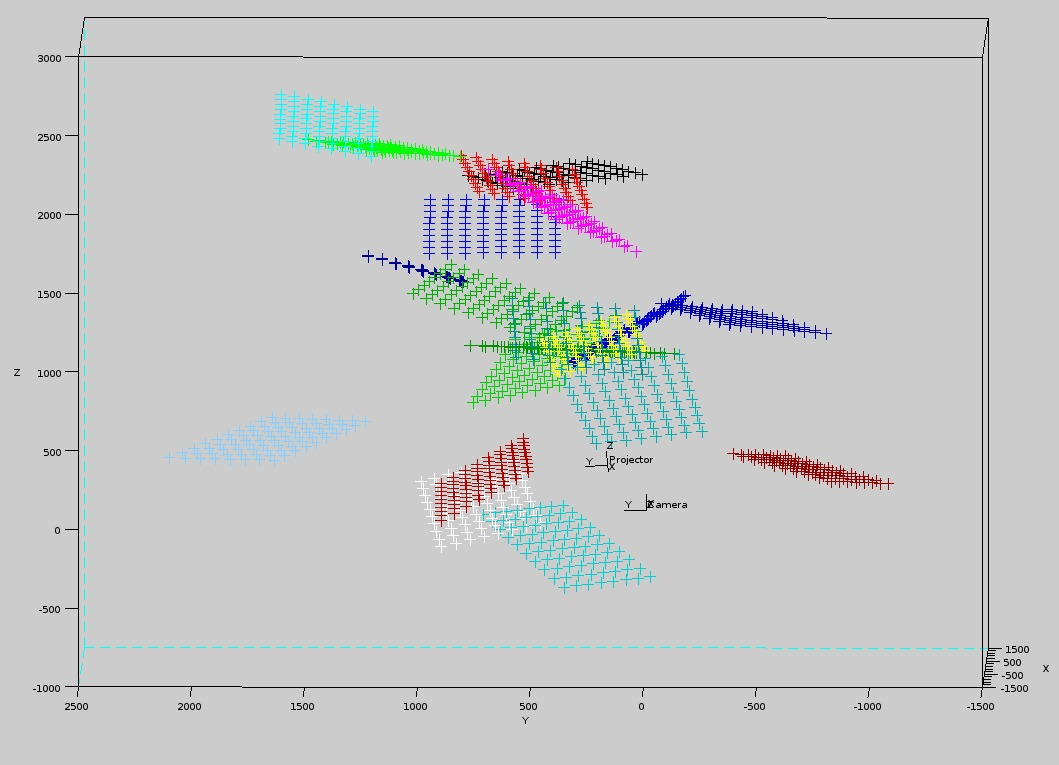
\includegraphics[width=15cm,height=10cm]{../img_source/proj_calib_plot_2.jpg}  
\caption{Visualization of projector calibration views along X-axis}  
\label{fig:proj_calib_plot_2}
\end{figure}  
  
  
  
  
  
\subsection{Camera-projector relative extrinsic calibration}   
As mentioned in an end note in section 2.3, relative calibration of projector with respect to camera is needed to bring both projector and camera to a common coordinate system which is a implicit assumption in triangulation. In this work, extrinsic calibration function available in OpenCV to determine the extrinsic parameters(i.e., rotation translation of projector coordinate system with respect to camera coordinate system) was used.  Rigid body transformations of camera and projector coordinate systems with respect to world coordinate system allow for determining the transformations between them(refer Note on relative calibration in section-2.3 for underlying equations)  
  
  
\paragraph{Procedure:}
\begin{enumerate} 
\item Extrinsic calibration of camera with respect to world coordinate system:  
\begin{enumerate}
\item A known reference plane(whose dimensions are known) containing world coordinate system is captured and corners are detected.  
\item These detected features are used for computing camera-to-world homography.  
\item Using the 3D-2D correspondences determined above, extrinsic calibration of camera is performed.  
\end{enumerate}
\item Extrinsic calibration of projector with respect to world coordinate system:  
\begin{enumerate}
\item Projector projects a checkerboard pattern, which is captured by the camera.  
\item Using the camera-to-world homography computed above, 3D coordinates for the projected feature points can be computed.  
\item These  3D-2D correspondences(3D coordinates of projected feature points and corresponding 2D coordinates in projector image) are used for computing relative rotation and translation of projector coordinate system with respect to world coordinate system.  
\end{enumerate}
\item Relative rotation and translation of projector coordinate system with respect to camera coordinate system is computed(refer Note on relative calibration in section 2.3 for underlying equations)  
\end{enumerate}  
  
\paragraph{Results and visualization.}  
Estimated extrinsic calibration parameters for a sample camera-projector geometry are tabulated in table 2.3,2.4,2.5.It should be noted however that these results are for one specific system configuration and do not represent any intrinsic characteristic of system. Hence they are called extrinsic parameters.\newline  

 
In tables~\ref{table:cam_extrinsics}.~\ref{table:proj_extrinsics},~\ref{table:cam_proj_extrinsics},  
$(r_1^{wc},r_2^{wc},r_3^{wc})$ is rotation transformation from world coordinate system to camera coordinate system  
$(t_1^{wc},t_2^{wc},t_3^{wc})$ is translation transformation from world coordinate system to camera coordinate system  
$(r_1^{wp},r_2^{wp},r_3^{wp})$ is rotation transformation from world coordinate system to projector coordinate system  
$(t_1^{wp},t_2^{wp},t_3^{wp})$ is translation transformation from world coordinate system to projector coordinate system  
$(r_1^{pc},r_2^{pc},r_3^{pc})$ is rotation transformation from projector coordinate system to camera coordinate system  
$(t_1^{pc},t_2^{pc},t_3^{pc})$ is translation transformation from projector coordinate system to camera coordinates system. Rotation vectors are expressed in radians in axis-angle form, translation is expressed in `mm'.\newline  
\begin{table}[ht]  
\parbox{.45\linewidth}{  
\centering  
\begin{tabular}{c c}  
\hline\noalign{\smallskip}  
Parameter & Estimated value \\  
\hline  
$r_1^{wc}$ & 0.128 \\  
$r_2^{wc}$ & 0.239 \\  
$r_3^{wc}$ & 0.035\\  
$t_x^{wc}$ & -920.7\\  
$t_y^{wc}$ & -834.6\\  
$t_z^{wc}$ & 2960.6\\  
\hline  
\end{tabular}   
\caption{Estimated camera extrinsic parameters}
\label{table:cam_extrinsics}
}  
\hfill  
\parbox{.45\linewidth}{  
\centering  
\begin{tabular}{c c}  
\hline\noalign{\smallskip}  
Parameter & Estimated value \\  
\hline  
$r_1^{wp}$ & -0.047 \\  
$r_2^{wp}$ & -0.246 \\  
$r_3^{wp}$ & 0.008\\  
$t_x^{wp}$ & -1054.0\\  
$t_y^{wp}$ & -1235.0\\  
$t_z^{wp}$ & 2281.0\\  
\hline  
\end{tabular}  
\caption{Estimated projector extrinsic parameters}  
\label{table:proj_extrinsics}
}\\  

\parbox{.45\linewidth}{
\centering  
\begin{tabular}{c c}  
\hline\noalign{\smallskip}  
Parameter & Estimated value \\  
\hline  
$r_1^{pc}$ & -0.086 \\  
$r_2^{pc}$ & 0.484 \\  
$r_3^{pc}$ & 0.006\\  
$t_x^{pc}$ & -1080.3\\  
$t_y^{pc}$ & 188.9\\  
$t_z^{pc}$ & 359.4\\  
\hline  
\end{tabular}  
\caption{Estimated projector-camera relative parameters}  
\label{table:cam_proj_extrinsics}
}  
\end{table}  
  
\noindent  
View used for extrinsic calibration of projector camera system is depicted in Figure~\ref{fig:extrinsic_calib_setup}. Figure~\ref{fig:extrinsic_plot} shows the plan-view of estimated projector-camera-world configuration.In figure~\ref{fig:extrinsic_plot} `green' object is the top-view of projected checkerboard. Estimated positions of world-coordinate system, projector-coordinate system and camera-coordinate system are also shown.   
\begin{figure}[htbp]  
\centering  
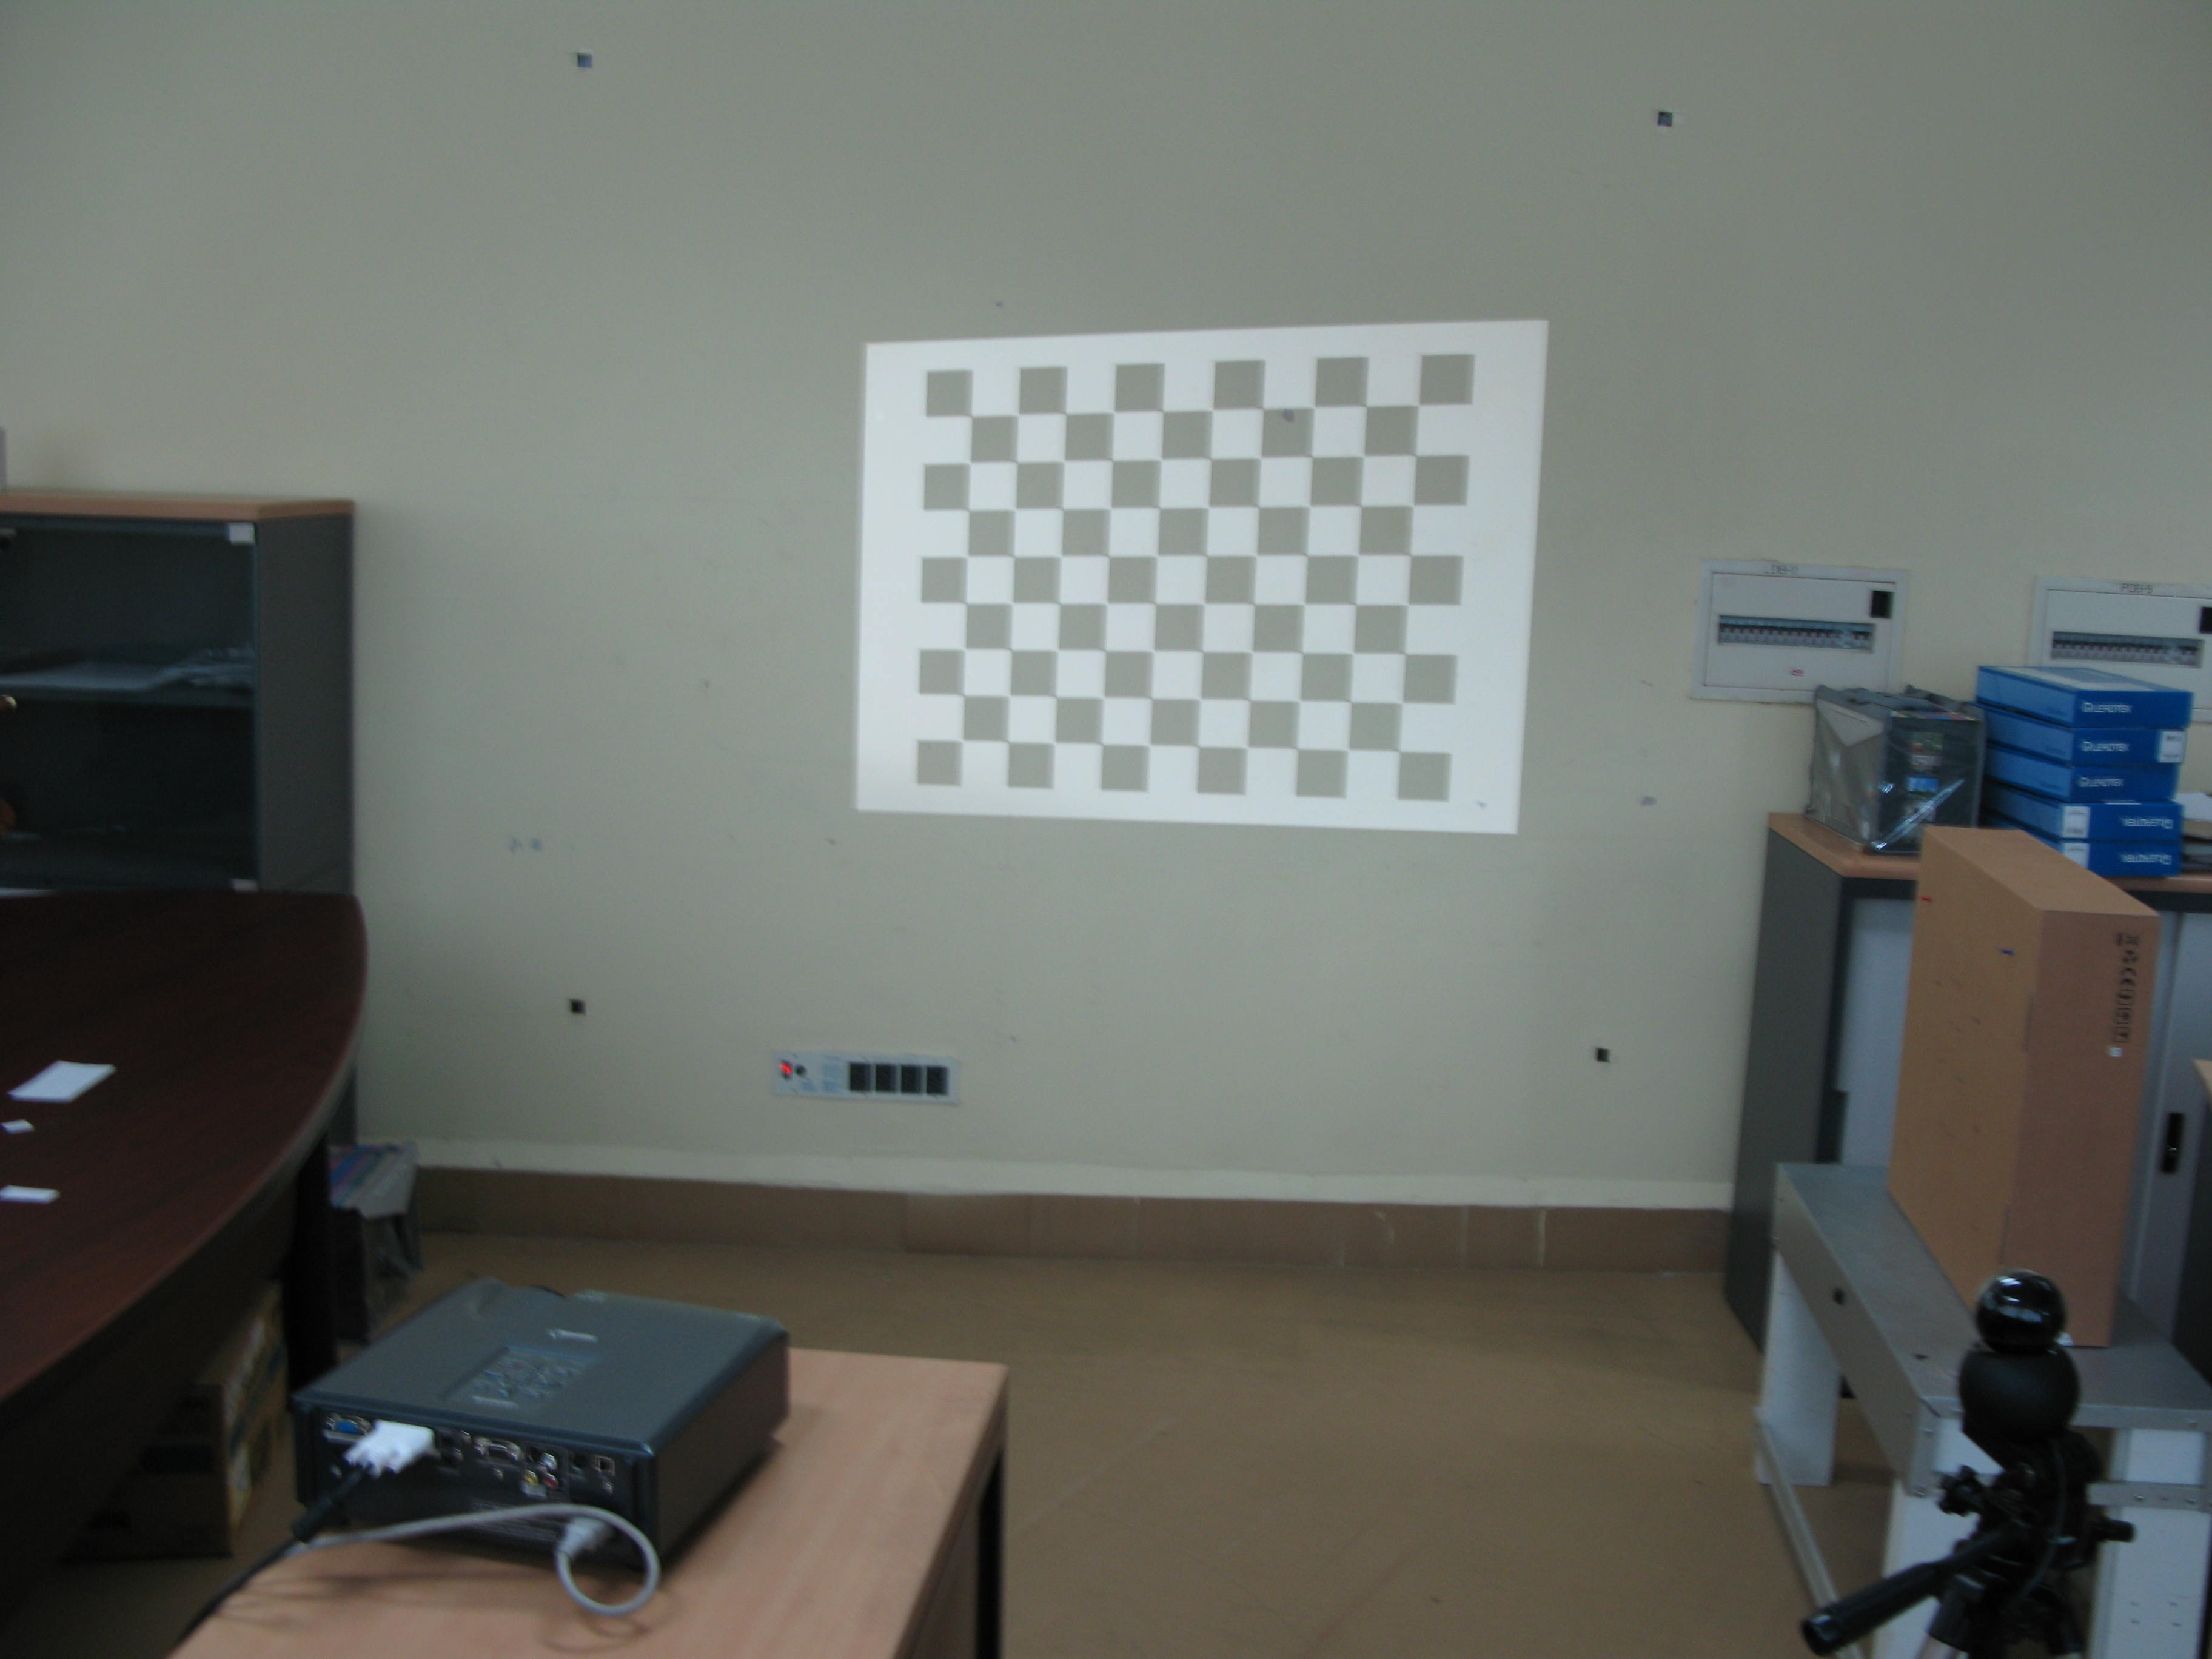
\includegraphics[width=7cm,height=5.5cm]{../img_source/system_extrinsic.jpg}  
\caption{Actual setup for extrinsic calibration}  
\label{fig:extrinsic_calib_setup}
\end{figure}  
  
\begin{figure}[!htbp]  
\centering  
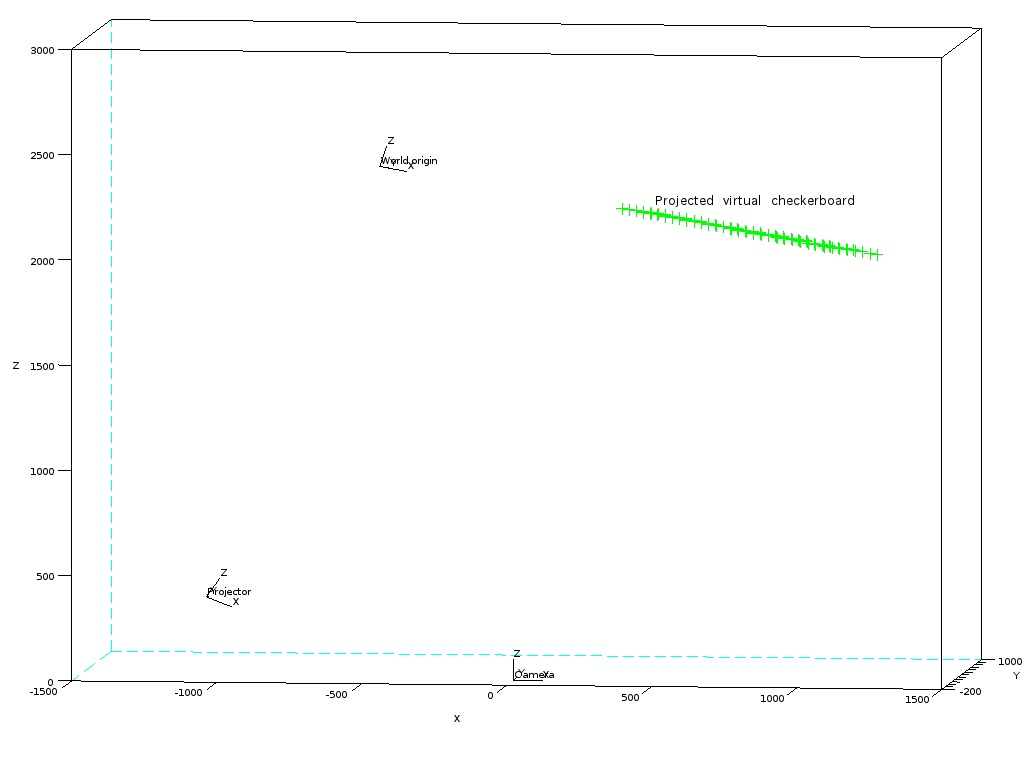
\includegraphics[width=17cm,height=11.3cm]{../img_source/system_plot_edit.jpg}  
\caption{Estimated system extrinsic geometry}  
\label{fig:extrinsic_plot}
\end{figure}  
\noindent  
 
  
\section{Discussion}  
During camera calibration it was observed that for larger distances($\sim2m$) of calibration board from camera, sub-pixel corner detection algorithm gives inaccurate results. Further, there has been no study on optimal \textit{window size} and \textit{termination criteria} for sub-pixel corner detection algorithm in the literature due to which these parameters were decided experimentally.\newline  
\indent Projector calibration using OpenCV camera calibration algorithm gives non-repeat-able estimated parameters of which reason is still unknown and deserves further study.\newline  
\indent It was observed that there are certain camera-projector geometric configurations for example when base-line between optical centers of camera and projector is small, for which OpenCV pose-estimation gives degenerate results, again this problem needs further study.   
  
  
\section{Summary}  
In this chapter, camera model was described as a series of transformations on a real world 3D point. In review, currently most popularly used calibration algorithms were briefly described. Further, working of the developed system calibration module was described with individual explanations of used procedure for camera, projector and relative extrinsic calibration. To make calibration results more comprehensive, individual plots for camera, projector and relative extrinsic calibration process were presented.
 


%% This is an example first chapter.  You should put chapter/appendix that you
%% write into a separate file, and add a line \include{yourfilename} to
%% main.tex, where `yourfilename.tex' is the name of the chapter/appendix file.
%% You can process specific files by typing their names in at the 
%% \files=
%% prompt when you run the file main.tex through LaTeX.
\chapter{Stereo correspondence}
\section{Overview of correspondence problem}
As described earlier,correspondence problem involves determining point-to-point relationship between 2 views but since these views come from projective elements like cameras,projectors,a pixel-to-pixel relation between this pair(called binocular-pair or stereo-pair) must be determined. In nutshell,establishing correspondence(technically called stereo-correspondence) means to know for a point in 3D world,which pixel in camera \& in projector(or another camera) will see it. Following section gives introduction to the current state-of-art in field of stereo-correspondence.

\section{State-of-art approaches}
To solve shape-acquisition problem following classification has been reported in literature[23][24]:\newline
1.Contact techniques:\newline
\indent   1.1 Non-destructive techniques:\newline
\indent \indent         1.1.1 Coordinate measurement machines\newline
\indent \indent         1.1.2 Jointed arms\newline
\indent   1.2 Destructive techniques:\newline
\indent \indent         1.2.1 Slicing\newline
2 Non-contact techniques:\newline
\indent   2.1 Transmissive techniques:\newline
\indent \indent          2.1.1 Industrial CT\newline
\indent   2.2 Reflective techniques:\newline
\indent \indent         2.2.1 Optical techniques:\newline
\indent \indent \indent                  2.2.1.1 Active techniques:\newline
\indent \indent \indent \indent                 2.2.1.1.1 Active stereo\newline
\indent \indent \indent \indent                 2.2.1.1.2 Imaging radar\newline
\indent \indent \indent \indent                 2.2.1.1.3 Active depth from defocus\newline
\indent \indent \indent                  2.2.1.2 Passive techniques:\newline
\indent \indent \indent \indent                 2.2.1.2.1 Passive stereo\newline
\indent \indent \indent \indent                 2.2.1.2.2 Depth from defocus\newline           
\indent \indent \indent \indent                 2.2.1.2.3 Shape from shading\newline
\indent \indent \indent \indent                 2.2.1.2.4 Shape from silhouette\newline
\indent \indent         2.2.2 Non-optical methods:\newline
\indent \indent \indent                  2.2.2.1 Microwave radar\newline
\indent \indent \indent \indent          2.2.2.2 SONAR\newline

In this work focus is on active stereo approach using structured light technique. So present survey will describe current state-of-art in structured-light techniques. Structured light systems deploy off-the-shelf video cameras \& projectors as their binocular elements. Here a camera pair of passive stereo methods is replaced by a camera-projector pair. It provides solution to the problem of correspondence for texture-less surfaces experienced by passive stereo camera pair because of lack of texture marks which act as important cues for establishing correspondence. Projection of explicit patterns which create an artificial texture on object surface,greatly simplifies the problem of correspondence. In these techniques,projector projects a pattern(s) which encode the information regarding the projector pixel which has illuminated a point in the scene. Camera captures these patterns and by decoding the pattern which is functionally equivalent to solving the correspondence problem in passive stereo vision,it extracts the unique ID of projector pixel that illuminated the same point in 3D space as is captured by camera. Figure~\ref{fig:sls}\footnote{Figure source: Refer~\cite{25}} provides conceptual representation of structured-light systems.\newline

\begin{figure}[hb]
\centering
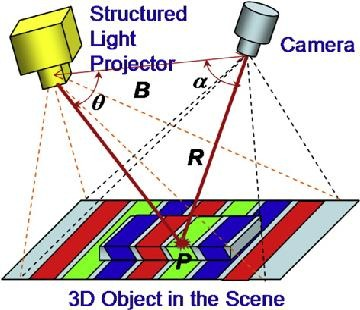
\includegraphics[width=7cm,height=7cm]{../img_source/struct_light.jpg}
\caption{A typical structured light system}
\label{fig:sls}
\end{figure}

\noindent
In figure~\ref{fig:sls},$\theta$  denotes the angle between a projector optical-ray \& baseline between camera and projector optical center.Similarly $\alpha$ denotes the angle between corresponding camera optical-ray \& baseline between camera and projector optical center.Projected pattern in the figure is just a representative of structured-light technique.\newline
\noindent
Structured light techniques have been classified in 4 major classes[23][24][26] based on how correspondence information is encoded in the projected patterns:
\paragraph{Time multiplexing.}Every point is encoded by series of intensities across multiple patterns.
\paragraph{Spatial encoding.}Every pixel is encoded based on intensities of its neighborhood pixels. 
\paragraph{Direct encoding.}Every pixel is encoded by its unique intensity and does not depend upon any spatial or temporal correlations among pixels.
\paragraph{Hybrid encoding.}It encodes pixels both spatially and temporally to project  lesser number of patterns than conventional time-multiplexing techniques and to have more robustness as compared to spatial methods.\newline \newline
\noindent
It should be noted however that this classification do not enforce unique code for each projected pixel i.e., there may be a set of pixels with same code. This pattern design decision depends upon required resolution in the reconstructed scene.

\begin{enumerate}
\item \textbf{Time multiplexing}\newline    
\noindent 
Time multiplexing techniques encode unique ID's for pixel(s) of projector over multiple patterns projected sequentially over a period of time. Camera captures all these pattern in an order to determine correct ID for each pixel(or pixel group). Depending upon type of correspondence required i.e. camera-pixel to projector-pixel or camera pixel-plane to projector pixel-number of axes of codification can be chosen to be both vertical and horizontal or one of them respectively. To be more clear, axis of codification means axis of projected pattern along which the codes are embedded other axis will simply have same copy of intensity for each code in each pattern and hence will not contribute to pixel codification. Examples of time-multiplexing based structured light patterns are binary-coded patterns, N-ary codes, gray code+phase shift method. Here i will discuss these methods as representatives for time multiplexing approach.
\begin{enumerate}
\item \textbf{Binary coded patterns} \newline
\noindent
In these patterns[27], any pixel in camera and projector is identified by the sequence of binary intensities it receives or projects respectively. Specifically, for a $N*M$ projector resolution, if pixels are to be divided into K groups along say Horizontal axis then a total of $\frac{N}{K}$ code-words will be used which will requires projection of $\log_2\lceil\frac{N}{K}\rceil$ patterns sequentially. A pattern say $j^{th}$ will represent intensities corresponding to the $j^{th}$ bit of all code-words across its horizontal axis. Hence every pattern is called a \textit{bit-plane}. Figure~\ref{fig:bin_pattern_design}\footnote{Figure source: Refer~\cite{25}} shows design of code-words, figure~\ref{fig:bin_pattern_project}\footnote{Figure source: Refer~\cite{25}} shows projection of simple binary-coded patterns scheme.After all patterns are captured by camera, a code at every pixel is computed based on intensities incident on that pixel during pattern projection. A single pattern determines single bit in code-word of all pixels in the camera image.
  

\begin{figure}
\centering
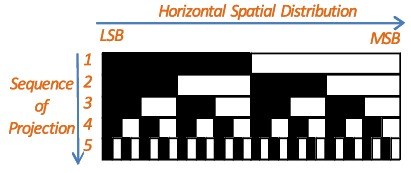
\includegraphics[width=8cm,height=5cm]{../img_source/coded_pattern_design.jpg}
\caption{Binary coded pattern:Design}
\label{fig:bin_pattern_design}
\end{figure}

\begin{figure}
\centering
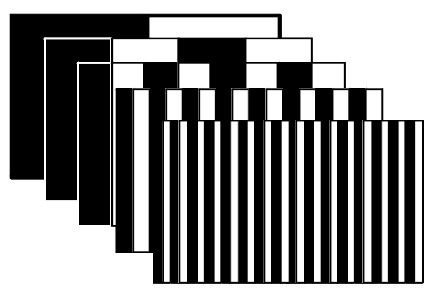
\includegraphics[width=8cm,height=5cm]{../img_source/coded_pattern_projection.jpg}
\caption{Binary coded pattern:Projection}
\label{fig:bin_pattern_project}
\end{figure}



\item \textbf{N-ary coded patterns}\newline
\noindent
In case of binary-coded patterns it can be observed that for high resolution more code-words will be required which directly increases the number of patterns to be projected. For applications requiring faster acquisition rates, number of patterns can be reduced yet meeting the resolution requirement if we increase number of intensity levels that a pixel can have[25][28][29]. This approach can allow for dynamic scene shape recovery at the cost of decreased robustness against environmental noise. As it can be deduced, color-coded patterns are special cases of this technique. Figure~\ref{fig:gray_pattern}\footnote{Figure source: Refer~\cite{25}} shows the gray-level coding scheme, here multiple allowed gray-level can be observed.

\begin{figure}[ht]
\centering
\def\tabularxcolumn#1{m{#1}}
\begin{tabularx}{\linewidth}{@{}cXX@{}}
\begin{tabular}{c c c}
\hspace{2.5cm}
\subfloat[]{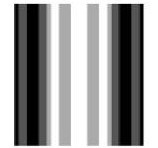
\includegraphics[width=3cm,height=3cm]{../img_source/gray_code_1.jpg}} &
\subfloat[]{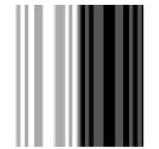
\includegraphics[width=3cm,height=3cm]{../img_source/gray_code_2.jpg}} &
\subfloat[]{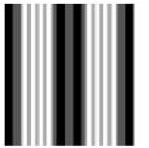
\includegraphics[width=3cm,height=3cm]{../img_source/gray_code_3.jpg}} \\
\end{tabular}
\end{tabularx}
\caption{Gray coded patterns}
\label{fig:gray_pattern}
\end{figure}

\item \textbf{Combination of gray-coded patterns and phase-shift techniques}\newline
\noindent
Gray-coded patterns were proposed to increase robustness of code recovery process against possibility of false-code extraction as compared to simple binary-coded patterns, since successive gray code-words differ at only one bit position thereby reducing chances of assigning same code to the pixels belonging to neighboring code-word groups. It has a straightforward analogy with the considerations in code designing for noisy communication channel. For a treatment of structured-light patterns in way similar to communication code designing over a noisy channel, refer[30].\newline


In phase-shift technique, phase shifted sinusoidal interference fringes are projected on object surface. In camera, unique code to each pixel is assigned in the form of phase of the signal incident on it. Similarly in projector image a phase value is assigned to each pixel which represents spatial position of that pixel in the projected sinusoidal periodic waveform. It can be deduced that this phase value indirectly encodes the position of projector pixel that projected that signal and hence the correspondence information. Figure~\ref{fig:phase_gray_method}\footnote{Figure source: Refer~\cite{25}} shows the spatially aligned combination of phase-shifted and gray coded patterns. Further details of this technique are described in section-3.4 with its actual working.\newline


Gray-coded patterns provide a way to determine a region of pixels uniquely by assigning unique code to it, whereas phase-shift technique can provide phase variation up to pixel-level within that region. Although phase-shift technique is potent to be used alone to provide pixel-level resolution but computational complexity of accurate phase value computation constraints the image resolution and scene geometry.[31] describes details of problems in accurate phase estimation called \textit{phase-unwrapping}. Hence to alleviate problem of low resolution of gray-coded patterns and computationally expensive phase-unwrapping problem, combination of both techniques is used. Here period number of a sinusoidal fringe is determined with the help of gray-coded pattern and pixel-level correspondence within that period is computed using phase-shift technique. Although it comes at a cost of increased number of patterns(typically greater than 10) that must be projected as compared to the original phase shift approach which typically requires 3 or 4 patterns. In pattern design, width of a code-word(in pixels) is equal to width of a period in phase-shifted pattern to assign a unique code-word to each fringe period and hence perform phase unwrapping. A variant of this approach is the subject of this work.

\begin{figure}[!h]
\centering
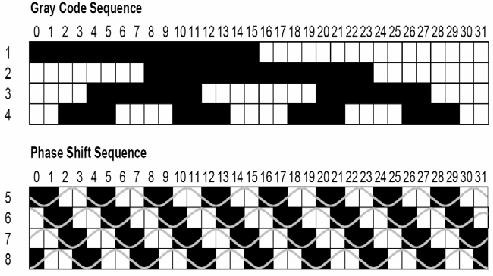
\includegraphics[width=15cm,height=8cm]{../img_source/gray+phase.jpg}
\caption{Combination of Phase-shift and gray code techniques}
\label{fig:phase_gray_method}
\end{figure}
\end{enumerate}
\item \textbf{Spatial encoding methods}\newline
As already mentioned these methods extract more information per pattern by encoding unique identity of pixels in their neighborhood(called \textit{window}) also. Although it can be clearly argued that this approach will have less robustness as compared to time-multiplexing methods since error in a decoding of one pixel will affect decoding of all dependent pixels. Here size of the window is directly proportional to the number of pixels encoded and inversely proportional to the number of intensity levels used for encoding. Basically, aim of these methods is to obtain correspondence from single captured image which facilitates them to be used for dynamic scenes(like moving objects). As can be noticed, increased number of allowed intensity-levels increases chances of error in decoding because natural scene illumination can potentially interact with these projected patterns making accurate pattern decoding more challenging than binary-coded patterns. De Bruijn patterns and M-arrays are discussed here as representatives of this technique.

\begin{enumerate}
\item \textbf{De Bruijn sequence based pattern}\newline
\noindent
De Bruijn sequence[32] of order 'm' over an alphabet of 'n' symbols is a pseudo-random sequence of length $n^m$ where every possible combination of length 'm' occurs only once. These sequences have been adapted for pattern generation by considering number of allowed intensity-level as 'n' and window length as 'm'. In terminology of graph theory it can be interpreted as a graph of $n^m$ vertices and problem of generating debruijn sequence is to determine a Hamiltonian path in that graph, this problem is also called Traveling salesmen problem. Specifically, a pattern encodes a debruijn sequence. Pattern is divided into slits where each slit has width equal to the order of the pattern. Intensities of sub-slits are generated using individual code-words occurring in debruijn sequence. Total number of intensity levels used in the pattern are limited by the alphabet size of used de-bruijn sequence. To decode a pixel it is only required to determine the code-word or window to which it belongs which will depend upon the intensities of its neighborhood pixels. Figure~\ref{fig:de_bruijn}\footnote{Figure source:~\cite{33}} shows patterns generated using debruijn sequence of various alphabets and order. 


\begin{figure}[ht]
\def\tabularxcolumn#1{m{#1}}
\begin{tabularx}{\linewidth}{@{}cXX@{}}
\begin{tabular}{lr}
\subfloat[alphabet:4,order:3]{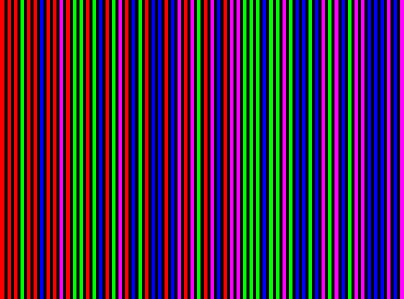
\includegraphics[width=8cm,height=3cm]{../img_source/de_bruijn_1.jpg}} &
\subfloat[alphabet:4,order:3]{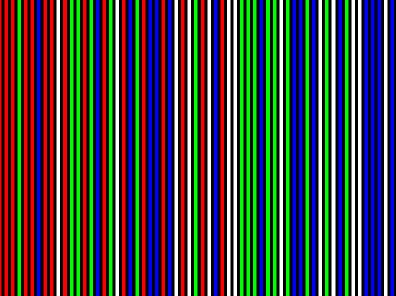
\includegraphics[width=8cm,height=3cm]{../img_source/de_bruijn_2.jpg}} \\
\subfloat[alphabet:3,order:4]{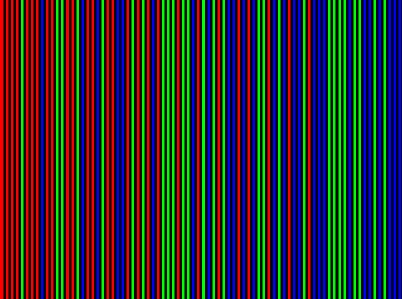
\includegraphics[width=8cm,height=3cm]{../img_source/de_bruijn_3.jpg}} &
\subfloat[alphabet:4,order:4]{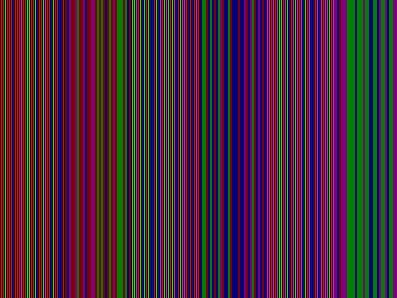
\includegraphics[width=8cm,height=3cm]{../img_source/de_bruijn_4.jpg}} \\
\end{tabular}
\end{tabularx}
\caption{De-bruijn sequence patterns}
\label{fig:de_bruijn}
\end{figure}


\item \textbf{M-array based pattern}\newline
\noindent
M-arrays[34][35] are bi-dimensional extensions of debruijn sequences. Hence a M-array of $N*M$ dimension will have all 2D code-words(in window) of dimension $W*H$ that will occur only once in complete sequence/array. One code-word will be present in one window,so it precisely means that one 2D-window will appear only once in the whole array. Figure~\ref{fig:m_array} shows a M-array based pattern.

\begin{figure}[h!]
\centering
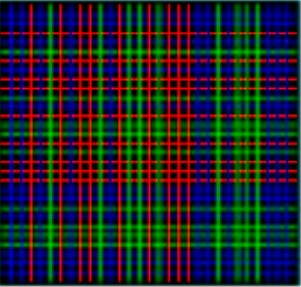
\includegraphics[width=5cm,height=5cm]{../img_source/m_array.jpg}
\caption{M-array based pattern}
\label{fig:m_array}
\end{figure}
\end{enumerate}

\item \textbf{Direct coding techniques}\newline
\noindent
In these techniques, every encoded pixel is identified by its own color/intensity. Although theoretically high resolution for dynamic scenes can be attained but practically these approach are highly susceptible to noise because of large number of intensity-levels used. It also implies that camera with very large pixel depth have to be used for detecting changes in intensity across the scene to extract code from it. Efforts in this direction include grey patterns[36][37][38] for example intensity ratio based grey pattern by [36] which fades away from black to white. Colored patterns[39][40] for example [39] proposed projection of rainbow pattern whereas [40] proposed relatively robust patterns which effectively cancels out the object color by projection of three shifted patterns but at the cost of increasing acquisition time. This approach can be classified as hybrid approach also since it includes combination of direct and temporal techniques. Figure~\ref{fig:rainbow}\footnote{Figure source: Refer~\cite{26}} shows the 3 shifted rainbow pattern as representatives of colored patterns used for direct coding techniques.

\begin{figure}[ht]
\def\tabularxcolumn#1{m{#1}}
\begin{tabularx}{\linewidth}{@{}cXX@{}}
\begin{tabular}{c c c}
\subfloat[]{
\includegraphics[width=5cm,height=5cm]{../img_source/rainbow_1.jpg}} &
\subfloat[]{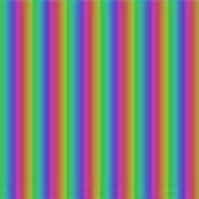
\includegraphics[width=5cm,height=5cm]{../img_source/rainbow_2.jpg}} &
\subfloat[]{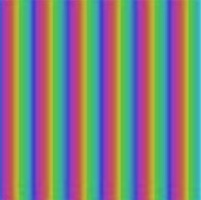
\includegraphics[width=5cm,height=5cm]{../img_source/rainbow_3.jpg}} \\
\end{tabular}
\end{tabularx}
\caption{Direct coding method:Rainbow patterns}
\label{fig:rainbow}
\end{figure}
\vspace{1.5cm}
\item \textbf{Hybrid coding techniques}\newline
\noindent
In order to attain benefits of both spatial and temporal techniques, hybrid patterns[41] were also proposed where patterns are projected temporally but their encoding also depends on neighborhood thereby allowing more information to be encoded per pattern and increased robustness from temporal technique since multiple frames contain the encoding information hence dependence on neighborhood pixels is less as compared to purely spatial neighborhood approach. This approach allowed for slow motion in the scene which is exceptional from point of view temporal-encoding schemes.
\end{enumerate}

\section{Approach followed in this work}
In this work, i have attempted to investigate the accuracy achievable by Phase-shift technique for 3D scanning since currently it is the most popular approach[42][43] for its claimed capability to achieve high accuracy and resolution in the structured-light category. It was decided to develop it also rather than just accuracy analysis because there is no \textit{open-source} implementation available for this technique except the work of [44] but it does not have documentation, is still under development and it is only for windows platform whereas we are working mainly on Linux systems. Work by [45] also attempted for three phase scanning but at the time of development had no means for system calibration and had only naive phase unwrapping algorithm which was far from being usable as a reference for accuracy analysis. \newline


Here, a combination of phase-shift technique with binary coded patterns instead of purely using phase-shifting based approach is used, reason for which is described in section-3.5. This approach gives higher spatial resolution of phase-shift technique and high noise robustness and considerable reduction in correspondence computation complexity of binary-coded patterns. Implementation details of this approach will be described in following section.   

\section{Working of developed stereo-correspondence modules}
As already shown in Figure~\ref{fig:arch}, stereo-correspondence problem is solved using a group of modules which will be described in the next subsections.

\subsection{Pattern generation}
This module allows for generation of sinusoidal interference fringe patterns of arbitrary phase shift, fringe width and binary coded patterns of arbitrary number of codewords. Binary coded patterns are generated keeping width of a sinusoid period in mind because we want to resolve among individual sinusoid periods across a pattern using binary coded patterns, so bit-width of a binary coded pattern must be equal to the period of a sinusoid. In our implementation, target was to perform ray-ray triangulation(computing intersection of corresponding optical rays from projector and camera pixels) hence we need to project horizontal and vertical versions of both fringe and binary coded patterns. Figures~\ref{fig:vert_phase_patterns} and~\ref{fig:hor_phase_patterns} show vertical and horizontal fringe patterns whereas figures~\ref{fig:vert_bin_patterns} and~\ref{fig:hor_bin_patterns} show vertical and horizontal binary coded patterns respectively. Binary coded patterns were designed using following relations:\newline

\begin{equation}
N_v^c=\frac{W_p}{w} 
\end{equation}

\begin{equation}
N_h^c=\frac{H_p}{w} 
\end{equation}

\begin{equation}
N_v^p=\log_2(N_v^c)
\end{equation}

\begin{equation}
N_h^p=\log_2(N_h^c)
\end{equation}
\noindent
where,\newline
$N_v^c$: Number of vertical binary code-words\newline
$N_h^c$: Number of horizontal binary code-words\newline
$N_v^p$: Number of vertical binary coded patterns\newline
$N_h^p$: Number of horizontal binary coded patterns\newline

\begin{figure}[htbp]
\centering
\def\tabularxcolumn#1{m{#1}}
\begin{tabularx}{\linewidth}{@{}cXX@{}}
\begin{tabular}{c c c}
\hspace{2.5cm}\subfloat[]{
\includegraphics[width=3cm,height=3cm]{../img_source/phase_ver_1.jpg}} &
\subfloat[]{
\includegraphics[width=3cm,height=3cm]{../img_source/phase_ver_2.jpg}} &
\subfloat[]{
\includegraphics[width=3cm,height=3cm]{../img_source/phase_ver_3.jpg}} \\
\end{tabular}
\end{tabularx}
\caption{Vertical phase shifted patterns}
\label{fig:vert_phase_patterns}
\end{figure}

\begin{figure}[htbp]
\centering
\def\tabularxcolumn#1{m{#1}}
\begin{tabularx}{\linewidth}{@{}cXX@{}}
\begin{tabular}{c c c}
\hspace{2.5cm}\subfloat[]{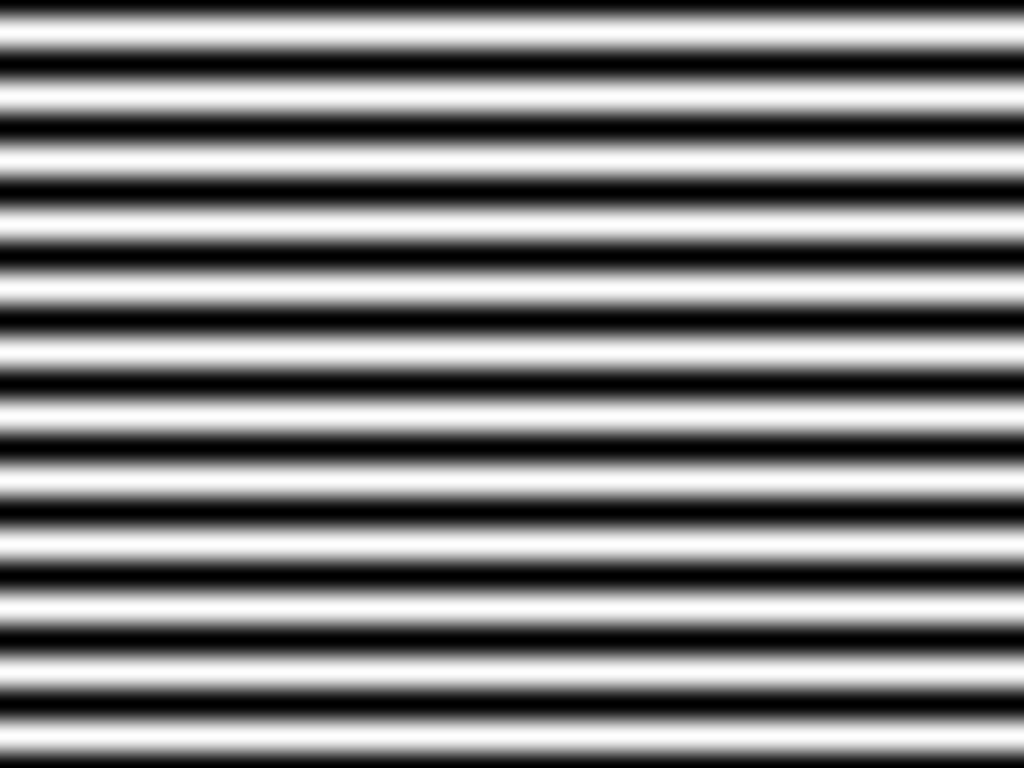
\includegraphics[width=3cm,height=3cm]{../img_source/phase_hor_1.jpg}} &
\subfloat[]{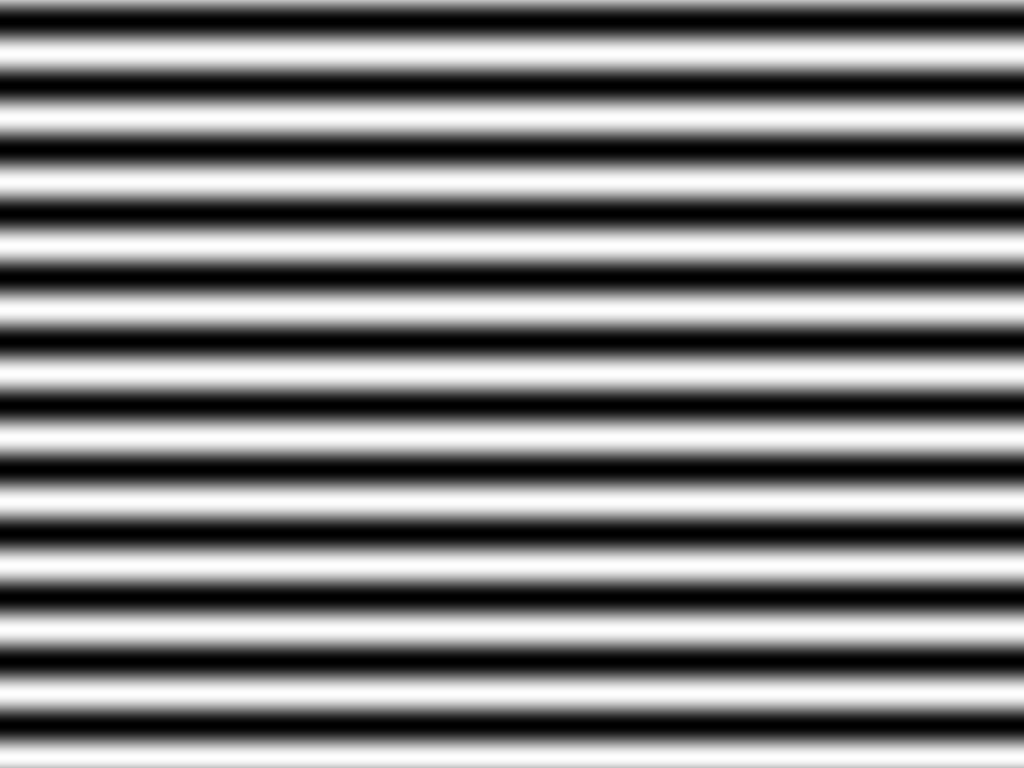
\includegraphics[width=3cm,height=3cm]{../img_source/phase_hor_2.jpg}} &
\subfloat[]{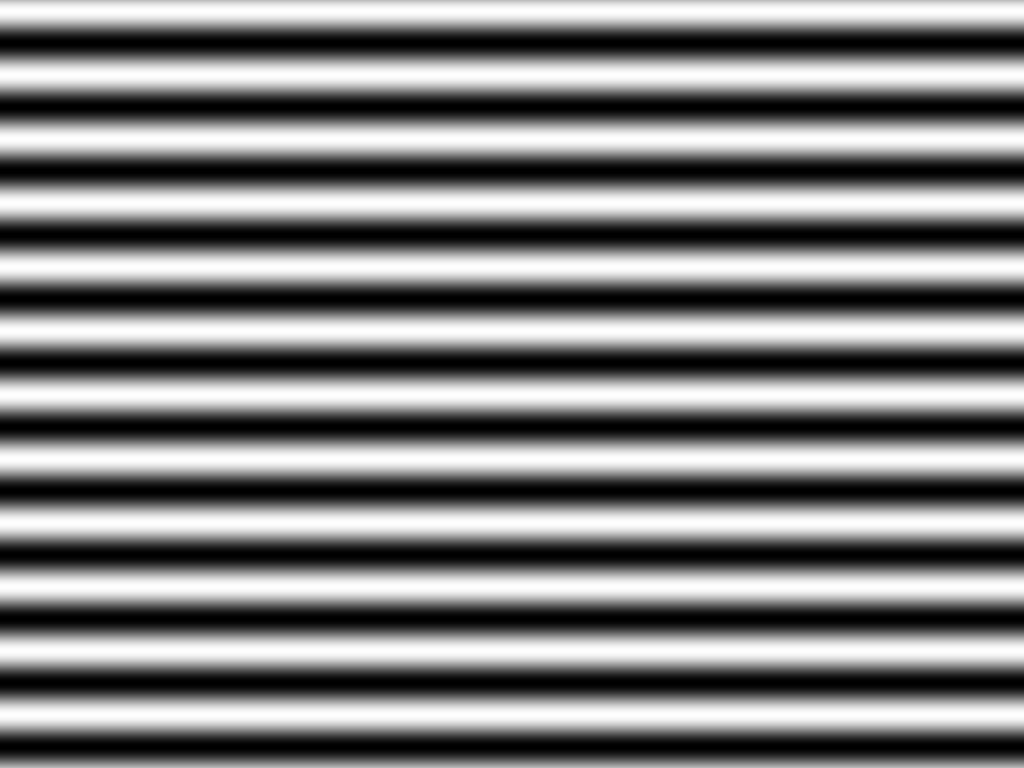
\includegraphics[width=3cm,height=3cm]{../img_source/phase_hor_3.jpg}} \\
\end{tabular}
\end{tabularx}
\caption{Horizontal phase shifted patterns}
\label{fig:hor_phase_patterns}
\end{figure}

\begin{figure}[htbp]
\centering
\def\tabularxcolumn#1{m{#1}}
\begin{tabularx}{\linewidth}{@{}cXX@{}}
\begin{tabular}{c c c}
\hspace{2.5cm}\subfloat[]{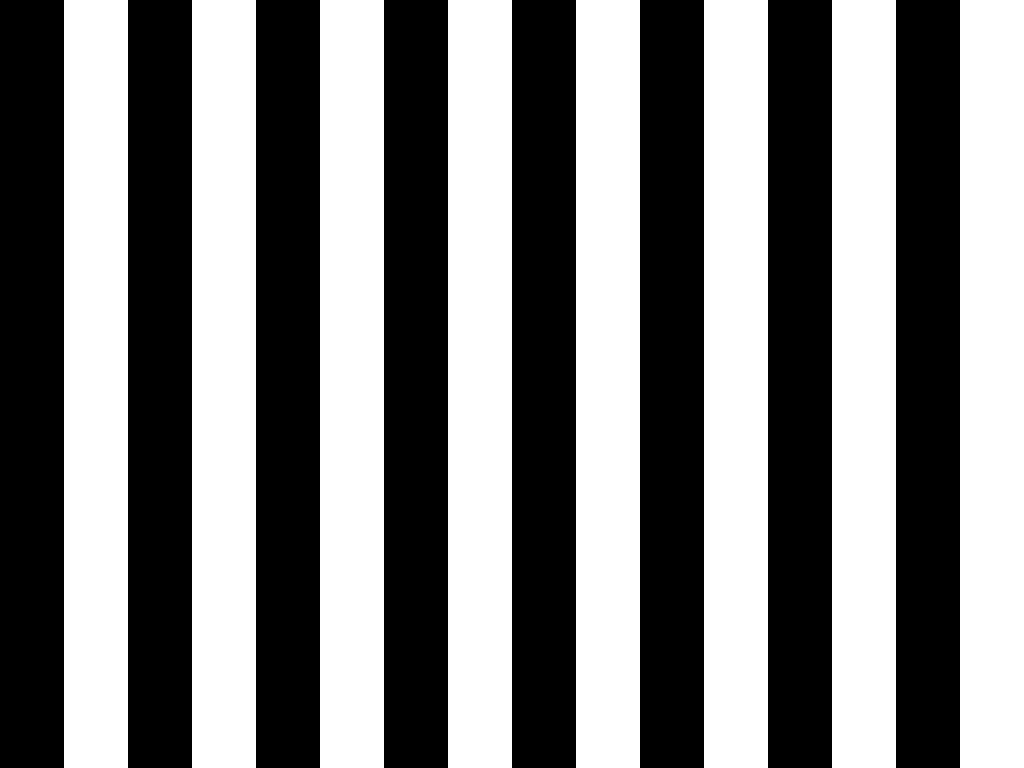
\includegraphics[width=3cm,height=3cm]{../img_source/binary_ver_1.jpg}} &
\subfloat[]{
\includegraphics[width=3cm,height=3cm]{../img_source/binary_ver_2.jpg}} &
\subfloat[]{
\includegraphics[width=3cm,height=3cm]{../img_source/binary_ver_3.jpg}} \\
\end{tabular}
\end{tabularx}
\caption{Vertical binary coded patterns}
\label{fig:vert_bin_patterns}
\end{figure}

\begin{figure}[htbp]
\centering
\def\tabularxcolumn#1{m{#1}}
\begin{tabularx}{\linewidth}{@{}cXX@{}}
\begin{tabular}{c c c}
\hspace{2.5cm}\subfloat[]{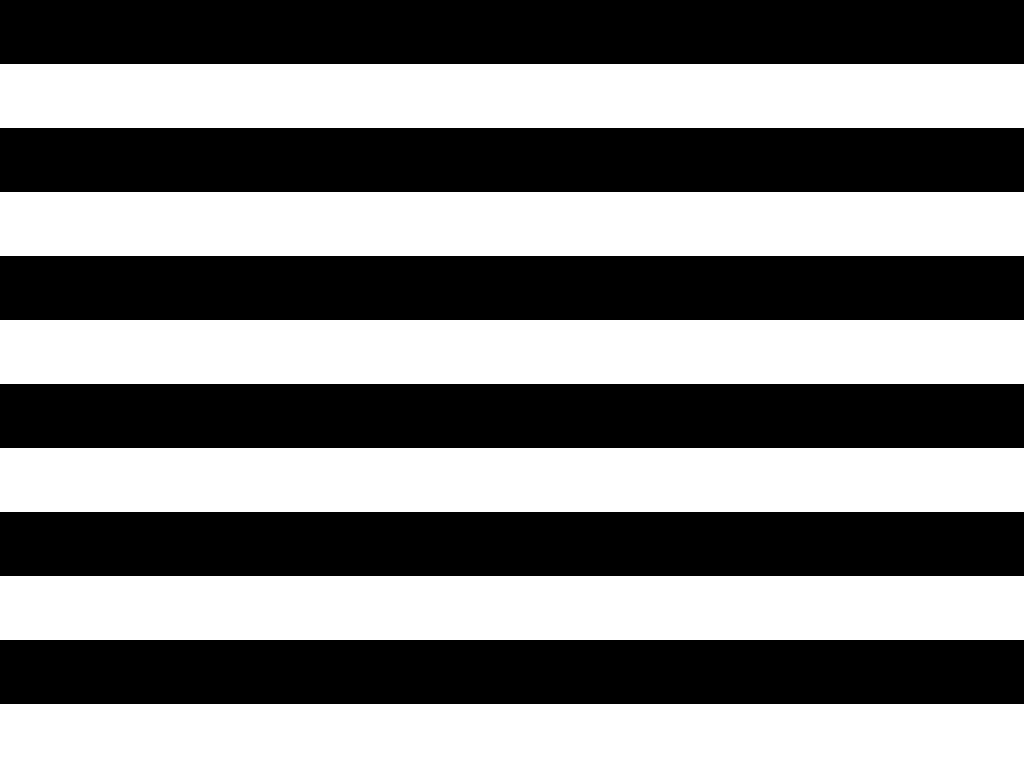
\includegraphics[width=3cm,height=3cm]{../img_source/binary_hor_1.jpg}} &
\subfloat[]{\includegraphics[width=3cm,height=3cm]{../img_source/binary_hor_2.jpg}} &
\subfloat[]{\includegraphics[width=3cm,height=3cm]{../img_source/binary_hor_3.jpg}} \\
\end{tabular}
\end{tabularx}
\caption{Horizontal binary coded patterns}
\label{fig:hor_bin_patterns}
\end{figure}


\subsection{Pattern projection and capture}
This module is developed for projection of binary coded and fringe patterns and to capture the patterns in sequential order. Currently it has only interactive control to project and capture patterns, but future version will include a synchronizing function to determine a common frequency of pattern projection and capture. In addition this module allows to control brightness of projector and camera. It allows to manipulate shutter-speed of camera hence facilitating to adapt according to varying illumination conditions. All projected and captured images are undistorted(i.e. camera/projector lens distortion effects are reduced) using the projector and camera intrinsic calibration parameters respectively. Figure~\ref{fig:capt_vert_fringe_bin} shows the captured vertical fringe and binary coded patterns. Figure~\ref{fig:capt_hor_fringe_bin} shows some captured horizontal fringe and binary coded patterns.

\begin{figure}[htbp]
\def\tabularxcolumn#1{m{#1}}
\begin{tabularx}{\linewidth}{@{}cXX@{}}
\begin{tabular}{c c c}
\hspace{1.1cm}\subfloat[]{\includegraphics[width=4cm,height=4cm]{../img_source/cap_fringe_1.jpg}} &
\subfloat[]{\includegraphics[width=4cm,height=4cm]{../img_source/cap_fringe_2.jpg}} &
\subfloat[]{\includegraphics[width=4cm,height=4cm]{../img_source/cap_fringe_3.jpg}} \\
\hspace{1.1cm}\subfloat[]{\includegraphics[width=4cm,height=4cm]{../img_source/cap_fringe_4.jpg}} &
\subfloat[]{\includegraphics[width=4cm,height=4cm]{../img_source/cap_fringe_5.jpg}} &
\subfloat[]{\includegraphics[width=4cm,height=4cm]{../img_source/cap_fringe_6.jpg}} \\
\end{tabular}
\end{tabularx}
\caption{Some captured vertical fringe and binary coded patterns}
\label{fig:capt_vert_fringe_bin}
\end{figure}
\begin{figure}[htbp]
\def\tabularxcolumn#1{m{#1}}
\begin{tabularx}{\linewidth}{@{}cXX@{}}
\begin{tabular}{c c c}
\hspace{1.1cm}\subfloat[]{\includegraphics[width=4cm,height=4cm]{../img_source/cap_binary_1.jpg}} &
\subfloat[]{\includegraphics[width=4cm,height=4cm]{../img_source/cap_binary_2.jpg}} &
\subfloat[]{\includegraphics[width=4cm,height=4cm]{../img_source/cap_binary_3.jpg}} \\
\hspace{1.1cm}\subfloat[]{\includegraphics[width=4cm,height=4cm]{../img_source/cap_binary_4.jpg}} &
\subfloat[]{\includegraphics[width=4cm,height=4cm]{../img_source/cap_binary_5.jpg}} &
\subfloat[]{\includegraphics[width=4cm,height=4cm]{../img_source/cap_binary_6.jpg}} \\
\end{tabular}
\end{tabularx}
\caption{Some captured horizontal fringe and binary coded patterns}
\label{fig:capt_hor_fringe_bin}
\end{figure}

\subsection{Phase wrapping}
Projected sinusoidal fringe pattern is periodic in nature. It implies that there exists ambiguity in determining the phase of any point across the pattern. This ambiguity is manifested in the illumination model used in Phase-shift technique. Following equations show the assumed illumination model at every camera pixel for three phase-shift technique[9] for both horizontal and vertical fringe patterns:\newline
\begin{equation}
\begin{aligned}
& I_1=I_{dc}+I_{mod}*cos(\phi-\psi) \\
& I_2=I_{dc}+I_{mod}*cos(\phi) \\
& I_3=I_{dc}+I_{mod}*cos(\phi+\psi)
\end{aligned}
\end{equation}
\noindent
where,\newline
$I_i$: Captured intensity when $i^{th}$ pattern is projected\newline
$\phi$: Wrapped phase\newline
$\psi$: Constant phase shift between successive patterns\newline
$I_{dc}$: Background intensity\newline
$I_{mod}$: Intensity modulation\newline
\noindent
Assuming $\psi=\frac{2\pi}{3}$,using this system of equations $\phi$ can be solved at every pixel as:\newline

\begin{equation}
\phi=tan^{-1}\bigg[\frac{\sqrt[2]{3}(I_1-I_3)}{2I_2-I_1-I_3}\bigg]
\end{equation}
where, $-\pi\leq\phi\leq\pi$ \newline
\noindent
Since $\phi$ lies from $-\pi$ to $\pi$, information regarding actual phase at every point is mapped to this range hence it is called \textit{wrapped phase}. It cannot be resolved for correct corresponding projector pixel unless we compute the corresponding period number. This task is performed by module described in next subsection. Figure~\ref{fig:wrapped_phase} shows the wrapped phase computed from the captured phase shifted fringe images.

\begin{figure}[htbp]
\def\tabularxcolumn#1{m{#1}}
\begin{tabularx}{\linewidth}{@{}cXX@{}}
\begin{tabular}{c c}
\hspace{2cm}\subfloat[Vertical wrapped phase]{\includegraphics[width=4.5cm,height=4cm]{../img_source/wrapped_ver.jpg}} &
\hspace{2cm}\subfloat[Horizontal wrapped phase]{\includegraphics[width=4.5cm,height=4cm]{../img_source/wrapped_hor.jpg}}\\
\end{tabular}
\end{tabularx}
\caption{Computed wrapped phase}
\label{fig:wrapped_phase}
\end{figure}

\paragraph{Extension to four and five phase shifted fringe patterns.}
In order to assess the effect of increasing the number of phase shifted patterns on accuracy of estimated stereo-correspondence,  the basic 3D scanner with 3 phase shifted patterns was extended to be able to project and process four and five phase shifted patterns also. It should be noted however that only pattern generator and phase wrapper modules need to be extended for this purpose as all remaining modules are independent of number of patterns used for 3D scanning. Further it should be pointed out that \textit{three} is the minimum number of phase shifted patterns that can be used assuming $I_{dc}$, $I_{mod}$ and $\phi$ as unknowns which requires at least 3 equations and hence 3 patterns. Equation 3-7 describes assumed illumination model for 4 phase-shifted pattern technique,  equation 3-8 expresses the corresponding wrapped phase. Whereas equation 3-9 expresses the illumination model for 5 phase shifted pattern technique and equation 3-10 represents the corresponding wrapped phase. Unknowns $I_{dc}$, $I_{mod}$, $\phi$ have same meaning as in equation 3-5,3-6.\newline
\noindent
For four sinusoidal fringe patterns phase-shifted by $\pi/2$,
\begin{equation}
\begin{aligned}
& I_0=I_{dc}+I_{mod}*cos(\phi) \\
& I_1=I_{dc}+I_{mod}*cos(\phi+\pi/2) \\
& I_2=I_{dc}+I_{mod}*cos(\phi+\pi) \\
& I_3=I_{dc}+I_{mod}*cos(\phi+3\pi/2)
\end{aligned}
\end{equation}
Simultaneously solving equations 3-7 gives wrapped phase, $\phi$ as:
\begin{equation}
\phi=tan^{-1}\bigg[\frac{I_3-I_1}{I_0-I_2}\bigg]
\end{equation}
Similarly for five sinusoidal fringe patterns phase-shifted by $2\pi/5$,
\begin{equation}
\begin{aligned}
& I_0=I_{dc}+I_{mod}*cos(\phi-4\pi/5) \\
& I_1=I_{dc}+I_{mod}*cos(\phi-2\pi/5) \\
& I_2=I_{dc}+I_{mod}*cos(\phi) \\
& I_3=I_{dc}+I_{mod}*cos(\phi+2\pi/5)\\
& I_4=I_{dc}+I_{mod}*cos(\phi+4\pi/5)
\end{aligned}
\end{equation}
Solving equations 3-9 gives wrapped phase $\phi$ as: 
\begin{equation}
\phi=tan^{-1}\bigg[2sin\alpha*\bigg(\frac{I_1-I_3}{2I_2-I_4-I_0}\bigg)\bigg]
\end{equation}


\subsection{Pixel decoding and phase unwrapping}
Periodic nature of sinusoidal interference fringes creates ambiguous condition in which multiple pixels in camera image can have same wrapped phase hence there is need to assign distinct period numbers to such candidates thereby eliminating the ambiguity. This step is called \textit{phase unwrapping}. Therefore a module to perform phase unwrapping was developed which uses information from binary code projected onto the object to recover this period number. It should be noted here that wrapped and hence unwrapped phase is computed in both vertical and horizontal directions. Hence we get a pair of unwrapped phase associated with each valid camera pixel. Here a camera pixel is called \textit{valid} if it corresponds to the region on which pattern is projected and has a Signal/Noise ratio greater than a threshold(this threshold is environment illumination dependent in current implementation).Equation 3.11 describes the criteria used as a measure of Signal/Noise ratio for 3 phase-shift approach.
\begin{equation}
\eta=\frac{I_{mod}}{I_{dc}}=\frac{\sqrt[2]{3(I_1-I_3)^2+(2I_2-I_1-I_3)^2}}{I_1+I_2+I_3}
\end{equation}
Here,$\eta$ represents the Signal/Noise ratio,hence,pixel(x,y) is \textit{valid} if $\eta(x,y)>T$,where $T$ is assumed threshold.


Unwrapped phase is calculated using information from both fringe projection and binary coded techniques as. Following equation represent represents this problem:\newline

\begin{equation}
\oint(x,y)=\phi(x,y)+2\pi*C(x,y)
\end{equation}
\noindent
where,\newline
$\oint(x,y)$: Unwrapped phase at pixel (x,y)\newline
C(x,y): Decoded binary code at pixel (x,y)\newline
\noindent
This equation is applied for both horizontal and vertical phase unwrapping. Figure~\ref{fig:unwrapped_phase} represents the unwrapped phase corresponding to the wrapped phase shown in figure~\ref{fig:wrapped_phase}.

\begin{figure}[ht]
\def\tabularxcolumn#1{m{#1}}
\begin{tabularx}{\linewidth}{@{}cXX@{}}
\begin{tabular}{l r}
\hspace{2cm}\subfloat[Vertical unwrapped phase]{\includegraphics[width=4.5cm,height=4cm]{../img_source/unwrapped_ver.jpg}} &
\hspace{2cm}\subfloat[Horizontal unwrapped phase]{\includegraphics[width=4.5cm,height=4cm]{../img_source/unwrapped_hor.jpg}}\\
\end{tabular}
\end{tabularx}
\caption{Computed unwrapped phase}
\label{fig:unwrapped_phase}
\end{figure}

\subsection{Correspondence computation using absolute phase}
Stereo-correspondence between binocular elements like a projector-camera pair relates the points in projector and camera image-space which are observing a common 3D point in the scene.\newline% Figure~\ref{fig:correspond_abstract} shows stereo-correspondence for clarity. Here a point in left view is related to a point in right view because they are 2D projections of a common point named \textit{Scene Point} in the scene using estimated stereo-correspondence.
%\begin{figure}
%\centering
%\includegraphics[width=8cm,height=8cm]{../img_source/stereo_correspondence_abstract.jpg}
%\caption{Stereo correspondence:abstract representation}
%\label{fig:correspond_abstract}
%\end{figure}
%\begin{figure}
%\begin{tikzpicture}
%\fill[green] (0,0) circle[radius=2pt];
%\draw (-3,) rectangle ();
%\end{tikzpicture}
%\end{figure}
%\noindent
\indent Once the unwrapped phase is computed,camera-projector pixel-pixel correspondences can be computed directly by searching for pixels in projector with same vertical and horizontal unwrapped phase values as that of corresponding valid camera pixel. It is computed as:
\begin{equation}
\begin{aligned}
& X_p=\lfloor w_{fringe}*\big(\frac{\oint_v(X_c,Y_c)}{2\pi}\big) \rfloor \\ 
& Y_p=\lfloor w_{fringe}*\big(\frac{\oint_h(X_c,Y_c)}{2\pi}\big) \rfloor
\end{aligned}
\end{equation}
\noindent
where,\newline
$(X_p,Y_p)$: Projector coordinates corresponding to camera coordinates $(X_c,Y_c)$\newline
$w_{fringe}$: Width of projected fringe in pixels.\newline
Figure~\ref{fig:estimated_correspondence} shows the one result of correspondence computation using the developed system.
\begin{figure}[htbp]
\def\tabularxcolumn#1{m{#1}}
\begin{tabularx}{\linewidth}{@{}cXX@{}}
\begin{tabular}{c c}
\hspace{2cm}
\subfloat[Camera image]{\includegraphics[width=4.5cm,height=4cm]{../img_source/camera_image.jpg}} &
\hspace{2cm}\subfloat[Projector image]{\includegraphics[width=4.5cm,height=4cm]{../img_source/projector_image.jpg}} 
\end{tabular}
\end{tabularx}
\caption{Stereo correspondence between camera and projector:\textit{green} spot in (b) corresponds to selected point(cursor) in (a)}
\label{fig:estimated_correspondence}
\end{figure}




\section{Discussion}
It was observed that phase-shift technique do not work well on surface with very high(or very low) surface reflectance, surface interreflections, subsurface scattering and in cases when projector or camera is/are defocused. These problems are still a limitation of structured light technique. However some developments for this problem have been reported recently[46].\newline
\indent Further, an ambiguity in decoding the binary coded patterns was observed at the edges of strips which due to projector or camera blur becomes wider \textit{grey} region which cannot be reliably judged black or white in general. Because of this problem, points in the strip region were discarded while evaluating accuracy and precision of the system.\newline
\indent Although original plan was to fully develop the system purely based on phase-shift technique but our phase-unwrapping implementation[47] was not converging to a solution and was running for >3hrs without solution(on Core2Duo processor E8400 at 3.0GHZ and 2 GB RAM) for an image resolution of 960X720 even after several attempts to check correctness of implementation hence keeping project deadline and time-efficiency of the solution to be developed under consideration it was decided to shift to a combination phase-shift and binary-coded technique to reduce the computation time requirement in the phase-unwrapping process


\section{Summary}
In this chapter, the taxonomy of state-of-art approaches for 3D metrology was presented. Since this work is concerned with structured-light based techniques, a brief review of currently used approaches in this field was presented. All stages of coded phase-shift technique for estimating stereo-correspondence were described along with formal description in form of equations and real examples of output from each stage. Section 3.5 described the issues faced during development of this module. 

\chapter{Triangulation}
Triangulation is a technique of computing distance of a point with respect to a known reference coordinate system, given calibration parameters, relative pose and correspondence information between imaging elements by performing optical ray-ray or optical ray-plane intersection between corresponding pixels(or plane of pixels) of imaging elements. When noise is present the optical rays may not intersect, hence typically an approximate intersection point is estimated under some assumed noise model.

\section{Current techniques for triangulation}
In this section,the current techniques used for triangulation will be briefly reviewed. This section is largely based on [4]. In this work only metric reconstruction(specifically, euclidean reconstruction) is attempted but readers interested in more detailed exposition of different types of 3D reconstructions possible given point correspondences between multiple views of the scene, can refer [3][48][49]. 
\begin{enumerate}
\item \textbf{Mid-point method}\newline
\noindent 
This method proposes to use mid-point of common perpendicular between optical rays corresponding to matching points as the intersection point.  
\\
\item \textbf{Quasi-Euclidean approach}\newline
\noindent
In this method a approximation to the correct euclidean frame is selected and mid-point method is performed in it. [4] describes it as a sub-optimal method.

\item \textbf{Linear triangulation}\newline
\noindent
Let $u_c=P*U_w$, where \textit{P} is projective transformation between a point $u_c$ in camera image plane and a point $U_w$ in world coordinate system. Here $u_c=w*(x,y,1)^T$ where 'w' is an unknown scale factor and $u_c$ is in homogenous coordinate representation. Let us denote $p_i^T$ as $i^{th}$ row of \textit{P}. This relation gives us three equations for one view:
\begin{equation}
\begin{aligned}
& w*x=p_1^T*U_w \\
& w*y=p_2^T*U_w \\
& w=p_3^T*U_w
\end{aligned}
\end{equation}

\noindent
Eliminating \textit{w}, we get two constraints on $U_w$:
\begin{equation}
\begin{aligned}
& x*(p_3^T*U_w)=p_1^T*U_w \\
& y*(p_3^T*U_w)=p_2^T*U_w
\end{aligned}
\end{equation}
\noindent
Hence using two views we get 4 equations in three unknowns which can be represented in form of system of Homogenous linear equations:
\begin{equation}
A*U=0
\end{equation}
Linear triangulation methods[50] are based on solving system of linear equations mentioned above.
\begin{enumerate}
\item \textbf{Linear-Eigen method}\newline
\noindent
Minimizes $\|AU\|$ under the constraint $\|U\|=1$. Solution is a unit eigenvector, corresponding to smallest eigenvalue of $A^T*A$. This problem may be solved using Singular-value-decomposition or Jacobi's method for finding eigenvalues of symmetric matrix.\item \textbf{Linear-LS method}\newline
\noindent
This method assumed there can be no point on plane at infinity, thereby setting w=1 in $U_w$. This constraint allows system of four linear equations for 3 unknowns whose least-squares solution can be computed using for instance Singular value decomposition method.
\end{enumerate}

\item \textbf{Iterative linear methods}\newline
\noindent
[4] points out the reason for failure of Linear method is due to lack of geometric interpretation of $\|AU\|$  and they do not minimize the optimal cost criteria proposed by them. To account for this an equivalent iterative version of methods is proposed in literature called \textit{iterative-LS} and \textit{iterative-Eigen}.  Although authors in [4] claim iterative methods to be more insensitive to projective transformations than corresponding non-iterative versions. But they also point out that non-convergence is an issue with these methods especially in the case when matching points are near epipoles, hence they suggest these methods to be used with some other supportive method which can be used in case the non-convergence is detected.

\item \textbf{Minimizing the sum-of-magnitudes of distances}\newline
\noindent
In this method, sum magnitude of Euclidean distance between observed noisy correspondence $(u_r,u_l)$ and possible candidate $(u_r^{'},u_l^{'})$ is minimized, ideal solution is the one which will exactly satisfy: 
\begin{equation}
u_r^T*F=0
\end{equation} 
where,\newline
$u_r$: position of a point in right view\newline
$u_l$: position of a point in left view\newline
F: Fundamental matrix[40]\newline
\noindent
Hence the cost function becomes:
\begin{equation}
c=d(u_r,u_r^{'})+d(u_l,u_l^{'})
\end{equation}
\noindent
where,\newline
$d(u_i,u_i^{'})$: represents the 2D euclidean distance between image points $u_i$ and $u_i^{'}$

\item \textbf{Polynomial method}\newline
\noindent
In this approach, Gaussian error model is assumed in detected features in image. It minimizes sum of squares of euclidean distances between corresponding ideal and measured points in the individual images as:
\begin{equation}
c=d(u_r,u_r^{'})^2+d(u_l,u_l^T)^2
\end{equation}
\noindent
It is proved to be optimal provided the assumed Gaussian noise-model holds. [4] argues that problem of accurate triangulation is more concerned with accurate determination of point-correspondences. This approach assumes that camera matrices(and hence fundamental matrix) is known more accurately than point-correspondences and assumption that correct matching pair will be most closer to the measured matching pair.  
\end{enumerate}

\section{Approach followed in this work}
In this work, i have actually implemented [51], Mid-point method and Linear-LS  for triangulation but it was observed that only the Linear-LS approach seems to give relatively accurate results. But it has not been analyzed in this work why other approaches do not work since our initial target was to develop a system that can perform 3D reconstruction. 

\section{Working of developed triangulation module}
For triangulation a module was developed for solving system of linear equations described in section 4.1 as Linear-LS. In used setup since it was assumed that the world coordinate system origin is at a reference plane board corner, all measurements(3D coordinates) are with respect to it. It should be noted that position of world coordinate system is not disturbed after relative extrinsic calibration of camera and projector system. Here equations described in [52] has been rephrased since these are relevant for 3D reconstruction:
Let $(u_i^c,v_i^c)$ and $(u_i^p,v_i^p)$ be the corresponding camera and projector pixels which will see $(x_i^w,y_i^w,z_i^w)$ in world. Let $A_c$,$A_p$ be the projective transformations from world-coordinate system to camera and projector coordinate system respectively. In homogeneous coordinate representation projective relations can be expressed as:\newline
\noindent
For camera:
\begin{equation}
\begin{bmatrix}
w_c*u_i^c \\
w_c*v_i^c \\
w_c
\end{bmatrix}
=\begin{bmatrix}
a_{1,1}^c & a_{1,2}^c & a_{1,3}^c & a_{1,4}^c \\
a_{2,1}^c & a_{2,2}^c & a_{2,3}^c & a_{2,4}^c \\
a_{3,1}^c & a_{3,2}^c & a_{3,3}^c & a_{3,4}^c 
\end{bmatrix}
\begin{bmatrix}
x_i^w\\
y_i^w\\
z_i^w\\
1
\end{bmatrix}
\end{equation}
\noindent
Similarly,for projector:
\begin{equation}
\begin{bmatrix}
w_c*u_i^p \\
w_c*v_i^p \\
w_p
\end{bmatrix}
=\begin{bmatrix}
a_{1,1}^p & a_{1,2}^p & a_{1,3}^p & a_{1,4}^p \\
a_{2,1}^p & a_{2,2}^p & a_{2,3}^p & a_{2,4}^p \\
a_{3,1}^p & a_{3,2}^p & a_{3,3}^p & a_{3,4}^p 
\end{bmatrix}
\begin{bmatrix}
x_i^w\\
y_i^w\\
z_i^w\\
1
\end{bmatrix}
\end{equation}
\noindent
In non-matrix form we have,\newline
\noindent
For camera,
\begin{equation}
\begin{aligned}
& w_c*u_i^c=a_{1,1}^c*x_i^w+a_{1,2}^c*y_i^w+a_{1,3}^c*z_i^w+a_{1,4}^c \\
& w_c*v_i^c=a_{2,1}^c*x_i^w+a_{2,2}^c*y_i^w+a_{2,3}^c*z_i^w+a_{2,4}^c \\
& w_c=a_{3,1}^c*x_i^w+a_{3,2}^c*y_i^w+a_{3,3}^c*z_i^w +1 \\
\end{aligned}
\end{equation}
\noindent
For projector,
\begin{equation}
\begin{aligned}
& w_p*u_i^p=a_{1,1}^p*x_i^w+a_{1,2}^p*y_i^w+a_{1,3}^p*z_i^w+a_{1,4}^p \\
& w_p*v_i^c=a_{2,1}^p*x_i^w+a_{2,2}^p*y_i^w+a_{2,3}^p*z_i^w+a_{2,4}^p \\
& w_p=a_{3,1}^p*x_i^w+a_{3,2}^p*y_i^w+a_{3,3}^p*z_i^w +1 \\
\end{aligned}
\end{equation}\newline


\noindent
Eliminating $w_p$ and $w_c$ we get,\newline
\noindent
For camera,
\begin{equation}
\begin{aligned}
& u_i^c-a_{1,4}^c=(a_{1,1}^c-u_i^c*a_{3,1}^c)*x_i^w+(a_{1,2}^c-u_i^c*a_{3,2}^c)*y_i^w+(a_{1,3}^c-u_i^c*a_{3,3}^c)*z_i^w \\
& v_i^c-a_{2,4}^c=(a_{2,1}^c-v_i^c*a_{3,1}^c)*x_i^w
+(a_{2,2}^c-v_i^c*a_{3,2}^c)*y_i^w+(a_{2,3}^c-v_i^c*a_{3,3}^c)*z_i^w \\
\end{aligned}
\end{equation}
For projector,
\begin{equation}
\begin{aligned}
& u_i^p-a_{1,4}^p=(a_{1,1}^p-u_i^p*a_{3,1}^p)*x_i^w+(a_{1,2}^p-u_i^p*a_{3,2}^p)*y_i^w+(a_{1,3}^p-u_i^p*a_{3,3}^p)*z_i^w \\
& v_i^p-a_{2,4}^p=(a_{2,1}^p-v_i^p*a_{3,1}^p)*x_i^w
+(a_{2,2}^p-v_i^p*a_{3,2}^p)*y_i^w+(a_{2,3}^p-v_i^p*a_{3,3}^p)*z_i^w \\
\end{aligned}
\end{equation}\newline
\noindent
System of equations 4.11,4.12 can be combined and written in the matrix form as:
\begin{equation}
PV=F
\end{equation}
\noindent
where,\newline
\newline
P=$\begin{bmatrix}
(a_{1,1}^c-u_i^c*a_{3,1}^c) & (a_{1,2}^c-u_i^c*a_{3,2}^c) & (a_{1,3}^c-u_i^c*a_{3,3}^c) \\ (a_{2,1}^c-v_i^c*a_{3,1}^c) & (a_{2,2}^c-v_i^c*a_{3,2}^c) & (a_{2,3}^c-v_i^c*a_{3,3}^c) \\
(a_{1,1}^p-u_i^p*a_{3,1}^p) & (a_{1,2}^p-u_i^p*a_{3,2}^p) & (a_{1,3}^p-u_i^p*a_{3,3}^p) \\ (a_{2,1}^p-v_i^p*a_{3,1}^p) & (a_{2,2}^p-v_i^p*a_{3,2}^p) & (a_{2,3}^p-v_i^p*a_{3,3}^p)
\end{bmatrix}$\newline 
\newline
\newline
\noindent
V=$\begin{bmatrix}
x_i^w\\
y_i^w\\
z_i^w
\end{bmatrix}$\newline 
\newline
\newline
\noindent
F=$\begin{bmatrix}
a_{3,4}^c*u_i^c-a_{1,4}^c\\
a_{3,4}^c*v_i^c-a_{2,4}^c\\
a_{3,4}^p*u_i^p-a_{1,4}^p\\
a_{3,4}^p*v_i^p-a_{2,4}^p
\end{bmatrix}$\newline
\noindent
\newline
Hence at each pixel $V=(P^T*P)^{-1}*P^T*F$ holds, which represents the 3D coordinate corresponding to $(u_i^c,v_i^c)$ and $ (u_i^p,v_i^p)$ in camera and projector respectively.

\section{Procedure}
Here correspondence computed from absolute phase computation step(please refer equation 3.12) is used along with the camera and projector intrinsic and extrinsic calibration parameters to compute depth. 

\section{Visualization of Point clouds}
To visualize, filter, smooth-out, down-sample and triangulate(mesh-generation from 3D data-set) the results, \textit{Point cloud library(PCL)}[53] was used. Specifically, \textit{PCL visualizer} was used for point cloud visualization. \textit{Statistical outlier detection algorithm} was used for filtering  point cloud data. \textit{Voxel-based down-sampling method} was used for reducing the number of points on rendered point cloud so as to provide relatively faster 3D rendering rate. \textit{Moving least squares(MLS)} algorithm was used for smoothing the point cloud data. \textit{Greedy triangulation algorithm} was used to generate mesh output. 3D point-clouds were also visualized in the ingeniously developed visualization tool \textit{ANUVI-v1.0.2}.
Figure~\ref{fig:3d_scans} shows snapshots of some sample 3D reconstructions using our system.


\begin{figure}[ht]
\def\tabularxcolumn#1{m{#1}}
\begin{tabularx}{\linewidth}{@{}cXX@{}}
\begin{tabular}{lr}
\subfloat[2D face image]{\includegraphics[width=6cm,height=5cm]{../img_source/face_2d.jpg}} 
& \hspace{1cm} \subfloat[3D reconstruction of face]{\includegraphics[width=6cm,height=5cm]{../img_source/face_3d.jpg}}\\
\subfloat[2D image of box in front of wall]{\includegraphics[width=6cm,height=5cm]{../img_source/box_wall_2d.jpg}} 
& \subfloat[3D reconstruction of box in front of wall]{\includegraphics[width=6cm,height=5cm]{../img_source/box_wall_3d.jpg}}\\
\subfloat[2D image of a chair with background]{\includegraphics[width=6cm,height=5cm]{../img_source/chair_2d.jpg}}
& \subfloat[3D reconstruction of chair with background]{\includegraphics[width=6cm,height=5cm]{../img_source/chair_reconstruction.jpg}} \\
\subfloat[A cup]{\includegraphics[width=5cm,height=5cm]{../img_source/cup_2d.jpg}}
& \subfloat[3D reconstruction of cup]{\includegraphics[width=5cm,height=5cm]{../img_source/cup_3d.jpg}}
\end{tabular}
\end{tabularx}
\caption{Some 3D reconstruction results}
\label{fig:3d_scans}
\end{figure}





\section{Discussion}
During 3D reconstruction of our reference plane(in our case it was a wall) an angle between \textit{true} reference plane(i.e., Z=0) and reconstructed plane was observed which is suspected to be because of incorrect system calibration parameters specifically extrinsic relative calibration of projector with respect to camera. This issue needs further study and experimentation to reveal the actual source of the problem.\newline
Further, evaluation of measurement accuracy(described in more detail in chapter-5) revealed average absolute relative error of $\sim$1.018\% in distance range of 1.3m to 2.5m from the developed system.   

\section{Summary}
In this chapter, a brief description of the currently used optical triangulation techniques used for metric reconstruction was presented. Further the approach used in this work for triangulation was mathematically described along with some 3D reconstruction examples to show the working of triangulation module.

\chapter{Accuracy evaluation and analysis}
Measurement accuracy is among the most crucial benchmarks to judge worth of a metrology equipment. To assess measurement accuracy of the developed system the problem can be viewed as having three components as even the structure of this thesis suggests:System calibration, stereo-correspondence computation and triangulation. Hence it was decided to perform assessments of accuracy of each of these individual components. However scope of this work is limited to accuracy evaluation of stereo-correspondence and system calibration only because these components decide the accuracy of optical triangulation as can be implied from equations 4.7,4.8. Hence the accuracy of optical triangulation method cannot be studied completely isolated from that of stereo-correspondence and system calibration unless both correspondence and calibration estimates are kept fixed.\newline

This chapter is logically divided into two parts. First part covered by sections 5.1 and 5.2 will describe the experiments performed to assess the measurement accuracy and precision of the system developed and further compares it with the nowadays popular 3D sensor \textit{Microsoft Kinect}. This comes under \textit{accuracy evaluation}. Second part covered in sections 5-3 and 5-4 further delves deeper into quantitative assessment of \textit{independent} individual components of the developed system namely system calibration and stereo-correspondence module. This comes under \textit{accuracy analysis}. Coded phase-shift scanner will be abbreviated by \textit{CPSS} in this chapter.


\section{Evaluation of accuracy and precision of developed system}
For evaluating the measurement accuracy and precision 3D reconstruction of a planar surface was used. For visualization of point clouds Point cloud library[53] was used. Before describing experimental procedures and results each term will be described for clarity in equations 5-1 and 5-2. Same definition was used for comparative evaluation of developed system with Kinect in section 5.2 and hence will not be repeated there.
\paragraph{Precision.}
\label{def:precision}
It refers to the percentage deviation of measurements from their mean value however it should be noted that precision does not imply accuracy[54]. Higher the percentage deviation lower the measurement precision. It is a measure of \textit{uncertainty} in the measurement. The definition used in this work is:-\newline


\begin{equation}
Precision=\frac{\sum_{p=1}^{vp}\Bigg[\frac{\sum_{i=1}^{vs_{p}}\Bigg[\frac{mean_{p}-sample_{i}}{mean_{p}+1}\Bigg]}{vs_{p}}\Bigg]}{vp}
\end{equation}

\noindent
where \textit{p} is the index of pixel number and \textit{vp} denotes total \textit{valid} pixels \footnote{\textbf{CPSS}:Generally thresholding at the edge of strips in the captured binary coded patterns is \indent \indent ambiguous due to a grey region at such regions instead of unambiguous black or white hence \indent \indent these pixels are considered as \textit{invalid}.\newline
\indent \indent \textbf{Kinect}:Pixels with NaN's in any of corresponding estimated X, Y or Z coordinates are \indent \indent \textit{invalid}.} in an image, \textit{mean\textsubscript{p}}\footnote{$mean_p=\frac{\sum_{i=1}^{vs_{p}}\big[sample_{i}\big]}{vs_{p}}$} is the mean X/Y/Z value of 3D point corresponding to pixel \textit{p}. \textit{sample\textsubscript{i}} is the corresponding X/Y/Z value of sample \textit{i}, \textit{vs\textsubscript{p}} is the total valid samples for pixel \textit{p}. To avoid divide-by-zero \textit{mean+1} has been used.


\paragraph{Measurement accuracy.}
\label{def:accuracy}
It refers to the percentage deviation of a measurement from its actual value. Higher the deviation lower the accuracy. The definition used in this work is:


\begin{equation}
Accuracy=\frac{\sum_{i=1}^{N}\Bigg[\frac{Actual_{i}-measured_{i}}{Actual_{i}}\Bigg]}{N}
\end{equation}

\noindent
where \textit{N} is total number of measured lengths, \textit{Actual\textsubscript{i}} is the actual value for i\textsuperscript{th} measured length, similarly \textit{measured\textsubscript{i}} is the corresponding average measured length.


\subsection{Precision}
\label{experiment:precision}
To assess precision(or uncertainty), a planar surface was scammed 10 times for 5 depth levels. For each depth, the percentage average absolute deviation was computed for the 3D-coordinates returned by system corresponding to each pixel with respect to mean of measurements at that pixel, and averaged it over the complete image to get the percentage average absolute deviation at that depth. Table 5-1 shows the variation of \% average absolute deviation of X,Y,Z component measurements with depth.
\begin{table}[ht]
% table caption is above the table
\centering
\label{tab:1}       % Give a unique label
% For LaTeX tables use
\begin{tabular}{c c c c}
\hline\noalign{\smallskip}
Distance & X\% & Y\% & Z\% \\
\noalign{\smallskip}\hline\noalign{\smallskip}
1.3 & 0.006 & 0.010 & 0.007 \\
1.6 & 0.015 & 0.019 & 0.037\\
1.9 & 0.010 & 0.024 & 0.050 \\
2.2 & 0.014 & 0.029 & 0.094\\
2.5 & 0.010 & 0.025 & 0.141 \\
\noalign{\smallskip}\hline
\end{tabular}
\caption{CPSS:Precision along X,Y,Z axes}
\end{table}

\subsection{Measurement accuracy}
\label{experiment:accuracy} 
To assess the dependence of measurement accuracy on distance of object from sensor it was decided to determine error in length measurements. Specifically, a planar-face of a box was used with a checkerboard attached to it. Figure~\ref{fig:experiment_setup} shows the overall setup for measurement. Using checkerboard detection[55] the image coordinates of 4 outermost corners were determined and 6 3D distances (4 edges and 2 diagonals) were measured using corresponding 3D coordinates in the point cloud. Object was scanned the 10 times for each depth and the average measured lengths from these scans were calculated. It should be pointed out that the depth range was limited by the depth of field of camera-projector system. Although phase shift technique suffers from non-linearity of projector and camera  system and needs to have gamma correction[7], measurements were performed on raw point cloud without any correction/enhancement to get upper bounds on accuracy of the CPSS implementation. Figure~\ref{fig:experiment_plot} shows the orientations and distances used in measurement experiments. This figure shows position of each view of measurement object used for evaluating measurement accuracy. Individual views are indexed as \textit{\#id} where \textit{id} is the number of view. Further, relative position and orientation of developed system and Kinect(described in next section) are shown. The apparent curved path for the positions used for measurement(see figure~\ref{fig:experiment_plot}) ensured that measurement object remains in common field-of-view of both camera and projector of CPSS system. 

\begin{figure}[ht]
\centering
\includegraphics[width=10cm,height=8cm]{../img_source/setup.jpg}
\caption{Experiment setup}
\label{fig:experiment_setup}
\end{figure}


\begin{figure}[ht]
\centering
\includegraphics[width=17cm,height=15cm]{../img_source/experiment_plot.jpg}
\caption{Orientations and positions used for experiments}
\label{fig:experiment_plot}
\end{figure}


Table 5.2 summarizes the observed dependence of measurement accuracy on distance. Whereas in Table 5.3 measurement uncertainty is shown which is the average \% relative deviation of 10 measurements with respect to their mean value. It should be noted that measurement uncertainty is a measure of random error as it is calculated from individual measurements rather than from an averaged dataset. 

\begin{table}[ht]
\centering
\label{table:accuracy}
\begin{tabular}{c c}
\hline\noalign{\smallskip}
Distance & CPSS(\% error) \\
\noalign{\smallskip}\hline\noalign{\smallskip}
1.3 & 1.153  \\
1.6 & 0.744    \\
1.9 & 1.393    \\
2.2 & 1.040    \\
2.5 & 0.758    \\
\noalign{\smallskip}\hline
\end{tabular}
\caption{CPSS:Dependence of measurement accuracy on distance}
\end{table}

\begin{table}[ht]
\centering
\label{table:uncertainty}
\begin{tabular}{c c}
\hline\noalign{\smallskip}
Distance  & CPSS(\% uncertainty) \\
\noalign{\smallskip}\hline\noalign{\smallskip}
1.3  & 0.095  \\
1.6  & 0.152   \\
1.9  & 0.433   \\
2.2 & 0.204  \\
2.5  & 0.134 \\
\noalign{\smallskip}\hline
\end{tabular}
\caption{CPSS:Dependence of measurement uncertainty on distance}
\end{table}





\section{Comparative evaluation with \textit{Microsoft Kinect}}
Phase shift technique has been used in conjunction with binary(or gray) coded technique[56] to take advantage of both phase shift technique in terms of its capability to provide high resolution correspondence information and binary coded technique for providing a robust approach towards establishing correspondence between camera and projector pixels. Kinect on the other hand was initially designed for providing natural user interface[57] but its capability to acquire 3D frames at rates of approximately 30FPS and its object tracking algorithms have gained attention of researchers, enthusiasts from different domains, result has been the tremendous growth of its developer community[58][59] and many applications[60][61] have been built on top of opensource drivers[58][59][62]. Some domains like robotic planning, Rapid prototyping for CFD simulations, dental modelling, medical surgery assistance requires high accuracy of 3D details, to use kinect for such purposes an accuracy analysis should be in place. There has been its comparison with commercial laser scanners[63] but in our knowledge there has been no accuracy comparison of 3D reconstruction using kinect and with the structured light scanners. In the next subsection we will describe brief details of hardware specification and principle of operation of Kinect sensor.

\subsection{Kinect:Principle of operation}
Kinect has an IR projector which is basically an IR LED with diffuser, transparency[64], a RGB camera, an IR camera. RGB camera has native resolution of 1280X1024 [63][65][66], IR camera has a resolution of 1280X1024[67]. Depth(or disparity) image is generated from IR image. Due to bandwidth limitations and to maintain approximately 30FPS 3D datarate IR and RGB images are resized to 640X480 pixel resolution.\newline
\indent
It involves projection of a speckle pattern which is pseudorandom along horizontal axis allowing unique identification of a speckle along every row[64] since IR camera and projector have no relative rotation but translation along X-axis hence deformation of projected pattern due to object surface variations displaces the speckle only in horizontal direction along baseline with respect to a reference image captured with pattern projected at a certain known depth. Hence triangulation involves computing disparity between observed position of a speckle along X-axis and its corresponding position(along X-axis) in reference image. Figure~\ref{fig:kinect_images}shows the images used by kinect for 3D reconstruction. 

\begin{figure}[ht]
\def\tabularxcolumn#1{m{#1}}
\begin{tabularx}{\linewidth}{@{}cXX@{}}
\begin{tabular}{lr}
\hspace{1cm}\subfloat[RGB image]{\includegraphics[width=4.5cm,height=4cm]{../img_source/kinect_rgb.jpg}} 
\hspace{3cm}   
& \subfloat[IR image]{\includegraphics[width=4.5cm,height=4cm]{../img_source/kinect_ir.jpg}}\\
\hspace{1cm}\subfloat[Disparity map]{\includegraphics[width=4.5cm,height=4cm]{../img_source/kinect_disparity.jpg}} 
   & \subfloat[Point cloud]{\includegraphics[width=4.5cm,height=4cm]{../img_source/kinect_point_cloud.jpg}}\\
\end{tabular}
\end{tabularx}
\caption{Kinect 3D reconstruction process}
\label{fig:kinect_images}
\end{figure}

\subsection{Experiments}
In this section only the results and observations are reported as the experiment procedure and criteria for measurement accuracy and precision are same as described in section 5-1. In table 5.4, precision of the device along X, Y and Z axes is reported.  
\begin{table}[ht]
% table caption is above the table
\centering
\label{tab:2}       % Give a unique label
% For LaTeX tables use
\begin{tabular}{c c c c}
\hline\noalign{\smallskip}
Distance & X\% & Y\% & Z\% \\
\noalign{\smallskip}\hline\noalign{\smallskip}
1.3 & 0.033 & 0.011 & 0.059 \\
1.6 & 0.018 & 0.018 & 0.070 \\
1.9 & 0.021 & 0.030 & 0.095 \\
2.2 & 0.035 & 0.046 & 0.136\\
2.5 & 0.050 & 0.075 & 0.195 \\
\noalign{\smallskip}\hline
\end{tabular}
\caption{Kinect:Precision along X,Y,Z axes}
\end{table}

\noindent
For kinect, considerable difference between precision of Z-coordinate as compared to X and Y was observed which might be due to disparity quantization. Figure~\ref{fig:dist_vs_prec} summarizes the results indicating decrease in \% deviation with reduction in distance from the sensors, at the same time \% deviation in CPSS is lower than that in kinect. Furthermore, it can be observed that precision along Z-axis varies linearly within 1.3m to 2.5 m range and is in agreement with [68].\newline


%Plots to demonstrate the trend
\begin{figure}[h]
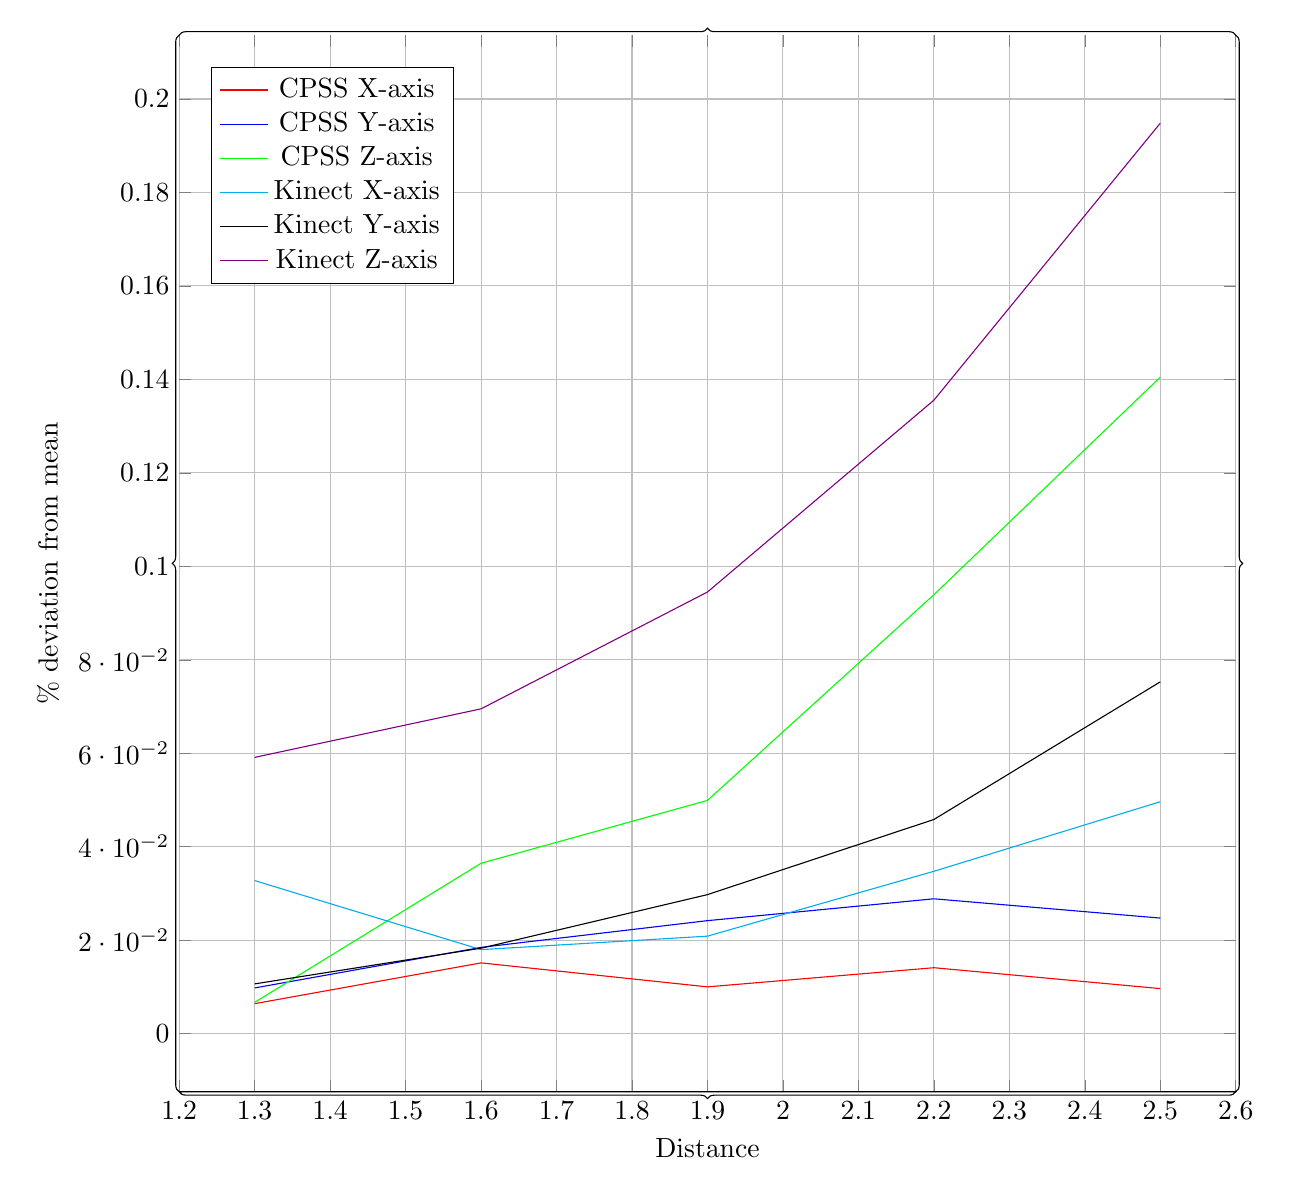
\begin{tikzpicture}
\begin{axis}[height=15cm,width=15cm,grid=major,xlabel=Distance,ylabel=\% deviation from mean,xmin=1.2,xmax=2.6,domain=1.2:2.6,legend entries={CPSS X-axis,CPSS Y-axis,CPSS Z-axis,Kinect X-axis,Kinect Y-axis,Kinect Z-axis},legend pos=north west]
%X-AXIS
\addplot [red] coordinates {(1.3,0.006418) (1.6,0.015143) (1.9,0.010009) (2.2,0.014109) (2.5,0.009640)}; %node [pos=0.1,pin={-10:$X$},inner sep=0pt] {};

%Y-AXIS
\addplot [blue] coordinates {(1.3,0.009779) (1.6,0.018461) (1.9,0.024181) (2.2,0.028856) (2.5,0.024728)}; %node [pos=0.3,pin={-10:$Y$},inner sep=0pt] {};

%Z-AXIS
\addplot [green] coordinates {(1.3,0.006695) (1.6,0.036458) (1.9,0.049911) (2.2,0.093916) (2.5,0.140487)}; %node [pos=0.6,pin={-10:$Z$},inner sep=0pt] {};


%Kinect data
%X-AXIS
\addplot [cyan] coordinates {(1.3,0.032756) (1.6,0.017977) (1.9,0.020863) (2.2,0.034741) (2.5,0.049633)}; %node [pos=0.2,pin={-10:$X$},inner sep=0pt] {};

%Y-AXIS
\addplot [black] coordinates {(1.3,0.010647) (1.6,0.018285) (1.9,0.029747) (2.2,0.045827) (2.5,0.075279)}; %node [pos=0.4,pin={-10:$Y$},inner sep=0pt] {};

%Z-AXIS
\addplot [violet] coordinates {(1.3,0.059115) (1.6,0.069500) (1.9,0.094501) (2.2,0.135550) (2.5,0.194821)}; %node [pos=0.7,pin={-10:$Z$},inner sep=0pt] {};


\end{axis}
\end{tikzpicture}
\caption{Distance versus precision along X,Y,Z axes}
\label{fig:dist_vs_prec}
\end{figure}
\noindent
Table 5-5 shows the dependence of measurement accuracy on distance for Kinect. Table 5-6 shows the dependence of measurement uncertainty on distance of measurement object from kinect sensor.

\begin{table}[ht]
\centering
\begin{tabular}{c c}
\hline\noalign{\smallskip}
Distance  & Kinect(\%  error) \\
\noalign{\smallskip}\hline\noalign{\smallskip}
1.3   & 1.194  \\
1.6   & 1.827  \\
1.9   & 1.911  \\
2.2   & 1.737  \\
2.5   & 1.057  \\
\noalign{\smallskip}\hline
\end{tabular}
\caption{Kinect:Dependence of measurement accuracy on distance}
\end{table}
\noindent

\begin{table}[ht]
\centering
\begin{tabular}{c c }
\hline\noalign{\smallskip}
Distance   & Kinect(\% uncertainty) \\
\noalign{\smallskip}\hline\noalign{\smallskip}
1.3    & 0.069 \\
1.6    & 0.191 \\
1.9    & 0.245 \\
2.2    & 0.261 \\
2.5    & 0.289 \\
\noalign{\smallskip}\hline
\end{tabular}
\caption{Kinect:Dependence of measurement uncertainty on distance}
\end{table}

\noindent
Although relative error in CPSS and Kinect doesn't gave a monotonous variation within the considered depth range but measurement uncertainty in kinect showed strict rise with increasing  distance from sensor. We can summarize these observations as average percentage relative error for CPSS was $\sim1.018\%$ while that for kinect was $\sim1.545\%$ within range of 1.3m-2.5m.Figure~\ref{fig:dist_vs_accuracy} represents the observed variation of measurement accuracy with distance, along with measurement uncertainty.

\begin{figure}[ht]
\centering
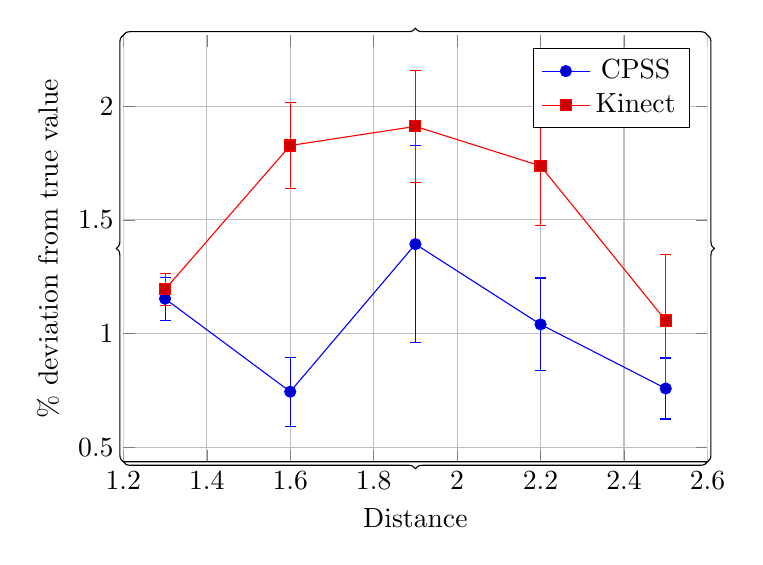
\begin{tikzpicture}
\begin{axis}[height=7cm,width=9cm,grid=major,xlabel=Distance,ylabel=\% deviation from true value,xmin=1.2,xmax=2.6,domain=1.2:2.6,legend entries={CPSS,Kinect},legend pos=north east]

\addplot +[blue,error bars/.cd,y dir=both,y explicit] coordinates {
(1.3,1.153) +- (0.0,0.095)
(1.6,0.744) +- (0.0,0.152) 
(1.9,1.393) +- (0.0,0.433)
(2.2,1.040) +- (0.0,0.204)
(2.5,0.758) +- (0.0,0.134)
};

\addplot +[red,error bars/.cd,y dir=both,y explicit] coordinates {
(1.3,1.194) +- (0.0,0.069)
(1.6,1.827) +- (0.0,0.191)
(1.9,1.911) +- (0.0,0.245)
(2.2,1.737) +- (0.0,0.261)
(2.5,1.057) +- (0.0,0.289)
};
\end{axis}
\end{tikzpicture}
\caption{Distance versus measurement accuracy with indication of uncertainty(vertical bars)}
\label{fig:dist_vs_accuracy}
\end{figure}






\subsection{Observations and conclusions}
\label{sec-4}
Kinect accuracy can be improved using system calibration[58][65][67][69].In our work we have used OpenNI default calibration parameters. Error-prone nature of both kinect and CPSS against surfaces with high reflectivity and very low reflectivity was observed. Further it was observed that due to disparity quantization multiple planes are visible in the scan of a single planar object and separation between these planes increases with increase in distance between object and sensor which was also reported by [63]. Here an approach is introduced for accuracy evaluation using 3D length measurements however deviations reported here may not be general statistics as [70] have observed different measurement accuracy for different units of kinect. Depth uncertainty in kinect is considerably higher than CPSS as shown in Tables 1 and 2. Although [71] reports relatively small improvement due to averaging over multiple measurements in range less than 3m, but it was found that the measurement uncertainty over 10 measurements was considerable(as shown in table 5.6) and should not be ignored, hence it suggests that averaging the measurements using multiple scans is important even within 2.5m.



\section{System calibration}
System calibration results in estimation of parameters which allow 3D sensor to map real-world 3D points defined in \textit{physical} units to 2D points defined in terms of \textit{pixels}. In this section, the tests performed to assess repeatability and accuracy of calibration algorithm are described. To assess repeatability, calibration was performed multiple times to determine \% average absolute deviation of estimated parameters from their mean values. For assessing accuracy, some \textit{reference} 3D points were selected whose 3D coordinates were known. These points were projected to camera/projector pixel coordinate space and the radial distance of projection from the \textit{observed} projection was considered as \textit{error}. A similar approach is described in [72]. The definition of \textit{system calibration error} $\varepsilon$ used in this work is described by the following equation:
\begin{equation}
\varepsilon=\frac{\sum_{i=1}^N\sqrt[2]{(X_t^i-X_e^i)^2+(Y_t^i-Y_e^i)^2}}{N}
\end{equation}
\noindent
$N$: Total 3D reference points used for testing system calibration parameters\newline
$(X_t^i,Y_t^i)$: True coordinates of 2D projection of $i^{th}$ reference point\newline
$(X_e^i,Y_e^i)$: 2D coordinates of $i^{th}$ reference point computed using system calibration parameters\newline

\subsection{Experiments and results}
Experiments to evaluate repeatability and accuracy of camera and projector intrinsic and extrinsic calibration parameters were performed. Procedure is already described in the parent section. For sake of brevity, equation 5.2 rephrases the relation used for projecting the $i^{th}$ reference point from real world 3D coordinates to 2D image coordinates in experiment for measuring accuracy of calibration parameters. Please refer section 2.1.2 for detailed explanation of this equation.
\begin{equation}
\begin{aligned}
& \begin{bmatrix}
U_e^i \\
V_e^i
\end{bmatrix} 
=A_c[R|T]\begin{bmatrix}
X_w^i \\
Y_w^i \\
Z_w^i
\end{bmatrix} \\
& \begin{bmatrix}
X_e^i \\
Y_e^i
\end{bmatrix}
=f(U_e^i,V_e^i)
\end{aligned}
\end{equation}
\noindent
where,\newline
$(X_w^i,Y_w^i,Z_w^i)$: 3D coordinates of $i^{th}$ reference point\newline
$(U_e^i,V_e^i)$: 2D undistorted coordinates of reference point in camera \newline
$A_c$: Camera intrinsic parameter matrix \newline
$[R|T]$: Camera extrinsic parameter matrix \newline
$f$: Camera distortion function estimated by calibration\newline
$(X_e^i,Y_e^i)$: 2D estimated coordinates of projection of reference point in camera image coordinate system\newline 
\noindent

\begin{enumerate}
\item{\textbf{Camera calibration}\newline}
In order to quantify the repeatability of the used OpenCV camera calibration algorithm which is an important measure of stability of any algorithm, we performed camera calibration 5 times and determined the \% average absolute deviation of its parameters. Table 5-7 shows the results.
\begin{table}[ht]
\centering
\begin{tabular}{c c}
\hline\noalign{\smallskip}
Parameter  & \% deviation \\
\noalign{\smallskip}\hline\noalign{\smallskip}
$f_x$   & 1.105  \\
$f_y$   & 1.075  \\
$c_x$   & 0.707  \\
$c_y$   & 0.894  \\
$k_1$   & 7.357 \\
$k_2$  &  8.825 \\
\noalign{\smallskip}\hline
\end{tabular}
\caption{Percentage average absolute deviation of camera calibration parameters}
\end{table}
\noindent
Results show considerably high uncertainty in estimating $k_1$ and $k_2$. This was observed for projector calibration as well(see table 5.9). So based on this test we can conclude that algorithm is repeatable within $\sim1\%$ for all parameters except distortion coefficients. Although more number of such tests can put more tighter and reliable limits.

Figure~\ref{fig:cam_calib_accuracy} shows the test scene with reference points which were used for estimating accuracy of calibration parameters. Coordinates of reference points were physically measured and used as \textit{true values}. Here true values were defined using corner-detection to detect image coordinates of reference points. Table 5-8 shows the result of projection of 3D points to camera image-space and their radial distance from corresponding \textit{observed} value. This test was repeatedly performed 5 times to reduce effect of random error in corner detection. 


\begin{figure}[ht]
\centering
\includegraphics[width=10cm,height=8cm]{../img_source/camera_calib_test.jpg}
\caption{Points A,B,C,D were used for measuring camera calibration accuracy}
\label{fig:cam_calib_accuracy}
\end{figure}






\begin{table}[ht]
\centering
\begin{tabular}{c c}
\hline\noalign{\smallskip}
Point  & Radial distance from true projection \\
\noalign{\smallskip}\hline\noalign{\smallskip}
A   & 2.553  \\
B   & 3.453  \\
C   & 4.080 \\
D   & 4.180 \\
\noalign{\smallskip}\hline
\end{tabular}
\caption{Camera calibration:Radial error of projection}
\end{table}
In table 5-8, radial error $\varepsilon$ points towards a systematic error since in all 5 measurements we observed that relation: $\varepsilon_{A}<\varepsilon_{B}<\varepsilon_{C}<\varepsilon_{D}$ holds, which demands further study.

\item{\textbf{Projector calibration}\newline}
During development it was observed that calibration parameters returned by OpenCV calibration algorithm for projector were not repeatable hence it was decided to use VPCLib[73] which gives considerably higher repeatability as shown in table 5-9.\newline
\indent
VPCLib assumes no distortion parameters in projector model. It estimates projector to 3D-plane homographies for multiple positions of projector with respect to plane. It further uses these homographies to compute points in 3D plane corresponding projector image points. Once these point correspondences are known it uses plane based calibration method for estimating the calibration parameters.  Further the estimated parameters are refined using \textit{Bundle adjustment} or non-linear minimization[73].\newline

\begin{table}[ht]
\centering
\begin{tabular}{c c c}
\hline\noalign{\smallskip}
Parameter  & OpenCV method & VPCLib method \\
\noalign{\smallskip}\hline\noalign{\smallskip}
$f_x$ & 7.625 & 2.166\\
$f_y$ & 7.445 & 2.047\\
$c_x$ & 5.559 & 1.795\\
$c_y$ & 4.381 & 1.861\\
$k_1$ & 38.196 & Not estimated\\
$k_2$ & 96.227 & Not estimated\\
\noalign{\smallskip}\hline
\end{tabular}
\caption{Percentage average absolute deviation of projector calibration parameters}
\end{table}
It can be clearly observed that VPCLib method gives much more repeatable results than OpenCV algorithm for projector calibration. Further it can observed that estimated $k_1$ and $k_2$ exhibit unacceptably high \% deviation. Hence VPCLib method was used for further analysis.\newline
\indent
As mentioned above, VPCLib method do not assume distortion parameters in projector model since projectors practically have negligible radial distortion hence $k_1$ and $k_2$ were not estimated and were assumed to be 0.\newline
To assess accuracy of projector intrinsic and extrinsic parameters estimated by VPCLib, 3D coordinates of corners of projection on a plane were determined through physical measurement and then they were reprojected back to projector image. Figure~\ref{fig:proj_calib_accuracy} shows the projected blank image whose corners were used for accuracy assessment. Radial distance between \textit{true} image coordinates and coordinates estimated through calibration parameters was considered as \textit{error}. Table 5-10 shows the deviation between observed and estimated 2D projector coordinates. Here again we observe a pattern in radial error in which error is monotonically increasing from point A to point D which is similar to that was observed in case of camera calibration in table 5-8.
\begin{figure}
\centering
\includegraphics[width=10cm,height=8cm]{../img_source/proj_calib_test.jpg}
\caption{Corners A,B,C,D were used for assessing accuracy of projector calibration parameters}
\label{fig:proj_calib_accuracy}
\end{figure}

\begin{table}[ht]
\centering
\begin{tabular}{c c}
\hline\noalign{\smallskip}
Point  & Radial distance from true projection \\
\noalign{\smallskip}\hline\noalign{\smallskip}
A   &  6.776 \\
B   &  8.608 \\
C   &  11.728\\
D   &  18.248\\
\noalign{\smallskip}\hline
\end{tabular}
\caption{Projector calibration:Radial error of projection}
\end{table}
\end{enumerate}

\subsection{Limitations of the used testing method}
This approach requires us to define \textit{true} 3D reference coordinates which is not practical at larger distances from reference origin without using a CMM machine or any other highly accurate metrology equipment. Hence this approach do not allow to practically cover entire \textit{calibration volume} to define accuracy of calibration parameters in general. Hence there is a need of an \textit{automated} method which can efficiently cover entire calibration volume without any requirement of manual intervention to define true values for 3D reference points. Even for exhaustive testing at distance where true 3D coordinates can be conveniently measured it is very time consuming process. Further to define $(X_t^i,Y_t^i)$ we need to use a \textit{feature detector} which in itself will add corner detection errors.  



\section{Stereo correspondence}
Stereo-correspondence relates pixels in camera and projector image which corresponds to a common point in real world. To assess accuracy of stereo-correspondence achieved using coded phase shift technique a \textit{known} checkerboard pattern was projected. Corners of checkerboard were detected and corresponding projector coordinates were determined using the stereo-correspondence estimated using coded phase shift technique. Accuracy is defined to be the \textit{radial} distance of estimated projector coordinates for detected checkerboard corners from the true coordinates of the checkerboard corners in projector image. The definition of \textit{stereo-correspondence error} used in this work is described by the following equation:
\begin{equation}
\varepsilon=\frac{\sum_{i=1}^N\sqrt[2]{(X_t^i-X_e^i)^2+(Y_t^i-Y_e^i)^2}}{N}
\end{equation}
\noindent
where,\newline
$N$: Total number of checkerboard corners used for testing stereo-correspondence \newline
$(X_t^i,Y_t^i)$: True coordinates of $i^{th}$ checkerboard corner\newline
$(X_e^i,Y_e^i)$: Estimated coordinates of $i^{th}$ checkerboard corner

\subsection{Experiments and results} 
Stereo-correspondence for a phase-shift technique is mainly affected by non-linear output response of projection and capture devices to the applied input[7][42]. This non-linearity can be compensated by a factor called \textit{gamma}. Projector Gamma allows manipulation of contrast of projected image such that non-linearity of input-to-output behavior of projector can be compensated. Furthermore a projected sinusoidal pattern can \textit{appear} non-sinusoidal if contrast of projected image has not been controlled to suppress non-linearity of device. Although same holds for camera also but in this work we have limited our scope to study the effects of projector gamma.\newline
\indent
Incorrect value of gamma leads to apparent \textit{waviness} in the 3D reconstructions as shown in figure~\ref{fig:gamma_3_phase} which shows the zoomed view of reconstruction of a planar object for different values of gamma. Here $\gamma=2.041$ seems to be more accurate gamma value since planarity of reconstructed surface is higher than that for $\gamma=1.0$.
\begin{figure}[htbp]
\def\tabularxcolumn#1{m{#1}}
\begin{tabularx}{\linewidth}{@{}cXX@{}}
\begin{tabular}{c c}
\subfloat[$\gamma=1.0$]{\includegraphics[width=7cm,height=7cm]{../img_source/3_phase_1_test_2.jpg}} & 
\subfloat[$\gamma=2.041$]{\includegraphics[width=7cm,height=7cm]{../img_source/3_phase_2_041_test_2.jpg}}\\
\end{tabular}
\end{tabularx}
\caption{Effect of gamma on 3D reconstruction of a plane}
\label{fig:gamma_3_phase}
\end{figure}
Clearly this will affect the measurement accuracy of the system. So the target in this work was to study the effect of projector gamma on stereo-correspondence error.\newline
\indent Further, in literature it has been reported that effect of non-linearity reduces with increasing number of phase shifted patterns used to acquire stereo-correspondence[7]. This can be observed in figure~\ref{fig:gamma_3_4_5} which shows reduction in \textit{waviness} in zoomed view of reconstruction of a planar object using 4 and 5 phase shifted patterns as compared to 3 phase shifted patterns. Hence,it was further attempted to quantify the effect of number of phase shifted patterns on stereo-correspondence error.
\begin{figure}[ht]
\def\tabularxcolumn#1{m{#1}}
\begin{tabularx}{\linewidth}{@{}cXX@{}}
\begin{tabular}{c c}
\subfloat[3 phase]{\includegraphics[width=7cm,height=7cm]{../img_source/phase_3_edit.jpg}} &
\subfloat[4 phase]{\includegraphics[width=7cm,height=7cm]{../img_source/phase_4_edit.jpg}}\\
\subfloat[5 phase]{\includegraphics[width=7cm,height=7cm]{../img_source/phase_5_edit.jpg}} \\
\end{tabular}
\end{tabularx}
\caption{Effect of increasing number of phase shifted patterns on \textit{waviness} in 3D reconstruction}
\label{fig:gamma_3_4_5}
\end{figure}
\FloatBarrier
\noindent Tests as already described in the parent section were performed for both cases i.e., varying gamma for 3 phase shifted pattern approach and by varying the number of projected phase-shifted fringe patterns under a constant gamma($\gamma=1$). Table 5.11 shows the effect of projector gamma on stereo-correspondence error. Table 5.12 shows the effect of increasing number of phase-shifted patterns on stereo-correspondence error.   

\begin{table}[htbp]
\centering
\begin{tabular}{c c}
\hline\noalign{\smallskip}
Gamma($\gamma$)  & Stereo-correspondence error \\
\noalign{\smallskip}\hline\noalign{\smallskip}
1.0   &  1.890\\
1.524   &  1.682 \\
1.912   &  1.730\\
2.041   &  1.588\\
2.559 & 2.073\\
2.947 & 2.394\\
\noalign{\smallskip}\hline
\end{tabular}
\caption{Stereo-correspondence error for various gamma values for 3 phase-shifted method}
\end{table}

\begin{table}[htbp]
\centering
\begin{tabular}{c c}
\hline\noalign{\smallskip}
Number of patterns  & Stereo-correspondence error \\
\noalign{\smallskip}\hline\noalign{\smallskip}
3   &  1.890 \\
4   &  2.100 \\
5   &  2.454\\
\noalign{\smallskip}\hline
\end{tabular}
\caption{Stereo correspondence error for 3,4,5 phase shifted patterns}
\end{table}
\noindent


In table 5.11 it can be observed that there is reduction in stereo-correspondence error from $\gamma=1.0$ to $\gamma=2.041$ followed by increase monotonous increase in error from $\gamma=2.559$. But in table 5.12 we got contradictory results to our expectation. To further confirm this observation we performed experiment 5 times but same pattern of monotonous increase in correspondence error from 3 to 5 phase shifted patterns was observed. This highlights the shortcomings of used criteria for stereo-correspondence error. Although criteria is correct in its formulation because if increasing number of phase-shifted patterns reduces effect of system non-linearity as has been observed in figure~\ref{fig:gamma_3_4_5} then it must result in reduction in stereo-correspondence error as defined here. It encourages for further study on how to apply this criteria correctly. 

\subsection{Limitations of the used testing method}
This approach works as long as projected features can be uniquely recognized so that explicit correspondence estimation for the reference pattern features itself is not required. This can be conveniently used for assessing stereo-correspondence errors in case of a planar scene with no occlusions, since correspondence between camera and projector for feature points in the reference pattern can be easily established. But for complex surfaces with surface discontinuities, curvature, where correspondence between camera and projector for reference pattern cannot be implicitly assumed we either have to use any other technique to define correspondence for the features or an altogether different approach to test stereo-correspondence. Further, accuracy of feature detection will also affect the computed correspondence error.


\section{Triangulation}
Triangulation as described in chapter-4 computes 3D coordinates of a real-world point given stereo-correspondence between camera-projector and system calibration parameters. Although it is already mentioned that accuracy evaluation of optical triangulation cannot be done reliably unless we have exact quantitative error bounds for calibration and correspondence for any test case, it is possible to compare different triangulation methods with respect to the accuracy of estimated 3D coordinates of any feature in the scene without changing correspondence and system calibration parameters in the process. This approach do not require us to have knowledge about \textit{exact} error bounds of correspondence and calibration. Hence it is proposed to define \textit{triangulation error} as the deviation of estimated 3D coordinates of a feature in the scene with respect to that reported by CMM machine. Here coordinate measurement is proposed rather than conventional dimension measurement since coordinate measurement indirectly reflects accuracy of dimensions.








\section{Summary}
In this chapter, the approaches used for assessing accuracy of stereo-correspondence and system calibration parameters was described along with the limitations of such approaches. Furthermore, a test was proposed to evaluate accuracy of optical triangulation which was not in the scope of work due to time limitations.\newline
\indent In addition, comparison of measurement accuracy and precision of developed system with Microsoft Kinect has been described. Here we examined reconstruction accuracy in static scenes and observed that within depth range of 1.3m-2.5m(based on combine depth-of-field of camera projector system) kinect reconstructs with ~0.5 percent higher relative error as compared to CPSS, further the precision of 3D data generated by both techniques using reconstruction of a planar object at various distances was analyzed, and it was observed that for both kinect and CPSS, there is a strong relationship between distance of object from sensor and uncertainty in measurement. Overall CPSS exhibits relatively lower uncertainty in X,Y,Z, coordinates. Furthermore it was observed that CPSS has almost equal uncertainties in X,Y,Z coordinates but kinect exhibits considerably higher uncertainty along Z-axis(depth-uncertainty) as compared to that along X and Y axes.

 

\chapter{Conclusions and future works}
In this chapter, conclusions from the work performed, original contributions of this work and possible future directions emerging from this work will be discussed. Section 6-1 describes the conclusions and propose future directions from the work done on system calibration and stereo-correspondence. Section 6-2 describes the original contributions of this work.

\section{Conclusions and proposed future works}
\begin{enumerate}
\item \textbf{System calibration} \newline
Development and accuracy evaluation of system calibration module offered following insights: 
\begin{enumerate}
\item As mentioned in table 5.7 repeatability of camera calibration parameters using OpenCV method was within $\sim1\%$
except distortion coefficients. While this may be sufficiently reliable for some applications but for domains like dental transplantations, CFD, inspection of fabricated job where very high accuracy and repeatability of metrology device is expected this range of repeatability may not be sufficient. Recently [11] have proposed an algorithm which they claim to provide appreciably higher accuracy than commonly used OpenCV method. Hence our future work includes experimenting with this algorithm to evaluate its accuracy to assess its applicability in the domains mentioned above. 

\item Furthermore, higher values of \% deviation for $k_1$ and $k_2$ possibly suggest instability of the calibration algorithm in estimating $k_1$ and $k_2$. In this work high quality lenses were used, hence it may be due to \textit{overfitting} leading to estimating coefficients for radial distortion even though lens may not have significant distortion.   

\item For projector calibration table-5.9 clearly showed that OpenCV based calibration method cannot be reliably used due to unacceptably high values of \% deviations for estimated parameters. Instead a study should be done to determine the reason why this algorithm do not reliably works for projector although it works for camera calibration. This question is significant because projector is modeled as \textit{inverse camera}.

\item To make the developed system more flexible and mobile, there is need to account for world coordinate system internally or by precalibrating system for physical units like as done in kinect. This will remove the constraint on the system to position world coordinate system within measurement volume which can be inconvenient and cumbersome at times.  

\item During calibration, subpixel corner detection algorithm was used. It needs multiple initial parameters decision of which considerably changes the position of the detected corner and hence the estimated calibration parameters. But in our knowledge, there has been no thorough study of optimal parameters for certain level of desired accuracy of subpixel corner coordinates or a study relating optimal choice of parameters with structure of image.
\end{enumerate}


  

\item \textbf{Stereo-correspondence} \newline
Work on stereo-correspondence provided practical insight into coded phase-shift technique:
\begin{enumerate}
\item In practice it was observed that coded phase shift technique is ineffective in highly specular or reflective environments. Furthermore it is not suitable to be used outdoors. It is primarily because the currently used illumination model for phase shift technique does not take such factors into account.

\item Pattern acquisition time is the main hurdle in allowing one to do real-time 3D scanning using this technique. Therefore, there is need to reduce number of projected pattern. This will be part of our future work.

\item It was observed that non-sinusoidal nature of captured patterns depends upon camera gamma, environmental lighting, camera resolution, perspective of camera with respect to region in the scene where pattern is projected etc., in addition to projector gamma. Hence there is a need of a study to account for all these factors besides projector gamma.

\item Further a problem of locating edge of projected binary coded patterns in camera image was encountered. Strip edge region is ambiguous for decoding binary codewords since it typically has grey intensity hence it cannot be classified as black or white only. In this work, pixels corresponding to such regions were discarded and were considered as invalid. This has raised the need for an algorithm which can atleast approximately determine the position of strip edge.  

\item It was initially attempted to develop system solely based on phase-shift method without any supporting technique like binary coded patterns but unacceptably poor time efficiency of the algorithm used for phase-unwrapping was observed hence it was decided to changed it to combination of binary coded and phase shift methods. It reduces computational complexity of phase-unwrapping but increases pattern acquisition time. To reduce this time and problems of strip edge detection with binary coded patterns, it is proposed to develop a time efficient phase unwrapping algorithm which will allow us to solve stereo-correspondence using only phase-shift approach. This will considerably reduce the required number of patterns. 

\item During experiments with stereo-calibration module it was observed that the proposed \textit{stereo-correspondence error} criterion gives different error estimates under different lighting conditions. Hence it has been proposed to study the effect of various radiometric conditions on the behavior of this criterion. And it is further speculated that contradictory results obtained in table 5.12 require accommodation of radiometric conditions into account. 
\end{enumerate}



\vspace{1cm}
\item \textbf{3D reconstruction and triangulation}\newline
It is possible to improve the time efficiency of system by replacing ray-ray triangulation which requires projection of both horizontal and vertical patterns as described in chapter-3 to ray-plane triangulation which calculates 3D coordinates of a point using intersection of an optical ray from camera and corresponding plane from projector or vice versa. Ray-plane triangulation will require projection of only vertical or horizontal patterns thereby reducing the required number of patterns by half. \newline
Furthermore, for our application of dental imaging, CFD and inspection of fabricated jobs it is required to have complete 3 dimensional view of the object. For this purpose it is proposed to extend the developed system such that it allows user to take complete 360 degree view of the object.   

\end{enumerate}


\section{Contributions of this work}
This work is focused on development and accuracy analysis of a 3D scanner, where in both development and accuracy evaluation some novelties are observed:
\begin{enumerate}
\item Developed system is first \textit{in-house} 3D measurement system based on Coded phase-shift technique which is currently among the most accurate 3D metrology approaches based on active vision.

\item The measurement accuracy and precision of developed system  was experimentally studied and compared with Microsoft Kinect, this work can be of immediate use to researchers and practitioners planning to use kinect for accuracy and reliability critical tasks. 

\item An approach to assess \textit{measurement accuracy} was proposed and experimentally demonstrated.  

\item A \textit{Stereo-correspondence error} criteria has been proposed and experimentally demonstrated which will allow us to evaluate accuracy of stereo-correspondence.   
\end{enumerate}


%% This defines the bibliography file (main.bib) and the bibliography style.
%% If you want to create a bibliography file by hand, change the contents of
%% this file to a `thebibliography' environment.  For more information 
%% see section 4.3 of the LaTeX manual.
\begin{singlespace}
\begin{thebibliography}{10000000000}
\bibitem{1} %1
Microsoft Photosynth.\newline 
photosynth.net\newline
Accessed 3 December 2012

\bibitem{2} %2
Projective geometry tutorial.\newline 
http://www.cse.iitd.ernet.in/~suban/vision/tutorial/node1.html \newline
Accessed 4 December 2012

\bibitem{3} %3
Faugeras,Olivier.(1995).Stratification of 3-D vision: projective, affine, and metric representations,Journal of the Optical Society of America A,Vol-12,46548--4 


\bibitem{4} %4
Hartley,Richard I.,Sturm,Peter(1997).Triangulation, 
Computer Vision and Image Understanding,Volume 68, Issue 2, November 1997,Pages 146-157 

\bibitem{5}  %5
Saxena,Ashutosh,Sun,Min,Ng,Andrew Y.(2007).3-D Reconstruction from Sparse Views using Monocular Vision,ICCV workshop on Virtual Representations and Modeling of Large-scale environments (VRML),2007  

\bibitem{6} %#
Flexiscan3D scanner software \newline
http://www.3d3solutions.com/products/flexscan3d/ \newline
Accessed:3 December 2012

\bibitem{7} %#
Pan,B., Kemao,Q.,Huang,L.,and Asundi,A.(2009).Phase error analysis and compensation for nonsinusoidal waveforms in phase-shifting digital fringe projection profilometry, Opt. Lett.  34, 416-418. 

\bibitem{8} %#
Tsai,Roger Y. (1987) :A Versatile Camera Calibration Technique for High- 
Accuracy 3D Machine Vision Metrology Using Off-the-Shelf TV Cameras 
and Lenses,IEEE Journal of Robotics and Automation, Vol. RA-3, No. 4, 
August 1987, pp. 323-344. 

\bibitem{9} %#
Zhang,Song(2005).High-resolution, Real-time 3-D Shape Measurement,Ph.D. dissertation, Stony Brook University, Stony Brook, NY, 2005. 

\bibitem{10} %#
Zhang,Z.(2000).A flexible new technique for camera calibration. IEEE Transactions on Pattern Analysis and Machine Intelligence, 22(11):1330-1334, 2000 

\bibitem{11} %#
Vo,Minh,Wang,Zhaoyang,Pan,Bing,Pan,Tongyan(2012).Hyper-accurate flexible calibration technique for fringe-projection-based three-dimensional imaging,Opt. Express 20, 16926-16941 (2012) 

\bibitem{12} %#
Hartley,R.I.(1994),An algorithm for self calibration from several viewes.In Proceedings of IEEE Conference on Computer Vision and Pattern Recognition,pages 908-912,IEEE Computer Society Press 

\bibitem{13} %#
Luong,Q.~T,Faugeras,O.(1997).Self-calibration of a moving camera from point correspondences and fundamental matrices.The International Journal of Computer Vision,22(3):261-289,1997 

\bibitem{14} %#
Caprile,B,Torre,V.(1990).Using Vanishing Points for Camera Calibration.The International Journal Of Computer Vision,4(2):127-140,Mar.1990 

\bibitem{15} %#
Hartley,R.(1994).Self-calibration from multiple views with a rotating camera.In Proceedings of 3rd ECCV,volume 800-801 of 'Lecture notes in Computer Science' pages 471-478,Stockholm,Sweden,May 1994.Springer-Verlag 

\bibitem{16} %#
Zollner, Helmut and Sablatnig,Robert(2004).Comparison of Methods for Geometric Camera Calibration using Planar Calibration Targets,Proceedings of the 28th Workshop of the Austrian Association of Pattern Recognition, AAPR 2004,pp.237--244,OCG Schriftenreihe, {\"O}sterreichische Arbeitsgemeinschaft f{\"u}r Mustererkennung

\bibitem{17} %#
Heikkil\"{a},J.,Silven,O.(1997).A Four-Step Camera Calibration Procedure with Implicit Image Correction.
In Proc. of IEEE Computer Vision and Pattern Recognition, pp. 1106-1112, 1997

\bibitem{18} %#
Camera Calibration Toolbox For Matlab \newline
http://www.vision.caltech.edu/bouguetj/calib\_doc/index.html \newline
Accessed:3 December 2012 

\bibitem{19} %#
OpenCV documentation on Camera calibration \newline
http://docs.opencv.org/modules/calib3d/doc/calib3d.html \newline
Accessed 5 December 2012

\bibitem{20} %#
Levenberg Marquardt algorithm.\newline
http://en.wikipedia.org/wiki/Levenberg\%E2\%80\%93Marquardt\_algorithm \newline
Accessed 4 December 2012.

\bibitem{21} %# 
Extrinsic parameters estimation in OpenCV\newline 
http://opencv.willowgarage.com/documentation/camera\_calibration\_and\_3d\newline
\_reconstruction.html\#findextrinsiccameraparams2 \newline
Accessed 5 December 2012

\bibitem{22} %#
Bradski,Gary and Kaehler,Adrian(2008).Learning OpenCV,Computer Vision with the OpenCV Library.O'Reilly Media,September 2008 

\bibitem{23} %#
Asla Medeiros e Sa,Esdras Soares de Medeiros Filho,Paulo Cezar Carvalho,Luiz Velho.Coded Structured Light for 3D-photography:an Overview.\newline
www.visgraf.impa.br/Data/RefBib/PS\_PDF/rita-survey/survey.pdf \newline
Accessed 5 December 2012
  

\bibitem{24} %#
Salvi,J.,Pag\`es,J,Tutorial on Coded Light Projection techniques\newline 
http://eia.udg.es/~qsalvi/Tutorial\_Coded\_Light\_Projection\_Techniques\_arc\newline
hivos/v3\_document.html \newline
Accessed 4 December 2012

\bibitem{25} %#
Geng,J.(2011)."Structured-light 3D surface imaging: a tutorial," Adv. Opt. Photon.3, 128-160 .

\bibitem{26} %#
Pag\`es,Jordi,Salvi,Joaquim,Garcia,Rafael,Matabosch,Carles(2003).Overview of coded light projection techniques for automatic 3D profiling 

\bibitem{27} %#
Posdamer,J. L.,Altschuler,M. D.(1982). Surface measurement by 
space-encoded projected beam systems, Comput. Graph. Image Processing 
18(1), 1-17 (1982). 

\bibitem{28} %#
Inokuchi,S.,Sato,K.,Matsuda,F.(1984).Range-imaging for 3-D object recognition, 
in International Conference on Pattern Recognition (International 
Association for Pattern Recognition, 1984), pp. 806-808. 

\bibitem{29} %#
Caspi,D.,Kiryati,N.,Shamir,J.(1998),Range imaging with adaptive color 
structured light, IEEE Trans. Pattern Anal. Mach. Intell. 20(5), 470-480 
(May 1998). 

\bibitem{30} %#
Horn,Eli,Kiryati,Nahum(1997).Toward Optimal Structured Light Patterns,Image and Vision Computing,Vol. 17,pp.87-97 

\bibitem{31} %#
Ghiglia,Dennis C.,Pritt,Mark D..Two-Dimensional Phase Unwrapping: Theory, Algorithms, and Software.Wiley Publications,ISBN: 978-0-471-24935-1

\bibitem{32} %#
MacWilliams,F.J.,Sloane,N.J.A.(1976).Pseudorandom sequences and 
arrays, Proc. IEEE 64(12), 1715-1729. 

\bibitem{33} %#
De Bruijn sequnces\newline 
http://feed-back.be/nick/?page\_id=310\newline
Accessed 12 December 2012

\bibitem{34} %#
Moigne,J.Le,Waxman,A. M.(1985), Multi-resolution grid patterns for 
building range maps,in Vision-85, Applied Machine Vision Conference 
(ASME) (Society of Manufacturing Engineers, 1985), pp. 22-39. 

\bibitem{35} %#
Ulusoy,A. Osman,Calakli,F.,Taubin,G.(2009), One-shot scanning using De 
Bruijn spaced grids, in 2009 IEEE 12th International Conference on Computer 
Vision Workshops (ICCV Workshops) (IEEE, 2009), pp. 1786-1792. 
 
\bibitem{36} %#
Carrihill,B.,Hummel,R.(1985). Experiments with the intensity ratio depth sensor. In Computer Vision, Graphics and Image 
Processing, volume 32, pages 337--358. Academic Press, 1985 

\bibitem{37} %#
Chazan,G.,Kiryati,N.(1995). Pyramidal intensity ­ratio depth sensor. Technical report 121, Center for Communication and Informa­tion Technologies, Department of Electrical Engineering, Technion, Haifa, Israel, October 1995. 

\bibitem{38} %#
Hung,D.C.D.(1993). 3d scene modelling by sinusoid encoded illumination. Image and Vision Computing, 11:251--256, 1993. 

\bibitem{39} %#
Tajima,J.,Iwakawa,M.(1990). 3D data acquisition by rainbow range finder. In International Conference on Pattern Recognition, pages 309--313, 1990 

\bibitem{40} %#
Sato,T.(1999). Multispectral pattern projection range finder. In Proceedings of the Conference on ThreeDimensional Image Capture and Applications II, volume 3640, pages 28--37, San Jose, California, January 1999. SPIE. 

\bibitem{41} %#
Stripe boundary codes for real-time structured-light range scanning of moving 
objects. In The 8th IEEE International Conference on 
Computer Vision, pages II: 359-366, 2001. 

\bibitem{42} %#
Zhang,Song(2010).Recent progresses on real-time 3D shape measurement using digital fringe projection techniques.Optics and Lasers in Engineering, Volume 48, Issue 2, February 2010, Pages 149-158 

\bibitem{43} %#
Gorthi,S.S.,Rastogi,P(2009).Fringe projection technique:Whither we are?.Optics and Lasers in Engineering, 2009 

\bibitem{44} %#
`open-light'-Google code \newline
http://code.google.com/p/open-light/\newline
Accessed 5 December 2012 

\bibitem{45} %#
`Structured-light'-Goole code \newline
http://code.google.com/p/structured-light/ \newline
Accessed 5 December 2012

\bibitem{46} %#
Gupta,Mohit and Agrawal, Amit and Veeraraghavan, Ashok and Narasimhan, Srinivasa,G.(2012).A Practical Approach to 3D Scanning in the Presence of Interreflections,Subsurface Scattering and Defocus.International Journal of Computer Vision,pp.1-23,Springer

\bibitem{47} %#
Ghiglia,Dennis C.,Romero,Louis A.(1996)."Minimum Lp-norm two-dimensional phase unwrapping," J. Opt. Soc. Am. A 13, 1999-2013 (1996)

\bibitem{48} %#
Mundy,J.,Zisserman,A.(1992).Appendix:Projective geometry for machine vision-Geometric invariances in computer vision,MIT Press,1992 
 

\bibitem{49} %#
R.I.,Hartley,Zisserman,A.(2004).Multiple View Geometry in Computer Vision,Second edition,Cambridge University Press, ISBN:0521540518
  
\bibitem{50} %#
Hartley,R.,Gupta,R.,Chang,T.(1992).Stereo from uncalibrated cameras, 
in Proceedings, IEEE Conference on Computer Vision and Pattern Recognition, 1992, pp. 761-764. 

\bibitem{51} %#
Triangulation\newline 
http://en.wikipedia.org/wiki/Triangulation\newline
Accessed 5 December 2012

\bibitem{52} %#   
Brett R.,Jones(2010).AUGMENTING COMPLEX SURFACES WITH PROJECTOR-CAMERA SYSTEMS,M.S.Thesis,University of Illinois at Urbana-Champaign

\bibitem{53} %#
Point cloud library.\newline
pointclouds.org/.\newline
Accessed 24 November 2012

\bibitem{54} %#
Accuracy \& precision.\newline
http://en.wikipedia.org/wiki/Accuracy\_and\_precision\newline
Accessed 24 November 2012

\bibitem{55} %#
OpenCV function for checkerboard corner detection.\newline
http://opencv.willowgarage.com/documentation/camera\_calibration\_and\_3d\_\newline
reconstruction.html\#findchessboardcorners\newline
Accessed 24 November 2012

\bibitem{56} %#
Sansoni,G., Carocci,M., and Rodella,R.(1999). "Three-Dimensional Vision Based on a Combination of Gray-Code and Phase-Shift Light Projection: Analysis and Compensation of the Systematic Errors," Appl. Opt.  38, 6565-6573 .

\bibitem{57} %#
Microsoft Kinect.\newline
http://www.xbox.com/en-US/KINECT.\newline
Accessed 24 November 2012

\bibitem{58} %#
OpenNi home page.\newline
openni.org/.Accessed 24 November 2012

\bibitem{59} %#
OpenKinect home page.\newline
openkinect.org/.Accessed 24 November 2012

\bibitem{60} %#
RGBDemo program for accessing kinect data.\newline
labs.manctl.com/rgbdemo/ \newline
Accessed 24 November 2012

\bibitem{61} %#
Skanect for Windows \& Mac-plateform.\newline
http://manctl.com/products.html.\newline
Accessed 24 November 2012

\bibitem{62} %#
Code laboratory.\newline
http://codelaboratories.com/nui/.\newline 
Accessed 24 November 2012

\bibitem{63} %#
Khoshelham, K., Elberink, S.O.(2012). Accuracy and Resolution of Kinect Depth Data for Indoor Mapping Applications. Sensors, 12, 1437-1454.

\bibitem{64} %#
Freedman, B., Shpunt, A., Machline, M., \& Arieli, Y. (2010).
Patent No. US2010/0018123 A1. United States of America.

\bibitem{65} %#
Smisek, J., Jancosek, M., Pajdla, T., (2011), "3D with Kinect," Computer Vision Workshops (ICCV Workshops),pp.1154-1160, 6-13 Nov. 2011
doi: 10.1109/ICCVW.2011.6130380

\bibitem{66} %#
ifixit Kinect teardown.\newline
http://www.ifixit.com/Teardown/Microsoft+Kinect+Teardown/4066/1.\newline
Accessed 24 November 2012

\bibitem{67} %#
ROS kinect calibration page. \newline
http://www.ros.org/wiki/openni\_launch/Tutorials/IntrinsicCalibration?actio\newline
n=show\&redirect=openni\_camera\%2Fcalibration.\newline
Accessed 24 November 2012

\bibitem{68} %#
Moln\`ar,B., Toth,C.K., and Detrek\"{o}i,A.(2012). ACCURACY TEST OF MICROSOFT KINECT FOR HUMAN MORPHOLOGIC MEASUREMENTS, Int. Arch. Photogramm. Remote Sens. Spatial Inf. Sci., XXXIX-B3, 543-547, doi:10.5194/isprsarchives-XXXIX-B3-543-2012

\bibitem{69} %#
Herrera C.,D.,Kannala, J.,Heikkil\"{a},J.(2012).Joint depth and color camera calibration with distortion correction, TPAMI,.

\bibitem{70} %#
Boehm,J.(2012).NATURAL USER INTERFACE SENSORS FOR HUMAN BODY MEASUREMENT, Int. Arch. Photogramm. Remote Sens. Spatial Inf. Sci., XXXIX-B3, 531-536, doi:10.5194/isprsarchives-XXXIX-B3-531-2012

\bibitem{71} %#
Chow,J.C.K.,Ang,K.D.,Lichti,D.D.,and Teskey,W.F.(2012). 
PERFORMANCE ANALYSIS OF A LOW-COST TRIANGULATION-BASED 3D
CAMERA: MICROSOFT KINECT SYSTEM
International Archives of the Photogrammetry, Remote Sensing and Spatial Information Sciences, Volume XXXIX-B5
XXII ISPRS Congress

\bibitem{72} %#
Salvi,Joaquim,Armangu\`e,Xavier,Batlle,Joan(2002).A comparative review of camera calibrating methods with accuracy evaluation, Pattern Recognition, Volume 35, Issue 7, July 2002, Pages 1617-1635, ISSN 0031-3203, 10.1016/S0031-3203(01)00126-1.

\bibitem{73} %#
Drar\`eni, J. and  Roy, S. and Sturm, P.(2012).Methods for Geometrical Video Projector Calibration,Machine Vision and Applications

\end{thebibliography}
\end{singlespace}


\end{document}

